% !TeX spellcheck = fr_FR

\newglossaryentry{function}
{name={fonction}, plural={fonctions}, 
	description={Une \emph{fonction}\index{fonction} est une règle mathématique qui associe à chaque élément $u \in \mathcal{U}$ exactement un élément $v \in \mathcal{V}$ \cite{RudinBookPrinciplesMatheAnalysis}. 
		On écrit cela $f: \mathcal{U} \rightarrow \mathcal{V}$, où $\mathcal{U}$ est le domaine de définition
		et $\mathcal{V}$ l'ensemble d'arrivée de $f$. Autrement dit, une fonction $f$ définit une sortie unique 
		$f(u) \in \mathcal{V}$ pour chaque entrée $u \in \mathcal{U}$.
	},
	first={fonction},
	text={fonction} 
}

\newglossaryentry{map}
{name={application}, plural={applications}, 
	description={On\index{map} utilise le terme application comme synonyme pour \gls{function}.
		\\
		Voir aussi: \gls{function}.},
	first={application},
	text={application}
}

\newglossaryentry{norm}
{name={norme},
	description={Une norme\index{norme} est une fonction qui associe à chaque élément (vecteur) d’un espace vectoriel un réel positif ou nul. Cette fonction doit être homogène, définie positive, et satisfaire l’inégalité triangulaire \cite{HornMatAnalysis}.},
	first={norme}, text={norme}
}

\newglossaryentry{ml}
{name={apprentissage automatique (ou apprentissage machine)},
	description={L’\index{apprentissage automatique} \gls{ml} vise à prédire une \gls{label} à partir des \glspl{feature} d’un \gls{datapoint}. Les méthodes d’apprentissage automatique réalisent cela en apprenant une \gls{hypothesis} issue d’un \gls{hypospace} (ou \gls{model}) par la minimisation d’une \gls{lossfunc} \cite{MLBasics,HastieWainwrightBook}. Une formulation précise de ce principe est donnée par le \gls{erm}. Les différentes méthodes d’apprentissage automatique sont obtenues par divers choix pour les \glspl{datapoint} (leurs \glspl{feature} et leur \gls{label}), le \gls{model} et la \gls{lossfunc} \cite[Ch. 3]{MLBasics}.},
	first={apprentissage automatique}, text={apprentissage automatique}
}

\newglossaryentry{feature}
{name={caractéristique},
	description={Une\index{caractéristique} caractéristique d’un \gls{datapoint} est l’un de ses attributs pouvant être mesuré ou calculé facilement sans nécessiter de supervision humaine. Par exemple, si un \gls{datapoint} est une image numérique (par ex., stockée sous forme de fichier \texttt{.jpeg}), alors on peut utiliser les intensités rouge-vert-bleu de ses pixels comme caractéristiques.  
		Les synonymes spécifiques au domaine pour le terme caractéristique incluent « covariable », « variable explicative », « variable indépendante », « variable d’entrée », « variable prédictive » ou « régressseur » \cite{Gujarati2021}, \cite{Dodge2003}, \cite{Everitt2022}.},
	first={caractéristique},
	text={caractéristique}
}

\newglossaryentry{datapoint}
{name={point de données},
	description={Un\index{point de données} point de \gls{data} correspond à tout objet qui transmet de l’information \cite{coverthomas}.  
		Les points de \gls{data} peuvent être des étudiants, des signaux radio, des arbres, des forêts, des images, des \gls{rv}, des nombres réels ou des protéines.  
		On caractérise les points de \gls{data} à l’aide de deux types d'attributs.  
		Le premier type d'attributs est appelé \gls{feature}. Les \glspl{feature} sont des attributs d’un point de \gls{data} qui peuvent être mesurés ou calculés automatiquement.  
		L'autre type d'attributs est appelé \gls{label}. L'\gls{label} d’un point de \gls{data} représente un fait (ou une quantité d’intérêt) de plus haut niveau.  
		Contrairement aux \glspl{feature}, déterminer l'\gls{label} d’un point de \gls{data} nécessite généralement des experts humains (experts du domaine).  
		De manière générale, l’\gls{ml} vise à prédire l'\gls{label} d’un point de \gls{data} uniquement à partir de ses \glspl{feature}.},
	first={point de données}, text={point de données}, plural={points de données}
}

\newglossaryentry{prediction}
{name={prédiction},
	description={Une\index{prédiction} prédiction est une estimation ou une approximation d’une certaine quantité d’intérêt.  
		L'\gls{ml} se concentre sur l’apprentissage ou la recherche d’une fonction \gls{hypothesis}  
		qui prend en entrée les \glspl{feature} $\featurevec$ d’un \gls{datapoint} et fournit une prédiction  
		$\widehat{\truelabel} \defeq \hypothesis(\featurevec)$ pour son \gls{label} $\truelabel$.},
	first={prédiction}, text={prédiction}
}

\newglossaryentry{label}
{name={étiquette},
	description={Une\index{étiquette} étiquette est un fait ou une quantité d’intérêt de plus haut niveau associée à un \gls{datapoint}.  
		Par exemple, si le \gls{datapoint} est une image, l’étiquette peut indiquer si l’image contient un chat ou non.  
		Les synonymes de « étiquette », couramment utilisés dans certains domaines, incluent « variable réponse », « variable de sortie » et « cible » \cite{Gujarati2021}, \cite{Dodge2003}, \cite{Everitt2022}.},
	first={étiquette}, text={étiquette}
}

\newglossaryentry{epigraph}
{name={épigraphe},
	description={L’épigraphe\index{épigraphe} d’une \gls{function} à valeurs réelles $f : \mathbb{R}^n \to \mathbb{R} \cup \{+\infty\}$ 
		est l’ensemble des points situés sur sa courbe ou au dessus :
		\[
		\operatorname{epi}(f) = \left\{ (\mathbf{x}, t) \in \mathbb{R}^n \times \mathbb{R} \,\middle|\, f(\mathbf{x}) \leq t \right\}.
		\]
		Une \gls{function} est \gls{convex} si et seulement si son épigraphe est un ensemble \gls{convex} \cite{BoydConvexBook}, \cite{BertCvxAnalOpt}.
		\begin{figure}[H]
			\centering
			\begin{tikzpicture}[scale=1.0]
				\begin{axis}[
					axis lines = middle,
					xlabel = $x$,
					ylabel = {},
					xmin=-2, xmax=2,
					ymin=0, ymax=4.5,
					samples=100,
					domain=-1.5:1.5,
					thick,
					width=8cm,
					height=6cm,
					grid=none,
					axis on top,
					]
					% Fonction
					\addplot [blue, thick, domain=-1.5:1.5] {x^2} node [pos=0.85, anchor=south west, xshift=5pt] {$f(x)$};
					% Zone de l’épigraphe
					\addplot [
					name path=f,
					draw=none,
					ytick=\empty,
					domain=-1.5:1.5,
					] {x^2};
					\path[name path=top] (axis cs:-1.5,4) -- (axis cs:1.5,4);
					\addplot [
					blue!20,
					opacity=0.6,
					draw=none,
					] fill between [
					of=f and top,
					soft clip={domain=-1.5:1.5},
					];
					\node[font=\small] at (axis cs:-1.0,2.3) {$\operatorname{epi} f$};
				\end{axis}
			\end{tikzpicture}
			\caption{Épigraphe de la \gls{function} $f(x) = x^2$ (i.e., la zone colorée).}
		\end{figure}
		Voir aussi : \gls{function}, \gls{convex}.},
	first={épigraphe},
	text={épigraphe},
	plural={épigraphes}
}

\newglossaryentry{gradient}
{name={gradient},
	description={Pour\index{gradient} une fonction à valeurs réelles 
		$f: \mathbb{R}^{\featuredim} \rightarrow \mathbb{R}: \weights \mapsto f(\weights)$,  
		s’il existe un vecteur $\vg$ tel que  
		$\lim_{\weights \rightarrow \weights'} \frac{f(\weights) - \big(f(\weights')+ \vg^{T} (\weights- \weights') \big) }{\| \weights-\weights'\|}=0$,  
		alors on le nomme le gradient de $f$ en $\weights'$. S’il existe, le \gls{gradient} est unique et  
		est noté $\nabla f(\weights')$ ou $\nabla f(\weights)\big|_{\weights'}$ \cite{RudinBookPrinciplesMatheAnalysis}.},
	first={gradient}, text={gradient}
}

\newglossaryentry{differentiable}
{name={dérivable},
	description={Une\index{dérivable} fonction à valeurs réelles $f: \mathbb{R}^{\featuredim} \rightarrow \mathbb{R}$ 
		est dite dérivable si elle peut, en tout point, être approchée localement par une fonction 
		linéaire. L’approximation linéaire locale au point $\mathbf{x}$ est déterminée 
		par le \gls{gradient} $\nabla f ( \mathbf{x})$ \cite{RudinBookPrinciplesMatheAnalysis}.},
	first={dérivable},text={dérivable} 
}

\newglossaryentry{inverse}
{name={matrice inverse},
	description={On définit la matrice inverse\index{matrice inverse} $\mA^{-1}$ d'une matrice carrée $\mA \in \mathbb{R}^{n \times n}$ de rang maximal, c’est-à-dire dont les colonnes sont linéairement indépendantes. Dans ce cas, on dit que $\mA$ est inversible, et son inverse satisfait :
		\[
		\mA \mA^{-1} = \mA^{-1} \mA = \mI.
		\]
		Une matrice carrée est inversible si et seulement si son \gls{det} est non nul. Les matrices inverses sont fondamentales pour la résolution de systèmes d'équations linéaires et dans la solution explicite de la \gls{linreg} \cite{Strang2007}, \cite{Horn91}. 
	    Le concept de matrice inverse peut être étendu aux matrices non carrées ou de rang non maximal. On peut définir une « inverse à gauche » $\mB$ telle que $\mB \mA = \mI$, ou une « inverse à droite » $\mC$ telle que $\mA \mC = \mI$. Pour les matrices rectangulaires ou singulières, la \gls{pseudoinverse} de Moore–Penrose, notée $\mA^{+}$, fournit une généralisation unifiée de la matrice inverse \cite{GolubVanLoanBook}.	
		\begin{figure}[H]
		\centering
		\begin{tikzpicture}[x=2cm,y=2cm]
			% Gauche : Base standard
			\begin{scope}
				\draw[->, thick] (0,0) -- (1,0) node[below right] {$\vx$};
				\draw[->, thick] (0,0) -- (0,1) node[above left] {$\vy$};
			\end{scope}
			% Centre : Base transformée par A
			\begin{scope}[shift={(2.0,0)}]
				\coordinate (A) at (1.5,0.5);
				\coordinate (B) at (-0.2,1.2);
				\draw[->, very thick, red] (0,0) -- (A) node[pos=0.5, below right] {$\mA \vx$};
				\draw[->, very thick, red] (0,0) -- (B) node[above right] {$\mA \vy$};
			\end{scope}
			% Droite : Transformation inverse
			\begin{scope}[shift={(4.9,0)}]
				\draw[->, very thick, blue] (0,0) -- (1,0) node[pos=0.5, below] {$\mA^{-1} (\mA \vx) = \vx$};
				\draw[->, very thick, blue] (0,0) -- (0,1) node[above] {$\mA^{-1} (\mA \vy) = \vy$};
			\end{scope}
			% Flèches entre les étapes
			\draw[->, thick, bend left=20] (1.2,0.4) to node[above] {$\mA$} (1.8,0.4);
			\draw[->, thick, bend left=20] (3.8,0.4) to node[below] {$\mA^{-1}$} (4.4,0.4);
		\end{tikzpicture}
		\caption{Une matrice $\mathbf{A}$ représente une transformation linéaire de $\mathbb{R}^{2}$. La matrice inverse $\mathbf{A}^{-1}$ représente la transformation inverse. \label{fig_matrix_inverse_dict}} 
	\end{figure}	
		Voir aussi : \gls{det}, \gls{linreg}, \gls{pseudoinverse}.},
	first={matrice inverse}, plural= {matrices inverses},
	text={matrice inverse}
}

\newglossaryentry{det}
{
	name={déterminant},
	description={
		Le\index{déterminant} déterminant $\det(\mA)$ d'une matrice carrée 
		$\mA \in \mathbb{R}^{n \times n}$ est un scalaire qui caractérise la façon dont les volumes (et leur orientation) dans $\mathbb{R}^n$ sont modifiés par l’application de $\mA$ \cite{GolubVanLoanBook}, \cite{Strang2007}. 
		Notons qu’une matrice $\mA$ représente une transformation linéaire sur $\mathbb{R}^{n}$. 
		En particulier, $\det(\mA) > 0$ préserve l’orientation, $\det(\mA) < 0$ inverse l’orientation, 
		et $\det(\mA) = 0$ annule complètement le volume, indiquant que $\mA$ n’est pas inversible. 
		Le déterminant vérifie aussi $\det(\mA \mB) = \det(\mA) \cdot \det(\mB)$, et si $\mA$ est 
		diagonalisable avec pour \glspl{eigenvalue} $\eigval{1}, \ldots, \eigval{n}$, alors $\det(\mA) = \prod_{i=1}^{n} \eigval{i}$ \cite{HornMatAnalysis}.
		Pour les cas particuliers $n=2$ (2D) et $n=3$ (3D), le déterminant peut s’interpréter comme une aire orientée ou un volume engendré par les vecteurs colonnes de $\mA$.
		\begin{figure}[H]
			\begin{center}
				\begin{tikzpicture}[x=2cm]
					% LEFT: Standard basis vectors and unit square
					\begin{scope}
						\draw[->, thick] (0,0) -- (1,0) node[below right] {$\vx$};
						\draw[->, thick] (0,0) -- (0,1) node[above left] {$\vy$};
						%\draw[fill=gray!15] (0,0) -- (1,0) -- (1,1) -- (0,1) -- cycle;
						%\node at (0.5,0.5) {\small unit square};
						%\node at (0.5,-0.6) {standard basis};
					\end{scope}
					% RIGHT: Transformed basis vectors and parallelogram
					\begin{scope}[shift={(2.8,0)}]
						\coordinate (A) at (1.5,0.5);
						\coordinate (B) at (-0.2,1.2);
						\draw[->, very thick, red] (0,0) -- (A) node[below right] {$\mA \vx$};
						\draw[->, very thick, red] (0,0) -- (B) node[above left] {$\mA \vy$};
						\draw[fill=red!20, opacity=0.6] (0,0) -- (A) -- ($(A)+(B)$) -- (B) -- cycle;
						\draw[dashed] (A) -- ($(A)+(B)$);
						\draw[dashed] (B) -- ($(A)+(B)$);
						\node at (0.8,0.6) {\small $\det(\mA)$};
						% Orientation arc
						\draw[->, thick, blue] (0.4,0.0) arc[start angle=0, end angle=35, radius=0.6];
						%\node[blue] at (0.25,1.25) {};
						%\node at (0.8,-0.6) {transformed basis};
					\end{scope}
					% Arrow between plots
					\draw[->, thick] (1.3,0.5) -- (2.4,0.5) node[midway, above] {$\mA$};
				\end{tikzpicture}
			\end{center}
		\end{figure}
		Voir aussi : \gls{eigenvalue}, \gls{inverse}.
	},
	first={déterminant},
	text={déterminant}
}

\newglossaryentry{rv}
{name={variable aléatoire (VA)},
	description={Une \gls{rv}\index{variable aléatoire (VA)} est une fonction qui associe chaque événement élémentaire d’un \gls{probspace} $\mathcal{P}$ à une valeur dans un espace d’arrivée \cite{GrayProbBook}, \cite{BillingsleyProbMeasure}.  
		L'\gls{probspace} est composé d’événements élémentaires et est muni d’une mesure de \gls{probability} qui attribue des probabilités aux sous-ensembles de $\mathcal{P}$.  
		Les différents types de \gls{rv} comprennent :  
		\begin{itemize} 
			\item les \gls{rv} binaires, qui associent chaque événement élémentaire à un élément d’un ensemble binaire (par exemple, $\{-1,1\}$ ou $\{\text{chat}, \text{pas chat}\}$); 
			\item les \gls{rv} à valeurs réelles, qui prennent des valeurs dans $\mathbb{R}$;  
			\item les \gls{rv} vectorielles, qui associent chaque événement élémentaire à un vecteur de l’\gls{euclidspace} $\mathbb{R}^{\featuredim}$.  
		\end{itemize} 
		La théorie des \glspl{probability} utilise le concept d’espaces mesurables pour définir rigoureusement et étudier les propriétés de (grandes) collections de \gls{rv} \cite{BillingsleyProbMeasure}.},
	first={variable aléatoire (VA)}, plural ={VA}, text={VA}
}

\newglossaryentry{probdist}{name={loi de probabilité},
	description={Pour\index{loi de probabilité} analyser les méthodes d'\gls{ml}, il peut être utile 
		d’interpréter les \glspl{datapoint} comme des \glspl{realization} \gls{iid} d’une \gls{rv}. 
		Les attributs de ces \glspl{datapoint} sont alors régis par la loi (ou distribution) de \gls{probability} 
		de cette \gls{rv}. La loi de \gls{probability} d’une \gls{rv} binaire $\truelabel \in \{0,1\}$ 
		est entièrement déterminée par les probabilités $\prob{\truelabel = 0}$ et 
		$\prob{\truelabel=1}\!=\!1\!-\!\prob{\truelabel=0}$. La loi de \gls{probability} 
		d’une \gls{rv} à valeurs réelles $\feature \in \mathbb{R}$ peut être spécifiée 
		par une \gls{pdf} $p(\feature)$ telle que $\prob{ \feature \in [a,b] } \approx  p(a) |b-a|$. 
		Dans le cas le plus général, une loi de \gls{probability} est définie par une mesure de \gls{probability} \cite{GrayProbBook,BillingsleyProbMeasure}.},
	first={loi de probabilité},text={loi de probabilité}, plural= {lois de probabilité}}

\newglossaryentry{expectation}{name={espérance}, description={
		Soit\index{espérance} un \gls{featurevec} numérique $\featurevec \in \mathbb{R}^{\featuredim}$ 
		que l’on interprète comme la \gls{realization} d’une \gls{rv} suivant une \gls{probdist} $p(\featurevec)$. 
		On définit l’espérance de $\featurevec$ comme l’intégrale $\expect \{ \featurevec \} \defeq \int \featurevec p(\featurevec)$ \cite{HalmosMeasure,BillingsleyProbMeasure,RudinBookPrinciplesMatheAnalysis}. 
		Remarquons que l’espérance n’est définie que si cette intégrale existe, c’est-à-dire si la \gls{rv} est intégrable.},first={espérance},text={espérance}}

\newglossaryentry{covariance}
{
	name={covariance},
	description={
		La\index{covariance} covariance entre deux \glspl{rv} réelles $x$ et $y$, définies sur un même \gls{probspace}, mesure leur dépendance linéaire. Elle est définie par
		$$
		\cov{x}{y} = \expect\big\{ \big(x - \expect\{ x\} \big)\big(y - \expect\{y\} \big)\big\}.
		$$
		Une covariance positive indique que $x$ et $y$ tendent à augmenter ensemble, tandis qu’une covariance négative suggère que l’un tend à augmenter quand l’autre diminue. 
		Si $\cov{x}{y} = 0$, les \glspl{rv} sont dites non corrélées, bien que non nécessairement indépendantes.
		Voir la Figure \ref{fig:covariance-examples_dict} pour des exemples visuels.
		\begin{figure}
			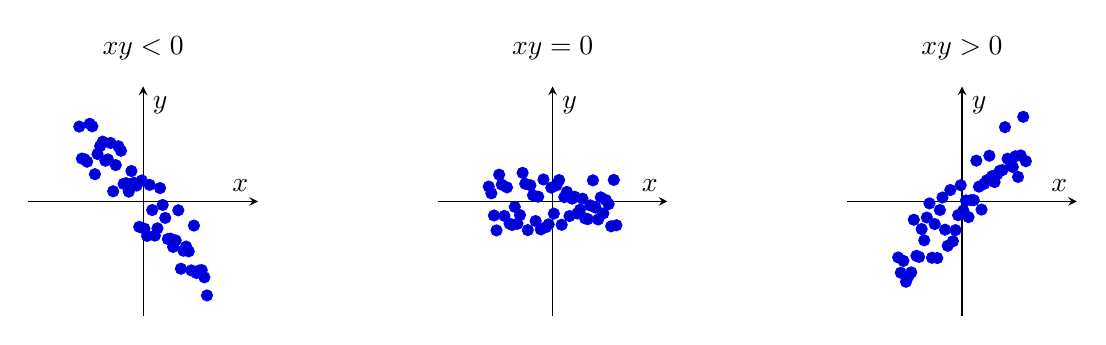
\begin{tikzpicture}
				% Covariance négative
				\begin{scope}[shift={(0,0)}]
					\begin{axis}[
						width=4.5cm, height=4.5cm,
						title={$\cov{x}{y} <0$},
						xlabel={$x$}, ylabel={$y$},
						xmin=-3, xmax=3, ymin=-3, ymax=3,
						xtick=\empty, ytick=\empty,
						axis lines=middle, enlargelimits
						]
						\addplot+[only marks, mark=*, samples=50, domain=-2:2] 
						({x}, {-x + rand});
					\end{axis}
				\end{scope}
				% Covariance nulle
				\begin{scope}[shift={(5.2cm,0)}]
					\begin{axis}[
						width=4.5cm, height=4.5cm,
						title={$\cov{x}{y} =0$}, xlabel={$x$}, ylabel={$y$},
						xmin=-3, xmax=3, ymin=-3, ymax=3,
						xtick=\empty, ytick=\empty,
						axis lines=middle, enlargelimits
						]
						\addplot+[only marks, mark=*, samples=50, domain=-2:2] 
						({x}, {rand});
					\end{axis}
				\end{scope}
				% Covariance positive
				\begin{scope}[shift={(10.4cm,0)}]
					\begin{axis}[
						width=4.5cm, height=4.5cm,
						title={$\cov{x}{y} > 0$},
						xlabel={$x$}, ylabel={$y$},
						xmin=-3, xmax=3, ymin=-3, ymax=3,
						xtick=\empty, ytick=\empty,
						axis lines=middle, enlargelimits
						]
						\addplot+[only marks, mark=*, samples=50, domain=-2:2] 
						({x}, {x + rand});
					\end{axis}
				\end{scope}
			\end{tikzpicture}
			\caption{\Glspl{scatterplot} illustrant des \glspl{realization} issues de trois \glspl{probmodel} différents pour deux \glspl{rv} avec des valeurs de covariance négative (gauche), nulle (centre) et positive (droite).}
			\label{fig:covariance-examples_dict}
		\end{figure}
	},
	first={covariance},
	text={covariance}
}

 \newglossaryentry{probspace}{
 	name={espace probabilisé}, 
 	description={Un\index{espace probabilisé} espace probabilisé est un \gls{model} mathématique d’un processus physique (une expérience aléatoire) avec un résultat incertain. Formellement, un espace probabilisé $\mathcal{P}$ est un triplet $(\Omega, \mathcal{F}, P)$ où
 		\begin{itemize} 
 			\item $\Omega$ est un espace échantillon contenant tous les résultats élémentaires possibles d’une expérience aléatoire ;
 			\item $\mathcal{F}$ est une tribu (ou sigma-algèbre), une collection de sous-ensembles de $\Omega$ (appelés événements) qui satisfait certaines propriétés de fermeture par opérations sur les ensembles ;
 			\item $P$ est une mesure de \gls{probability}, une fonction qui attribue une \gls{probability} $P(\mathcal{A}) \in [0,1]$ à chaque événement $\mathcal{A} \in \mathcal{F}$. Cette fonction doit satisfaire $P(\Omega) = 1$ et 
 			$$
 			P\left(\bigcup_{i=1}^{\infty} \mathcal{A}_i\right) = \sum_{i=1}^{\infty} P(\mathcal{A}_i)
 			$$
 			pour toute suite dénombrable d’événements deux à deux disjoints $\mathcal{A}_1, \mathcal{A}_2, \dots$ dans $\mathcal{F}$.
 		\end{itemize}
 		Les espaces probabilisés fournissent la base pour définir les \glspl{rv} et raisonner sur \gls{uncertainty} dans les applications d'\gls{ml} \cite{BillingsleyProbMeasure,GrayProbBook,ross2013first}.},
 	first={espace probabilisé}, plural={espaces probabilisés},
 	text={espace probabilisé}
 }

\newglossaryentry{realization}
{name={réalisation},
	description={Considérons\index{réalisation} une \gls{rv} $x$ qui associe à chaque élément 
		(c’est-à-dire un résultat ou événement élémentaire) $\omega \in \mathcal{P}$ d’un \gls{probspace} $\mathcal{P}$ 
		un élément $a$ d’un espace mesurable $\mathcal{N}$ \cite{BillingsleyProbMeasure,RudinBookPrinciplesMatheAnalysis,HalmosMeasure}.  
		Une réalisation de $x$ est tout élément $a' \in \mathcal{N}$ pour lequel il existe un élément 
		$\omega' \in \mathcal{P}$ tel que $x(\omega') = a'$.},
	first={réalisation}, text={réalisation}
}

\newglossaryentry{mvndist}{name ={loi normale multivariée}, 
	description={La\index{loi normale multivariée} loi normale multivariée 
		$\mvnormal{\vm}{\mC}$ est un \gls{probmodel} important pour les \glspl{featurevec} numériques. 
		C’est une famille de \glspl{probdist} pour une \gls{rv} vectorielle 
		$\featurevec \in \mathbb{R}^{\nrfeatures}$ \cite{BertsekasProb}, \cite{GrayProbBook}, \cite{Lapidoth09}. 
		Chaque membre (i.e. une \gls{probdist}) de cette famille est spécifié par sa \gls{mean} $\vm$ et 
		sa \gls{covmtx} $\mC$. Si la \gls{covmtx} est inversible, la \gls{probdist} de $\featurevec$ peut 
		s’écrire :
		$$p(\featurevec) \propto \exp\bigg(-(1/2) \big( \featurevec - \vm \big)^{T} \mC^{-1} \big( \featurevec - \vm \big) \bigg).$$
	},
	first={loi normale multivariée}, plural={lois normales multivariées}, text={loi normale multivariée}}

\newglossaryentry{covmtx}{name={matrice de covariance}, 
	description={La\index{matrice de covariance} matrice de covariance d’une \gls{rv} $\vx \in \mathbb{R}^{\featuredim}$ 
		est définie comme $\expect \bigg \{ \big( \vx - \expect \big\{ \vx \big\} \big)  \big(\vx - \expect \big\{ \vx \big\} \big)^{T} \bigg\}$.},
	first={matrice de covariance}, plural={matrices de covariance}, text={matrice de covariance} }

\newglossaryentry{gaussrv}{
	name={variable aléatoire normale centrée réduite},
	description={
		Une \index{variable aléatoire normale centrée réduite} \gls{rv} normale centrée réduite est une
		\gls{rv} réelle $x$ dont la \gls{pdf} est donnée par \cite{BertsekasProb}, \cite{GrayProbBook}, \cite{papoulis}
		\begin{equation}
			\nonumber
			p(x) = \frac{1}{\sqrt{2\pi}} \exp^{-x^2/2}. 
		\end{equation}
		Étant donnée une \gls{rv} normale centrée réduite $x$, on peut construire une \gls{rv} normale $x'$ 
		ayant pour \gls{mean} $\mu$ et \gls{variance} $\sigma^2$ via $x' \defeq \sigma (x+\mu)$. La \gls{probdist} 
		d’une \gls{rv} normale est appelée loi normale (ou loi gaussienne), notée $\mathcal{N}(\mu,\sigma)$.\\
		Un vecteur aléatoire gaussien $\featurevec \in \mathbb{R}^{\featuredim}$ ayant pour \gls{covmtx} 
		$\mathbf{C}$ et pour \gls{mean} ${\bm \mu}$ peut être construit via 
		$\featurevec \defeq \mathbf{A} \big( \vz + {\bm \mu} \big)$, où $\mA$ est une matrice telle que 
		$\mA\mA^{T} = \mC$, et $\vz \defeq \big( z_{1},\ldots,z_{\featuredim} \big)^{T}$
		est un vecteur dont les composantes sont des \gls{rv} normales centrées réduites \gls{iid} $z_{1},\ldots,z_{\featuredim}$.\\
		Les vecteurs aléatoires gaussiens constituent un cas particulier des processus gaussiens, 
		qui sont des transformations linéaires de suites infinies de \gls{rv} normales centrées réduites \cite{Rasmussen2006Gaussian}.\\
		Les \gls{rv} normales sont largement utilisées comme \glspl{probmodel} pour l’analyse statistique 
		en \gls{ml}. Leur importance provient en partie du théorème central limite, 
		qui stipule que la moyenne d’un nombre croissant de \gls{rv} indépendantes 
		(pas nécessairement normales) converge vers une \gls{rv} normale \cite{ross2013first}.\\
		Voir aussi : \gls{probdist}, \gls{probspace}.
	},
	first={variable aléatoire normale centrée réduite (VA normale centrée réduite)}, plural = {VA normales centrées réduites},
	text={VA normale centrée réduite}
}

\newglossaryentry{variance}
{
	name={variance},
	description={La\index{variance} variance d’une \gls{rv} réelle $\feature$ est définie comme l’\gls{expectation} 
		$\expect\big\{ \big( x - \expect\{x \} \big)^{2} \big\}$ de la différence au carré entre $\feature$ 
		et son \gls{expectation} $\expect\{x \}$. On étend cette définition aux \gls{rv} vectorielles $\featurevec$ 
		avec $\expect\big\{ \big\| \featurevec - \expect\{\featurevec \} \big\|_{2}^{2} \big\}$.},
	first={variance},text={variance} 
}

\newglossaryentry{mean}
{name={moyenne},
	description={La \index{moyenne} moyenne d’une \gls{rv} $\featurevec$, à valeurs dans un espace euclidien $\mathbb{R}^{\dimlocalmodel}$, est son 
		\gls{expectation} $\expect\{\featurevec\}$. Elle est définie comme l'intégrale de Lebesgue 
		de $\featurevec$ par rapport à la \gls{probdist} sous-jacente $P$,
		\[
		\expect\{\featurevec\} = \int_{\mathbb{R}^{\dimlocalmodel}} \vx \, \mathrm{d}P(\vx),
		\]
		voir par exemple \cite{BillingsleyProbMeasure} ou \cite{RudinBookPrinciplesMatheAnalysis}. 
		Nous utilisons également ce terme pour désigner la moyenne d’une séquence finie 
		$\vx^{(1)}, \ldots, \vx^{(\samplesize)} \in \mathbb{R}^{\dimlocalmodel}$. Cependant, 
		ces deux définitions sont essentiellement équivalentes. En effet, on peut utiliser la séquence 
		$\vx^{(1)}, \ldots, \vx^{(\samplesize)} \in \mathbb{R}^{\dimlocalmodel}$ pour construire une 
		\gls{rv} discrète $\widetilde{\vx}=\vx^{(I)}$ où l’indice $I$ est choisi uniformément 
		au hasard dans l’ensemble $\{1,\ldots,\samplesize\}$. La moyenne de $\widetilde{\vx}$ est 
		précisément la moyenne empirique $\frac{1}{\samplesize} \sum_{\sampleidx=1}^{\samplesize} \vx^{(\sampleidx)}$.},
	first={moyenne}, text={moyenne}
}

\newglossaryentry{dataset}{
	name={jeu de données},
	description={
		Un\index{jeu de données} jeu de données désigne une collection de \glspl{datapoint}. Ces 
		\glspl{datapoint} portent des informations sur une certaine quantité d’intérêt (ou \gls{label}) 
		dans une application de l'\gls{ml}. Les méthodes d'\gls{ml} utilisent des jeux de données pour 
		l'entraînement du \gls{model} (par exemple via la \gls{erm}) et la \gls{validation} du \gls{model}.\\
		Il est important de noter que notre notion de jeu de données est très flexible, car elle autorise 
		des types de \glspl{datapoint} très variés. En effet, les \glspl{datapoint} peuvent être des objets physiques 
		concrets (comme des humains ou des animaux) ou des objets abstraits (comme des nombres).\\
		À titre d'exemple, la Figure~\ref{fig_cows_dataset} illustre un jeu de données utilisant des vaches 
		comme \glspl{datapoint}.
		\begin{figure}[H]
			\begin{center}
				\label{fig:cowsintheswissalps_dict}
				\includegraphics[width=0.5\textwidth]{../../assets/CowsAustria.jpg}
			\end{center}
			\caption{\label{fig_cows_dataset_dict}Un troupeau de vaches dans les Alpes}
		\end{figure}
		Bien souvent, un ingénieur en \gls{ml} n’a pas d’accès direct à un jeu de données. En effet, 
		accéder au jeu de données de la Figure~\ref{fig_cows_dataset} impliquerait de visiter le troupeau 
		de vaches dans les Alpes. À la place, il faut utiliser une approximation (ou représentation) du jeu de données 
		plus pratique à manipuler.\\
		Divers modèles mathématiques ont été développés pour représenter ou approximer les jeux de données 
		\cite{silberschatz2019database}, \cite{abiteboul1995foundations}, \cite{hoberman2009data}, 
		\cite{ramakrishnan2002database}.\\
		L’un des \glspl{model} de \gls{data} les plus utilisés est le modèle relationnel, 
		qui organise les données sous forme de tableau (ou relation) \cite{codd1970relational}, 
		\cite{silberschatz2019database}.\\
		Un tableau est composé de lignes et de colonnes :
		\begin{itemize}
			\item Chaque ligne du tableau représente un seul \gls{datapoint}.
			\item Chaque colonne du tableau correspond à un attribut spécifique du \gls{datapoint}. 
			Les méthodes d'\gls{ml} peuvent utiliser ces attributs comme \glspl{feature} ou \glspl{label}
			du \gls{datapoint}.
		\end{itemize}
		Par exemple, la Table~\ref{tab:cowdata} montre une représentation du jeu de données de la Figure~\ref{fig_cows_dataset}.
		Dans le \gls{model} relationnel, l’ordre des lignes est sans importance, et chaque attribut 
		(colonne) doit être défini précisément par un domaine spécifiant l’ensemble des valeurs possibles.\\
		Dans les applications de l'\gls{ml}, ces domaines d’attributs deviennent l’\gls{featurespace} 
		et l'\gls{labelspace}.
		\begin{table}[H]
			\centering
			\begin{tabular}{lcccc}
				\hline
				\textbf{Nom} & \textbf{Poids} & \textbf{Âge} & \textbf{Taille} & \textbf{Température de l'estomac} \\
				\hline
				Zenzi & 100 & 4 & 100 & 25 \\
				Berta & 140 & 3 & 130 & 23 \\
				Resi  & 120 & 4 & 120 & 31 \\
				\hline
			\end{tabular}
			\caption{Une relation (ou table) représentant le jeu de données de la Figure~\ref{fig_cows_dataset}.}
			\label{tab:cowdata}
		\end{table}
		Bien que le modèle relationnel soit utile pour de nombreuses applications en \gls{ml}, 
		il peut s’avérer insuffisant vis-à-vis des exigences en matière de \gls{trustAI}.\\
		Des approches modernes, telles que les fiches descriptives des jeux de données, proposent une documentation 
		plus complète, incluant des détails sur le processus de collecte des données, l’usage prévu 
		et d’autres informations contextuelles \cite{DatasheetData2021}.
	},
	first={jeu de données},
	text={jeu de données},
	plural={jeux de données}
}

\newglossaryentry{featurevec}
{name={vecteur de caractéristiques},
	description={Un \index{vecteur de caractéristiques} vecteur de \glspl{feature} est un vecteur 
		$\vx = \big(x_{1},\ldots,x_{\nrfeatures}\big)^{T}$ dont les composantes sont des \glspl{feature} individuelles 
		$x_{1},\ldots,x_{\nrfeatures}$. De nombreuses méthodes d'\gls{ml} utilisent des vecteurs de \glspl{feature} 
		appartenant à un \gls{euclidspace} de dimension finie $\mathbb{R}^{\nrfeatures}$. 
		Cependant, pour certaines méthodes d'\gls{ml}, il peut être plus pratique de travailler avec des 
		vecteurs de \glspl{feature} appartenant à un espace vectoriel de dimension infinie 
		(par exemple, voir la \gls{kernelmethod}).},
	first={vecteur de caractéristiques},
	text={vecteur de caractéristiques},
	plural={vecteurs de caractéristiques}
}

\newglossaryentry{featurespace}
{name={espace des caractéristiques},
	description={
		L’\index{espace des caractéristiques}espace des \glspl{feature} d’une application ou méthode d'\gls{ml} 
		correspond à l’ensemble de toutes les valeurs possibles que peut prendre le \gls{featurevec} 
		d’un \gls{datapoint}. Un choix largement utilisé pour l’espace des \glspl{feature} est l’\gls{euclidspace} 
		$\mathbb{R}^{\featuredim}$, où la dimension $\featurelen$ représente le nombre de \glspl{feature} individuelles 
		d’un \gls{datapoint}.},
	first={espace des caractéristiques},
	text={espace des caractéristiques}, plural = {espaces des caractéristiques}
}

\newglossaryentry{regression}
{name={régression},
	description={Les problèmes de régression\index{régression} se concentrent sur la prédiction d'une \gls{label} numérique uniquement à partir des \glspl{feature} d'un \gls{datapoint} \cite[Ch. 2]{MLBasics}.},
	first={régression},text={régression} 
}

\newglossaryentry{trainset}
{name={ensemble d'entraînement (ou d'apprentissage)},
	description={Un\index{ensemble d'entraînement (ou d'apprentissage)} ensemble d'entraînement est un \gls{dataset} $\dataset$ composé de certains \glspl{datapoint} utilisés dans le cadre d'une \gls{erm} 
		pour apprendre une \gls{hypothesis} $\learnthypothesis$. La \gls{loss} moyenne de $\learnthypothesis$ sur 
		l'ensemble d'entraînement est appelée \gls{trainerr}. La comparaison entre l'\gls{trainerr} et l'\gls{valerr} de $\learnthypothesis$ permet de évaluer la qualité de la méthode d'\gls{ml} utilisée et fournit des indications 
		pour améliorer l'erreur de validation (par exemple, en utilisant un autre \gls{hypospace} ou en collectant plus de \glspl{datapoint}) \cite[Sec. 6.6]{MLBasics}.},first={ensemble d'entraînement (ou d'apprentissage)},text={ensemble d'entraînement}, plural={ensembles d'entraînement}  
}

\newglossaryentry{classification}
{name={classification},
	description={La classification\index{classification} est la tâche qui consiste à déterminer une étiquette discrète $\truelabel$ pour un \gls{datapoint} donné, uniquement à partir de ses \glspl{feature}. L'étiquette $\truelabel$ appartient à un ensemble fini, par exemple $\truelabel \in \{-1,1\}$ ou $\truelabel \in \{1,\ldots,19\}$, et représente la catégorie à laquelle appartient le \gls{datapoint} correspondant.},
	first={classification},text={classification} 
}

\newglossaryentry{batch}
{
	name={lot},
	description={Dans\index{lot} le contexte de la \gls{stochGD}, un lot désigne un sous-ensemble choisi aléatoirement dans l’\gls{trainset} complet. On utilise les \glspl{datapoint} de ce sous-ensemble pour estimer le \gls{gradient} de l’\gls{trainerr} et, par la suite, mettre à jour les \gls{modelparams}.}, 
	first={lot},text={lot}  
}

\newglossaryentry{hypothesis}
{name={hypothèse},
	description={Une\index{hypothèse} hypothèse désigne une application (ou fonction) $\hypothesis: \featurespace \rightarrow \labelspace$ allant de l'\gls{featurespace} $\featurespace$ vers l'\gls{labelspace} $\labelspace$. 
		Étant donné un \gls{datapoint} avec des \glspl{feature} $\featurevec$, on utilise une fonction hypothèse $\hypothesis$
		pour estimer (ou approximer) son \gls{label} $\truelabel$ à l’aide de la \gls{prediction}  
		$\hat{\truelabel} = \hypothesis(\featurevec)$. L’\gls{ml} consiste à apprendre (ou trouver) une 
		hypothèse $\hypothesis$ telle que $\truelabel \approx \hypothesis(\featurevec)$ 
		pour tout \gls{datapoint} (de \glspl{feature} $\featurevec$ et \gls{label} $\truelabel$).},
	first={hypothèse}, text={hypothèse}
}

\newglossaryentry{hypospace}{
	name={espace des hypothèses},
	description={Toute méthode pratique d’\gls{ml} utilise un espace des hypothèses (ou \gls{model}) $\hypospace$. L’espace des hypothèses d’une méthode d’\gls{ml} est un sous-ensemble de l'ensemble des applications allant de l’\gls{featurespace} dans l’\gls{labelspace}. Le choix de cet espace doit tenir compte des ressources informatiques disponibles ainsi que des \gls{statasp}. Si l’infrastructure permet des opérations matricielles efficaces, et qu’il existe une relation (approximativement) linéaire entre un ensemble de \glspl{feature} et une \gls{label}, un choix pertinent pour l’espace des hypothèses peut être un \gls{linmodel}.},
	first={espace des hypothèses},
	text={espace des hypothèses} 
}

\newglossaryentry{model}{
	name={modèle},
	description={Dans\index{modèle} le contexte de l’\gls{ml}, le terme « modèle » désigne typiquement l’\gls{hypospace} sous-jacent à une méthode d’\gls{ml} \cite{MLBasics}, \cite{ShalevMLBook}. Cependant, ce terme est également utilisé dans d’autres domaines avec des significations différentes. Par exemple, un \gls{probmodel} désigne un ensemble paramétré de \glspl{probdist}.},
	first={modèle},
	text={modèle} 
}

\newglossaryentry{effdim}
{name={dimension effective},
	description={La\index{dimension effective} dimension effective $\effdim{\hypospace}$ d’un \gls{hypospace} infini $\hypospace$ est une mesure de sa taille. Grosso modo, la dimension effective correspond au nombre effectif de \gls{modelparams} ajustables indépendants. Ces \gls{parameters} peuvent être les coefficients utilisés dans une application linéaire ou les \glspl{weights} et termes de biais d’un \gls{ann}.},
	first={dimension effective},
	text={dimension effective}  
}

\newglossaryentry{bias}
{
	name={biais},
	description={Considérons\index{biais} une méthode d'\gls{ml} utilisant un \gls{hypospace} paramétré $\hypospace$. 
		Celle-ci apprend les \gls{modelparams} $\weights \in \mathbb{R}^{\dimlocalmodel}$ à partir du \gls{dataset} 
		$$ \dataset=\big\{ \pair{\featurevec^{(\sampleidx)}}{\truelabel^{(\sampleidx)}} \big\}_{\sampleidx=1}^{\samplesize}.$$ 
		Pour analyser les propriétés de la méthode d'\gls{ml}, on interprète généralement les \glspl{datapoint} comme des \glspl{realization} de
		\gls{rv} \gls{iid}), 
		$$ \truelabel^{(\sampleidx)} = \hypothesis^{(\overline{\weights})}\big( \featurevec^{(\sampleidx)} \big) + \bm{\varepsilon}^{(\sampleidx)}, \quad \sampleidx=1,\ldots,\samplesize.$$ 
		On peut alors considérer la méthode d'\gls{ml} comme un estimateur $\widehat{\weights}$ 
		calculé à partir de $\dataset$ (par exemple, en résolvant une \gls{erm}). Le biais (au carré) de l’estimateur $\widehat{\weights}$ 
		se définit alors comme $\biasterm^{2} \defeq \big\| \expect \{ \widehat{\weights}  \}- \overline{\weights}\big\|_{2}^{2}$.},
	first={biais},text={biais} 
}

\newglossaryentry{data}
{name={données},
	description={Les\index{données} données désignent des objets porteurs d'information. Ces objets peuvent être des entités physiques concrètes (comme des personnes ou des animaux), ou des concepts abstraits (comme des nombres). On utilise souvent des représentations (ou des approximations) des données originales, plus pratiques pour le traitement. Ces approximations reposent sur différents \glspl{model} de données, le modèle relationnel étant l’un des plus utilisés \cite{codd1970relational}.}, 
	text={données}
}

\newglossaryentry{parameters}{
	name={paramètres},
	description={Les\index{paramètres} paramètres d’un \gls{model} en \gls{ml} sont des quantités ajustables 
		(c’est-à-dire apprenables ou modifiables) qui permettent de choisir parmi différentes fonctions \gls{hypothesis}. 
		Par exemple, le \gls{linmodel} $\hypospace \defeq \{\hypothesis^{(\weights)}: \hypothesis^{(\weights)}(\feature)= \weight_{1} \feature + \weight_{2}\}$ 
		correspond à l’ensemble des fonctions \gls{hypothesis} $\hypothesis^{(\weights)}(\feature)= \weight_{1} \feature + \weight_{2}$ 
		avec un choix particulier des paramètres $\weights = \big(\weight_{1},\weight_{2}\big)^{T} \in \mathbb{R}^{2}$. 
		Un autre exemple de paramètres est le \gls{weights} attribué à une connexion entre deux neurones dans un \gls{ann}.},
	first={paramètres},text={paramètres}
}

\newglossaryentry{loss}{
	name={perte (ou coût)},
	description={En \gls{ml}\index{perte (ou coût)}, on utilise une \gls{lossfunc} $\lossfunc{\datapoint}{\hypothesis}$ pour mesurer l’erreur commise lorsqu’une \gls{hypothesis} est appliquée à une \gls{datapoint}. Par léger abus de langage, on utilise le terme \emph{perte} à la fois pour désigner la fonction de perte $\loss$ elle-même et la valeur spécifique $\lossfunc{\datapoint}{\hypothesis}$ associée à une donnée $\datapoint$ et une hypothèse $\hypothesis$.},
	first={perte},
	text={perte}
}

\newglossaryentry{valset}{
	name={ensemble de validation (ou jeu de validation)},
	description={Un\index{ensemble de validation (ou jeu de validation)} ensemble de \glspl{datapoint} utilisé pour estimer 
		le \gls{risk} d'une \gls{hypothesis} $\learnthypothesis$ apprise par une méthode 
		d'\gls{ml} (par exemple, par résolution d’un problème de \gls{erm}). La \gls{loss} 
		moyenne de $\learnthypothesis$ sur l’ensemble de validation est appelée \gls{valerr} 
		et peut servir à évaluer les performances d'une méthode d'apprentissage 
		(voir \cite[Sec. 6.6]{MLBasics}). La comparaison entre \gls{trainerr} et \gls{valerr} 
		peut guider des améliorations de la méthode (telles que le choix d’un autre \gls{hypospace}).},
	first={ensemble de validation},
	text={ensemble de validation}, plural ={ensembles de validation}
}

\newglossaryentry{valerr}{
	name={erreur de validation},
	description={Considérons\index{erreur de validation} une \gls{hypothesis} $\learnthypothesis$ obtenue à l'aide d'une 
		méthode d'\gls{ml}, par exemple en résolvant un problème de \gls{erm} sur un \gls{trainset}. 
		La \gls{loss} moyenne de $\learnthypothesis$ sur un \gls{valset}, distinct de l'ensemble d'entraînement, 
		est appelée erreur de validation.},
	first={erreur de validation}, plural ={erreurs de validation},
	text={erreur de validation}
}

\newglossaryentry{emprisk}
{name={risque empirique},
	description={Le \gls{risk}\index{risque empirique} empirique $\emprisk{\hypothesis}{\dataset}$ 
		d’une \gls{hypothesis} sur un \gls{dataset} $\dataset$ correspond à la \gls{loss} moyenne
		encourue par $\hypothesis$ lorsqu’elle est appliquée aux différents \glspl{datapoint} 
		de $\dataset$.},
	first={risque empirique}, text={risque empirique} , plural={risques empiriques}
}

\newglossaryentry{trainerr}
{
	name={erreur d'entrainement},
	description={La\index{erreur d'entrainement} \gls{loss} moyenne d’une \gls{hypothesis} lors de 
		la prédiction des \glspl{label} des \glspl{datapoint} dans un \gls{trainset}. 
		On désigne parfois aussi par erreur d’entraînement la \gls{loss} moyenne minimale 
		qui est atteinte par une solution de \gls{erm}.},
	first={erreur d'entrainement}, text={erreur d'entrainement} , plural = {erreurs d'entrainement} 
}

\newglossaryentry{regularization}{
	name={régularisation},
	description={
		Un\index{régularisation} défi majeur des applications modernes d'\gls{ml} est qu’elles utilisent souvent de grands \glspl{model}, avec une \gls{effdim} de l’ordre du milliard. 
		Entraîner un \gls{model} de grande dimension à l’aide de méthodes de \gls{erm} basiques conduit souvent au \gls{overfitting} : l’\gls{hypothesis} apprise a de bonnes performances sur l' \gls{trainset} 
		mais insuffisantes en dehors de celui-ci. La régularisation désigne des modifications apportées à une instance donnée de \gls{erm} afin d’éviter le \gls{overfitting}, c’est-à-dire pour garantir que l’\gls{hypothesis} apprise fonctionne 
		presque aussi bien en dehors de l'\gls{trainset}. Il existe trois manières de mettre en œuvre la régularisation :
		\begin{enumerate}[label=\arabic*)]
			\item {Élaguer le \gls{model} :} on réduit le \gls{model} original $\hypospace$ pour obtenir un 
			\gls{model} plus petit $\hypospace'$. Dans le cas d'un \gls{model} paramétrique, cette réduction peut se faire 
			via des contraintes sur les \gls{modelparams} (par exemple $w_{1} \in [0.4,0.6]$ pour 
			le poids de la \gls{feature} $x_{1}$ dans la \gls{linreg}).
			\item {Pénaliser la \gls{loss} :} on modifie la \gls{objfunc} de la \gls{erm} en ajoutant un 
			terme de pénalité à l’\gls{trainerr}. Ce terme estime combien la \gls{loss} (ou le \gls{risk}) attendue est plus grande 
			que la \gls{loss} moyenne sur l'\gls{trainset}.
			\item {\Gls{dataaug} :} on peut agrandir l'\gls{trainset} $\dataset$ en ajoutant 
			des copies perturbées des \glspl{datapoint} originaux de $\dataset$. Une telle 
			perturbation consiste par exemple à ajouter la \gls{realization} d’une \gls{rv} au \gls{featurevec} 
			d’un \gls{datapoint}.
		\end{enumerate}
		La figure \ref{fig_equiv_dataaug_penal_dict} illustre ces trois approches de régularisation. 
		Ces approches sont étroitement liées et parfois entièrement équivalentes : la \gls{dataaug} qui utilise des \glspl{gaussrv} 
		pour perturber les \glspl{featurevec} de l'\gls{trainset} dans le cas de la \gls{linreg} 
		a le même effet que l’ajout du terme de pénalité 
		$\lambda \normgeneric{\weights}{2}^2$ à l’\gls{trainerr} (ce qui correspond à la \gls{ridgeregression}). 
		Le choix de la méthode de régularisation peut dépendre des ressources de calcul disponibles. Par exemple, il peut être bien plus facile de 
		mettre en œuvre une \gls{dataaug} que de réaliser un élagage de \gls{model}. 
		\begin{figure}[H]
			\begin{center} 
				\begin{tikzpicture}[scale = 1]
					% Axes
					\draw[->, very thick] (0,0.5) -- (7.7,0.5) node[right] {\gls{feature} $\feature$};       % X-axis
					\draw[->, very thick] (0.5,0) -- (0.5,4.2) node[above] {\gls{label} $\truelabel$};   % Y-axis
					\draw[color=black, thick, dashed, domain = -1: 6.2, variable = \x]  plot ({\x},{\x*0.4 + 2.0}) ;     
					\draw[color=black, thick, dashed, domain = -1: 6.2, variable = \x]  plot ({\x},{\x*0.6 + 2.0}) ;     
					% Add a lasso around the two dashed lines
					% Ellipse around the two dashed lines
					\draw[blue, thick] (5, 4.5) ellipse [x radius=0.2cm, y radius=1cm];
					\node at (5, 5.8) [text=black, font=\small] {$\{ \hypothesis: \hypothesis(x)\!=\!w_{1}x\!+\!w_{0}; w_{1} \in [0.4,0.6]\}$};
					\node at (6.7,4.5) {$\hypothesis(\feature)$};    
					\coordinate (l1)   at (1.2, 2.48);
					\coordinate (l2) at (1.4, 2.56);
					\coordinate (l3)   at (1.7,  2.68);
					\coordinate (l4)   at (2.2, 2.2*0.4+2.0);
					\coordinate (l5) at (2.4, 2.4*0.4+2.0);
					\coordinate (l6)   at (2.7,  2.7*0.4+2.0);
					\coordinate (l7)   at (3.9,  3.9*0.4+2.0);
					\coordinate (l8) at (4.2, 4.2*0.4+2.0);
					\coordinate (l9)   at (4.5,  4.5*0.4+2.0);
					\coordinate (n1)   at (1.2, 1.8);
					\coordinate (n2) at (1.4, 1.8);
					\coordinate (n3)   at (1.7,  1.8);
					\coordinate (n4)   at (2.2, 3.8);
					\coordinate (n5) at (2.4, 3.8);
					\coordinate (n6)   at (2.7,  3.8);
					% augemented data point obtained by perturbing feature, not touching label value 
					\coordinate (n7)   at (3.9, 2.6);
					\coordinate (n8) at (4.2, 2.6);
					\coordinate (n9)   at (4.5,  2.6);
					\node at (n1)  [circle,draw,fill=red,minimum size=6pt,scale=0.6, name=c1] {};
					\node at (n2)  [circle,draw,fill=blue,minimum size=6pt, scale=0.6, name=c2] {};
					\node at (n3)  [circle,draw,fill=red,minimum size=6pt,scale=0.6,  name=c3] {};
					\node at (n4)  [circle,draw,fill=red,minimum size=12pt, scale=0.6, name=c4] {};  
					\node at (n5)  [circle,draw,fill=blue,minimum size=12pt,scale=0.6,  name=c5] {};
					\node at (n6)  [circle,draw,fill=red,minimum size=12pt, scale=0.6, name=c6] {};  
					\node at (n7)  [circle,draw,fill=red,minimum size=12pt,scale=0.6,  name=c7] {};
					\node at (n8)  [circle,draw,fill=blue,minimum size=12pt, scale=0.6, name=c8] {};
					\node at (n9)  [circle,draw,fill=red,minimum size=12pt, scale=0.6, name=c9] {};
					\draw [<->] ($ (n7) + (0,-0.3) $)  --  ($ (n9) + (0,-0.3) $) node [pos=0.4, below] {$\sqrt{\regparam}$}; ; 
					\draw[<->, color=red, thick] (l1) -- (c1);  
					\draw[<->, color=blue, thick] (l2) -- (c2);  
					\draw[<->, color=red, thick] (l3) -- (c3);  
					\draw[<->, color=red, thick] (l4) -- (c4);  
					\draw[<->, color=blue, thick] (l5) -- (c5);  
					\draw[<->, color=red, thick] (l6) -- (c6);  
					\draw[<->, color=red, thick] (l7) -- (c7);  
					\draw[<->, color=blue, thick] (l8) -- (c8);  
					\draw[<->, color=red, thick] (l9) -- (c9);  
					\draw[fill=blue] (6.2, 3.7)  circle (0.1cm) node [black,xshift=3.6cm] {\gls{trainset} original $\dataset$};
					\draw[fill=red] (6.2, 3.2)  circle (0.1cm) node [black,xshift=1.3cm] {augmenté};
					\node at (4.6,1.2)  [minimum size=12pt, font=\fontsize{12}{0}\selectfont, text=blue] {$\frac{1}{\samplesize} \sum_{\sampleidx=1}^\samplesize \lossfunc{\pair{\featurevec^{(\sampleidx)}}{ \truelabel^{(\sampleidx)}}}{\hypothesis}$};
					\node at (7.8,1.2)  [minimum size=12pt, font=\fontsize{12}{0}\selectfont, text=red] {$+\regparam \regularizer{\hypothesis}$};
				\end{tikzpicture}
				\caption{Trois approches pour la régularisation: 1) \gls{dataaug}; 2) pénalisation de la perte; et 3) élagage du \gls{model} (via des contraintes sur les \gls{modelparams}). \label{fig_equiv_dataaug_penal_dict} }
			\end{center}
		\end{figure}
	},
	first={régularisation},
	text={régularisation}
}

\newglossaryentry{learningtask}{
	name={tâche d'apprentissage},
	description={
		Considérons\index{tâche d'apprentissage} un \gls{dataset} $\dataset$ constitué de plusieurs \glspl{datapoint}, chacun étant caractérisé par des \glspl{feature} $\featurevec$. Par exemple, le \gls{dataset} $\dataset$ peut être constitué des images d’une base de données particulière. Parfois, il peut être utile de représenter un \gls{dataset} $\dataset$, ainsi que le choix des \glspl{feature}, par une \gls{probdist} $p(\featurevec)$. Une tâche d'apprentissage associée à $\dataset$ consiste en un choix spécifique pour l'\gls{label} d’un \gls{datapoint} et l’\gls{labelspace} correspondant. Étant donné un choix de \gls{lossfunc} et de \gls{model}, une tâche d’apprentissage donne lieu à une instance de \gls{erm}. Ainsi, on pourrait aussi définir une tâche d’apprentissage via une instance de \gls{erm}, c’est-à-dire via une \gls{objfunc}. Remarquons que, pour un même \gls{dataset}, on obtient différentes tâches d’apprentissage en utilisant différents choix de \glspl{feature} et d'\gls{label} d’un \gls{datapoint}. Ces tâches d’apprentissage sont liées, puisqu’elles sont basées sur le même \gls{dataset}, et les résoudre conjointement (via des méthodes de \gls{multitask learning}) est en général préférable à des résolutions distinctes \cite{Caruana:1997wk}, \cite{JungGaphLassoSPL}, \cite{CSGraphSelJournal}.
	},
	text={tâche d'apprentissage},
	plural={tâches d'apprentissage}, plural = {tâches d'apprentissage}
}

\newglossaryentry{multitask learning}{
	name={apprentissage multitâche},
	description={
		L’apprentissage multitâche\index{apprentissage multitâche} vise à exploiter les relations entre différentes \glspl{learningtask}. 
		Considérons deux \glspl{learningtask} obtenues à partir du même \gls{dataset} d’images de webcam. 
		La première tâche consiste à prédire la présence d’un humain, tandis que la seconde tâche consiste à prédire la présence d’une voiture. 
		Il peut être utile d’utiliser la même structure de \gls{deepnet} pour les deux tâches et de ne permettre qu'aux \gls{weights} de la couche de sortie finale d’être différents.
	},
	first={apprentissage multitâche},
	text={apprentissage multitâche}, plural ={apprentissages multitâche}
}

\newglossaryentry{learnrate}{
	name={taux d'apprentissage},
	description={
		Considérons\index{taux d'apprentissage} une méthode itérative d'\gls{ml} pour trouver ou apprendre une \gls{hypothesis} utile $\hypothesis \in \hypospace$. 
		Une telle méthode itérative répète des étapes computationnelles (de mise à jour) similaires qui ajustent ou modifient 
		l’\gls{hypothesis} actuelle afin d’obtenir une \gls{hypothesis} améliorée. Un exemple bien connu de cette méthode itérative 
		est la \gls{gd} et ses variantes, \gls{stochGD} et \gls{projgd}. Un paramètre clé d’une méthode itérative est le taux d’apprentissage. 
		Le taux d’apprentissage contrôle l’ampleur selon laquelle l’\gls{hypothesis} courante peut être modifiée durant une seule itération. 
		Un exemple bien connu de tel paramètre est la \gls{stepsize} utilisée lors d'une \gls{gd} \cite[Ch. 5]{MLBasics}.
	},
	first={taux d'apprentissage},
	text={taux d'apprentissage}, plural={taux d'apprentissage}
}

\newglossaryentry{stepsize}{name={taille de pas}, description={
		Voir \index{taille de pas} \gls{learnrate}.}, 
	first={taille de pas},text={taille de pas}, plural={tailles de pas} }

\newglossaryentry{gdmethods}{
	name={méthodes basées sur le gradient},
	description={
		Les méthodes basées sur le \gls{gradient} \index{méthodes basées sur le gradient} sont des techniques itératives pour trouver le \gls{minimum} (ou le \gls{maximum}) 
		d’une \gls{objfunc} des \gls{modelparams} \gls{differentiable}. Ces méthodes construisent une suite d’approximations 
		d’un choix optimal des \gls{modelparams} qui aboutit à une valeur \gls{minimum} (ou \gls{maximum}) de la \gls{objfunc}. 
		Comme leur nom l’indique, les méthodes basées sur le \gls{gradient} utilisent les \glspl{gradient} de la \gls{objfunc} 
		évalués lors des itérations précédentes pour construire de nouveaux \gls{modelparams} (espérons-le) améliorés. 
		Un exemple important d’une méthode basée sur le \gls{gradient} est la \gls{gd}.
	},
	first={méthodes basées sur le gradient},
	text={méthodes basées sur le gradient}
}

\newglossaryentry{eigenvalue}{
	name={valeur propre},
	description={
		On qualifie\index{valeur propre} de valeur propre d'une matrice carrée $\mathbf{A} \in \mathbb{R}^{\featuredim \times \featuredim}$ 
		le nombre $\lambda \in \mathbb{R}$ s’il existe un vecteur non nul $\vx \in \mathbb{R}^{\featuredim} \setminus \{ \mathbf{0} \}$ 
		tels que $\mathbf{A} \vx = \lambda \vx$.
	},
	first={valeur propre},
	plural={valeurs propres},
	text={valeur propre}
}

\newglossaryentry{psd}
{name={semi-définie positive},
	description={
		Une matrice symétrique (à valeurs réelles) $\mQ = \mQ^{T} \in \mathbb{R}^{\featuredim \times \featuredim}$ 
		est dite semi-définie positive\index{semi-définie positive} si $\featurevec^{T} \mQ \featurevec \geq 0$ pour tout vecteur $\featurevec \in \mathbb{R}^{\featuredim}$. 
		La propriété d’être semi-définie positive peut être étendue des matrices aux applications \gls{kernel} symétriques (à valeurs réelles) 
		$\kernel: \featurespace \times \featurespace \rightarrow \mathbb{R}$ (avec $\kernel(\featurevec,\featurevec') = \kernel(\featurevec',\featurevec)$)
		de la manière suivante : pour tout ensemble fini de \glspl{featurevec} $\featurevec^{(1)},\dots,\featurevec^{(\samplesize)}$, 
		la matrice résultante $\mQ \in \mathbb{R}^{\samplesize \times \samplesize}$ avec pour coefficients  
		$Q_{\sampleidx,\sampleidx'} = \kernelmap{\featurevec^{(\sampleidx)}}{\featurevec^{(\sampleidx')}}$ 
		est semi-définie positive \cite{LearningKernelsBook}.
	},
	first={semi-définie positive},text={semi-définie positive}, plural={semi-définies positives}
}

\newglossaryentry{actfun}
{name={fonction d'activation},
	description={On associe à chaque\index{fonction d'activation} neurone artificiel dans un \gls{ann} 
		une fonction d'activation $\actfun(\cdot)$ qui prend en entrée une combinaison pondérée 
		des entrées du neurone $\feature_{1},\ldots,\feature_{\nrfeatures}$ et produit une 
		sortie unique $a = \actfun\big(\weight_{1} \feature_{1}+\ldots+\weight_{\nrfeatures} \feature_{\nrfeatures} \big)$. 
		Notons que chaque neurone est paramétré par les \gls{weights} $\weight_{1},\ldots,\weight_{\nrfeatures}$.},
	first={fonction d'activation},text={fonction d'activation} , plural={fonctions d'activation}
}

\newglossaryentry{ann}{
	name={réseau de neurones artificiels (RNA)},
	description={Un\index{réseau de neurones artificiels (RNA)} RNA 
		est une représentation graphique (circulation de signaux) d'une fonction qui associe 
		les \glspl{feature} d’un \gls{datapoint} en entrée à une \gls{prediction} 
		de l’\gls{label} correspondante en sortie. L’unité fondamentale d’un 
		RNA est le neurone artificiel, qui applique une \gls{actfun} à ses 
		entrées pondérées. Les sorties de ces neurones servent d’entrées à d’autres neurones, 
		formant des couches interconnectées.},
	first={réseau de neurones artificiels (RNA)}, plural={RNA},
	text={RNA}
}

\newglossaryentry{decisionregion}{name={région de décision}, description={Considérons\index{région de décision} 
		une fonction \gls{hypothesis} qui renvoie des valeurs d'un ensemble fini $\labelspace$. 
		Pour chaque valeur (catégorie) d'\gls{label} $a \in \labelspace$, l’\gls{hypothesis} $\hypothesis$ 
		détermine un sous-ensemble de valeurs de \glspl{feature} $\featurevec \in \featurespace$ 
		telles que $\hypothesis(\featurevec)=a$. On appelle ce sous-ensemble une région de décision 
		de l’\gls{hypothesis} $\hypothesis$.},first={région de décision},text={région de décision}, plural= {régions de décision} }
	
\newglossaryentry{weights}{name={poids},
	description={Considérons\index{poids} un \gls{hypospace} paramétré $\hypospace$. 
		On\index{weights} utilise le terme poids pour désigner des \gls{modelparams} numériques 
		utilisés pour pondérer les \glspl{feature} ou leurs transformations afin de calculer $\hypothesis^{(\weights)} \in \hypospace$. 
		Un \gls{linmodel} utilise des poids $\weights=\big(\weight_{1},\ldots,\weight_{\nrfeatures}\big)^{T}$ pour calculer 
		la combinaison linéaire $\hypothesis^{(\weights)}(\featurevec)= \weights^{T} \featurevec$. 
		Les poids sont également utilisés dans les \gls{ann} pour former des combinaisons linéaires de \glspl{feature} ou des sorties de neurones dans les couches cachées.},first={poids},text={poids}, plural={poids}}

\newglossaryentry{linmodel}{name={modèle linéaire},
	description={Considérons\index{modèle linéaire} des \glspl{datapoint}, chacun étant caractérisé par un \gls{featurevec} numérique 
		$\featurevec \in \mathbb{R}^{\featuredim}$. Un \gls{model} linéaire est 
		un \gls{hypospace} constitué de toutes les applications linéaires, 
		\begin{equation} 
			\label{equ_def_lin_model_hypspace_dict}
			\linmodel{\nrfeatures} \defeq \left\{ \hypothesis(\featurevec)= \weights^{T} \featurevec: \weights \in \mathbb{R}^{\nrfeatures} \right\}. 
		\end{equation} 
		Notons que \eqref{equ_def_lin_model_hypspace_dict} définit une famille entière d'\glspl{hypospace}, 
		paramétrée par le nombre $\nrfeatures$ de \glspl{feature} qui sont combinées linéairement pour former la 
		\gls{prediction} $\hypothesis(\featurevec)$. Le choix de $\nrfeatures$ est guidé par les 
		\gls{compasp} (par exemple, réduire $\nrfeatures$ signifie moins de calcul), les \gls{statasp} 
		(par exemple, augmenter $\nrfeatures$ peut réduire l’erreur de \gls{prediction}) et 
		l’\gls{interpretability}. Un \gls{model} linéaire utilisant peu de \glspl{feature} soigneusement sélectionnées 
		a tendance à être considéré comme plus interprétable \cite{Ribeiro2016,rudin2019stop}.}, 
	first={modèle linéaire},text={modèle linéaire}, plural={modèles linéaires}}

\newglossaryentry{modelparams}{name={paramètres du modèle}, 
	description={Les \gls{parameters} d’un \gls{model}\index{paramètres du modèle} sont des quantités 
		utilisées pour sélectionner une fonction \gls{hypothesis} spécifique à partir d’un \gls{model}. 
		On peut considérer une liste de \gls{parameters} de \gls{model} comme un identifiant unique 
		d’une fonction \gls{hypothesis}, de la même manière qu’un numéro de sécurité sociale 
		identifie une personne en France.},
	first={paramètres du modèle},text={paramètres du modèle} }

\newglossaryentry{featuremap}{
	name={transformation de caractéristiques},
	description={
		Un trasnformation  de \glspl{feature} \index{transformation de caractéristiques} est une application qui transforme les \glspl{feature} originales d’un \gls{datapoint} en de nouvelles \glspl{feature}. 
		Les nouvelles \glspl{feature} obtenues peuvent être préférables aux \glspl{feature} d’origine pour plusieurs raisons. 
		Par exemple, l’agencement des \glspl{datapoint} peut devenir plus simple (ou plus linéaire) dans le nouvel \gls{featurespace}, 
		permettant ainsi l’utilisation de \glspl{linmodel} dans ce nouvel espace. 
		Cette idée est un moteur central du développement des \glspl{kernelmethod} \cite{LearningKernelsBook}. 
		Par ailleurs, les couches cachées d’un \gls{deepnet} peuvent être interprétées comme une transformation de caractéristiques entraînable, 
		suivie d’un \gls{linmodel} sous forme de couche de sortie. 
		Une autre raison d’apprendre une transformation de caractéristiques peut être de réduire le \gls{overfitting}
		et d’assurer une meilleure \gls{interpretability} en apprenant un petit nombre de \glspl{feature} pertinentes \cite{Ribeiro2016}. 
		Le cas particulier d’une transformation de caractéristiques produisant deux \glspl{feature} numériques est particulièrement utile pour la visualisation des \gls{data}. 
		En effet, on peut représenter les \glspl{datapoint} dans un \gls{scatterplot} en utilisant ces deux \glspl{feature} comme coordonnées.
	},
	first={transformation de caractéristiques},
	text={transformation de caractéristiques}, plural={transformations de caractéristiques}
}

\newglossaryentry{kernel}{name={noyau}, 
	description={Considérons\index{noyau} des \glspl{datapoint} caractérisés par un \gls{featurevec} $\featurevec \in \featurespace$ 
		avec un \gls{featurespace} générique $\featurespace$. Un noyau (à valeurs réelles)
		$\kernel: \featurespace \times \featurespace \rightarrow \mathbb{R}$ associe à chaque paire de \glspl{featurevec} 
		$\featurevec, \featurevec' \in \featurespace$ un nombre réel $\kernelmap{\featurevec}{\featurevec'}$. 
		La valeur $\kernelmap{\featurevec}{\featurevec'}$ est souvent interprétée comme une mesure de similarité entre 
		$\featurevec$ et $\featurevec'$. Les \glspl{kernelmethod} utilisent un noyau pour transformer le \gls{featurevec} 
		$\featurevec$ en un nouveau \gls{featurevec} $\vz = \kernelmap{\featurevec}{\cdot}$. 
		Ce nouveau \gls{featurevec} appartient à un \gls{featurespace} linéaire $\featurespace'$, 
		qui est (en général) différent de l’\gls{featurespace} original $\featurespace$. 
		L’\gls{featurespace} $\featurespace'$ possède une structure mathématique spécifique : c’est un espace de Hilbert à noyau reproduisant \cite{LampertNowKernel,LearningKernelsBook}.},
	first={noyau},
	text={noyau}, plural={noyaux}
}

\newglossaryentry{graph}
{name={graphe},
	description={Un graphe\index{graphe} $\graph = \pair{\nodes}{\edges}$ est une paire qui consiste en un ensemble de nœuds $\nodes$ et un ensemble d’arêtes $\edges$. Dans sa forme la plus générale, un graphe est spécifié par une application qui associe à chaque arête $\edgeidx \in \edges$ une paire de nœuds \cite{RockNetworks}. Une famille importante de graphes est celle des graphes simples non orientés. Un graphe simple non orienté est obtenu en identifiant chaque arête $\edgeidx \in \edges$ à deux nœuds différents $\{\nodeidx,\nodeidx'\}$. Les graphes pondérés précisent également des \gls{weights} numériques $\edgeweight_{\edgeidx}$ pour chaque arête $\edgeidx \in \edges$.},
	first={graphe},text={graphe}
}

\newglossaryentry{device}{name={appareil},description={
		Tout\index{appareil} système physique qui peut être utilisé pour stocker et traiter des \glspl{data}. Dans le contexte de l'\gls{ml}, 
		on entend généralement un ordinateur capable de lire des \glspl{datapoint} provenant de différentes 
		sources et, en retour, d’entraîner un \gls{model} d'\gls{ml} en utilisant ces \glspl{datapoint}.},
	first={appareil},text={appareil}}

\newglossaryentry{empgraph}
{name={réseau d'apprentissage fédéré},
	description={Un réseau d'apprentissage fédéré\index{réseau d'apprentissage fédéré} est un \gls{graph} non orienté pondéré dont les nœuds représentent des générateurs de \glspl{data} visant à entraîner un \gls{model} local (ou personnalisé). Chaque nœud dans un réseau d'apprentissage fédéré représente un \gls{device} capable de collecter un \gls{localdataset} et, à son tour, d’entraîner un \gls{localmodel}. Les méthodes d'\gls{fl} apprennent une \gls{hypothesis} locale $\localhypothesis{\nodeidx}$, pour chaque nœud $\nodeidx \in \nodes$, telle qu’elle engendre une faible \gls{loss} sur les \glspl{localdataset}.},
	first={réseau d'apprentissage fédéré},text={réseau d'apprentissage fédéré}, plural={réseaux d'apprentissage fédéré}
}

\newglossaryentry{LapMat}{
	name={matrice laplacienne},
	description={La\index{matrice laplacienne} structure d’un \gls{graph} $\graph$, avec 
		pour nœuds $\nodeidx=1,\ldots,\nrnodes$, peut être analysée à l’aide des propriétés de 
		matrices spéciales associées à $\graph$. L’une de ces matrices est la matrice laplacienne de $\graph$ : $\mL^{(\graph)} \in \mathbb{R}^{\nrnodes \times \nrnodes}$, définie pour un \gls{graph} $\graph$ non orienté et pondéré \cite{Luxburg2007,Ng2001}. 
		Elle est définie terme à terme par (voir Figure \ref{fig_lap_mtx_dict})
		\begin{equation}
			\LapMatEntry{\graph}{\nodeidx}{\nodeidx'} \defeq \begin{cases} - \edgeweight_{\nodeidx,\nodeidx'} & \mbox{ pour } \nodeidx\neq \nodeidx', \edge{\nodeidx}{\nodeidx'}\!\in\!\edges, \\ 
				\sum_{\nodeidx'' \neq \nodeidx} \edgeweight_{\nodeidx,\nodeidx''} & \mbox{ pour } \nodeidx = \nodeidx', \\ 
				0 & \mbox{ sinon.} \end{cases}
		\end{equation}
		Ici, $\edgeweight_{\nodeidx,\nodeidx'}$ désigne le \gls{edgeweight} d’une arête $\edge{\nodeidx}{\nodeidx'} \in \edges$. 
		\begin{figure}[H]
			\begin{center}
				\begin{minipage}{0.45\textwidth}
					\begin{tikzpicture}
						%	 				% 		% Partie gauche - Graphe
						\begin{scope}[every node/.style={circle, draw, minimum size=1cm}]
							\node (1) at (0,0) {1};
							\node (2) [below left=of 1] {2};
							\node (3) [below right=of 1] {3};
							\draw (1) -- (2);
							\draw (1) -- (3);
						\end{scope}
					\end{tikzpicture}
				\end{minipage} 
				\hspace*{-15mm}
				\begin{minipage}{0.45\textwidth}
					\begin{equation} 
						\LapMat{\graph} = \begin{pmatrix} 2 & -1& -1 \\ -1& 1 & 0 \\  -1 & 0 & 1 \end{pmatrix}  
						\nonumber
					\end{equation} 
				\end{minipage}
				\caption{\label{fig_lap_mtx_dict} À gauche : Un \gls{graph} non orienté $\graph$ avec trois nœuds $\nodeidx=1,2,3$. 
					À droite : La matrice laplacienne $\LapMat{\graph}  \in \mathbb{R}^{3 \times 3}$ de $\graph$.} 
			\end{center}
		\end{figure}
	},
	first={matrice laplacienne},
	text={matrice laplacienne}, plural ={matrices laplaciennes}
}

\newglossaryentry{neighborhood}
{
	name={voisinage},
	description={Le\index{voisinage} voisinage d'un nœud $\nodeidx \in \nodes$ est 
		le sous-ensemble de nœuds constitué des \gls{neighbors} de $\nodeidx$.},
	first={voisinage},
	text={voisinage}
}

\newglossaryentry{localdataset}{
	name={jeu de données local},
	description={Le\index{jeu de données local} concept de jeu de données local se situe entre les notions de \gls{datapoint} et de \gls{dataset}. 
		Un jeu de données local est constitué de plusieurs \glspl{datapoint}, chacun étant caractérisé par des \glspl{feature} et une \glspl{label}. 
		Contrairement à un \gls{dataset} unique, utilisé dans les méthodes classiques d'\gls{ml}, un jeu de données local peut être relié à d'autres jeux de données locaux 
		par différentes formes de similarité. Ces similarités peuvent provenir de \glspl{probmodel} ou de l’infrastructure de communication, 
		et sont représentées par les arêtes d’un \gls{empgraph}.},
	first={jeu de données local},
	text={jeu de données local}, plural={jeux de données locaux}
}

\newglossaryentry{samplesize}
{name=taille d'échantillon,
	description={Le\index{taille d'échantillon} nombre de \glspl{datapoint} individuels
		contenus dans un \gls{dataset}.},first={taille d'échantillon},text={taille d'échantillon}, plural={tailles d'échantillon}
}

\newglossaryentry{lossfunc}{
	name={fonction de perte (ou de coût)},
	description={
		Une\index{fonction de perte (ou de coût)} fonction de \gls{loss} (ou de coût) est une application
		\[
		\lossfun: \featurespace \times \labelspace \times \hypospace \rightarrow \mathbb{R}_{+}: \big( \big(\featurevec,\truelabel\big),
		\hypothesis\big) \mapsto \lossfunc{(\featurevec,\truelabel)}{\hypothesis}.
		\]
		Elle associe un réel positif ou nul (i.e., la \gls{loss}) $\lossfunc{(\featurevec,\truelabel)}{\hypothesis}$
		à une paire composée d’un \gls{datapoint}, de \glspl{feature} $\featurevec$ et \gls{label} $\truelabel$, 
		et d’une \gls{hypothesis} $\hypothesis \in \hypospace$. La valeur 
		$\lossfunc{(\featurevec,\truelabel)}{\hypothesis}$ mesure l’écart entre l'\gls{label} réelle $\truelabel$ 
		et la \gls{prediction} $\hypothesis(\featurevec)$. 
		Des valeurs plus faibles (proches de zéro) de $\lossfunc{(\featurevec,\truelabel)}{\hypothesis}$ indiquent un écart plus faible 
		entre la \gls{prediction} $\hypothesis(\featurevec)$ et l'\gls{label} $\truelabel$. 
		La figure \ref{fig_loss_function_gls_dict} représente une fonction de \gls{loss} pour un \gls{datapoint} donné, 
		de \glspl{feature} $\featurevec$ et d'\gls{label} $\truelabel$, en fonction de l'\gls{hypothesis} $\hypothesis \in \hypospace$.
		\begin{figure}[H]
			\begin{center}
				\begin{tikzpicture}[scale = 0.7]
					\begin{axis}[
						axis x line=center,
						axis y line=center,
						xlabel={},
						xlabel style={below right},
						ylabel style={above right},
						xtick=\empty,
						ytick=\empty,
						xmin=-4,
						xscale = 1.4, 
						xmax=4,
						ymin=-0.5,
						ymax=2.5
						]
						\addplot [smooth, ultra thick] table [x=a, y=b, col sep=comma] {../../assets/logloss.csv};    
					\end{axis}
					\node [above] at (1,5) {$\lossfunc{(\featurevec,\truelabel)}{\hypothesis}$};
					\node [above] at (10,1) {\gls{hypothesis} $\hypothesis$};
					\node [right] at (4,6) {\gls{loss}};
				\end{tikzpicture}
			\end{center}
			\vspace*{-7mm}
			\caption{Une fonction de \gls{loss} $\lossfunc{(\featurevec,\truelabel)}{\hypothesis}$ pour un \gls{datapoint} fixé, de 
				\gls{featurevec} $\featurevec$ et d'\gls{label} $\truelabel$, et une \gls{hypothesis} variable $\hypothesis$. 
				Les méthodes d'\gls{ml} cherchent à trouver (ou apprendre) une \gls{hypothesis} minimisant la \gls{loss}.}
			\label{fig_loss_function_gls_dict}
		\end{figure}
	},
	first={fonction de perte (ou de coût)},
	text={fonction de perte}, plural={fonctions de perte}
}

\newglossaryentry{erm}{
	name={minimisation du risque empirique (MRE)},
	description={La minimisation du risque empirique (MRE) (\gls{emprisk}) est le problème d'optimisation qui consiste à trouver une \gls{hypothesis} (dans un \gls{model}) qui minimise la \gls{loss} moyenne (ou \gls{emprisk}) sur un \gls{dataset} $\dataset$ donné (c’est-à-dire, l'\gls{trainset}). De nombreuses méthodes d'\gls{ml} sont obtenues à partir du \gls{emprisk} via des choix de conception spécifiques pour le \gls{dataset}, le \gls{model} et la \gls{loss} \cite[Ch. 3]{MLBasics}.
		\\ Voir aussi: \gls{minimum}, \gls{emprisk}, \gls{hypothesis}, \gls{model}, \gls{loss}, \gls{dataset}, \gls{trainset}, \gls{ml}.},
	first={minimisation du risque empirique (MRE)},
	text={MRE}
}

\newglossaryentry{convex}{
	name={convexe},
	description={Un sous-ensemble $\mathcal{C} \subseteq \mathbb{R}^{\featuredim}$ de l'\gls{euclidspace} $\mathbb{R}^{\featuredim}$ est dit convexe s’il contient le segment de droite qui relie deux points $\vx, \vy\!\in\!\cluster$ quelconques de cet ensemble. Une fonction $f\!:\!\mathbb{R}^{\dimlocalmodel}\!\rightarrow\!\mathbb{R}$ est convexe si son \gls{epigraph} $\big\{ \big( \weights^{T},t \big)^{T}\!\in\!\mathbb{R}^{\dimlocalmodel\!+\!1}\!:\!t\!\geq\!f(\weights) \}$ est un ensemble convexe \cite{BoydConvexBook}. On illustre un exemple d’ensemble convexe et de fonction convexe dans la Figure \ref{fig_convex_set_function_dict}.
		\begin{figure}[H]
			\begin{center}
				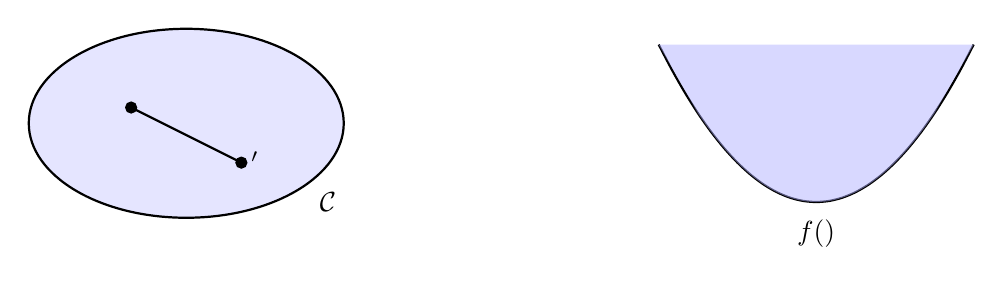
\begin{tikzpicture}
					\fill[blue!20, opacity=0.5] (-3,0) ellipse (2 and 1.2); 
					\draw[thick] (-3,0) ellipse (2 and 1.2);
					\filldraw[black] (-3.7,0.2) circle (2pt) node[left] {$\vw$};
					\filldraw[black] (-2.3,-0.5) circle (2pt) node[right] {$\vw'$};
					\draw[thick] (-3.7,0.2) -- (-2.3,-0.5);
					\node at (-1.2,-1.0) {$\mathcal{C}$};
					\begin{scope}[shift={(5,-1)}]
						\draw[thick, domain=-2:2, smooth, variable=\x] 
						plot ({\x}, {0.5*\x*\x});
						\fill[blue!30, opacity=0.5] 
						plot[domain=-1.5:1.5, smooth] ({\x}, {0.5*\x*\x}) -- 
						(2, {0.5*2*2}) -- 
						(-2, {0.5*2*2}) -- 
						cycle;
						\node at (0,-0.4) {$f(\weights)$};
					\end{scope}
				\end{tikzpicture}
				\vspace*{-8mm}
			\end{center}
			\caption{Gauche: Un ensemble convexe $\cluster \subseteq \mathbb{R}^{\dimlocalmodel}$. 
				Droite: Une \gls{function} convexe $f: \mathbb{R}^{\dimlocalmodel} \rightarrow \mathbb{R}$.
				\label{fig_convex_set_function_dict}}
		\end{figure}
	},
	first={convexe},
	text={convexe}
}

\newglossaryentry{linreg}{
	name={régression linéaire},
	description={La \index{régression linéaire} \gls{regression} linéaire vise à apprendre une fonction \gls{hypothesis} linéaire pour prédire une \gls{label} numérique à partir des \glspl{feature} numériques d’un \glspl{datapoint}. La qualité d’une fonction \gls{hypothesis} linéaire est mesurée par la moyenne de la \gls{sqerrloss} subie sur un ensemble de \glspl{labeled datapoint}, que nous appelons l'\gls{trainset}.},
	first={régression linéaire},
	text={régression linéaire}, plural={régressions linéaires}
}

\newglossaryentry{pseudoinverse}{
	name={pseudo-inverse},
	description={La \index{pseudo-inverse}pseudo-inverse de Moore–Penrose $\mA^{+}$ d’une matrice $\mA \in \mathbb{R}^{\samplesize \times \nrfeatures}$ généralise la notion d'\gls{inverse} \cite{GolubVanLoanBook}. La pseudo-inverse apparaît naturellement dans le cadre de la \gls{ridgeregression} appliquée à un \gls{dataset} avec des \glspl{label} arbitraires $\vy$ et une \gls{featuremtx} $\mX = \mA$ \cite[Ch.\ 3]{hastie01statisticallearning}. Les \gls{modelparams} appris par la \gls{ridgeregression} sont donnés par
		\[
		\widehat{\vw}^{(\regparam)}  = \big(\mA^T \mA + \regparam \mI \big)^{-1} \mA^\top \vy, \quad \regparam > 0.
		\]
		On peut alors définir la pseudo-inverse $\mA^+ \in \mathbb{R}^{\nrfeatures \times \samplesize}$ avec la limite \cite[Ch. 3]{benisrael2003generalized}
		\[
		\lim_{\regparam \to 0^+} \widehat{\vw}^{(\regparam)} = \mA^+ \vy.
		\]
		Voir aussi : \gls{inverse}, \gls{ridgeregression}, \gls{dataset}, \gls{label}, \gls{featuremtx}, \gls{modelparams}, \gls{ridgeregression}.
	},
	first={pseudo-inverse},
	text={pseudo-inverse}
}

\newglossaryentry{probability}{
	name={probabilité},
	description={On\index{probabilité} associe une valeur de probabilité, typiquement choisie dans l’intervalle $[0,1]$, à chaque événement pouvant se produire dans une expérience aléatoire \cite{KallenbergBook,BertsekasProb,BillingsleyProbMeasure,HalmosMeasure}.},
	first={probabilité},
	text={probabilité}
}

\newglossaryentry{euclidspace}{
	name={espace euclidien},
	description={L’\index{espace euclidien}espace euclidien $\mathbb{R}^{\featuredim}$ de dimension $\featuredim \in \mathbb{N}$ est constitué des vecteurs $\featurevec= \big(\feature_{1},\ldots,\feature_{\featurelen}\big)$, avec $\featuredim$ composantes réelles $\feature_{1},\ldots,\feature_{\featuredim} \in \mathbb{R}$. Un tel espace euclidien est muni d’une structure géométrique définie par le produit scalaire $\featurevec^{T} \featurevec' = \sum_{\featureidx=1}^{\featuredim} \feature_{\featureidx} \feature'_{\featureidx}$ entre deux vecteurs  $\featurevec,\featurevec' \in \mathbb{R}^{\featuredim}$ quelconques \cite{RudinBookPrinciplesMatheAnalysis}.},
	first={espace euclidien},
	text={espace euclidien}
}

\newglossaryentry{iid}{
	name={indépendantes et identiquement distribuées (i.i.d.)},
	description={Il\index{indépendantes et identiquement distribuées (i.i.d.)} peut être utile d’interpréter des \glspl{datapoint} $\datapoint^{(1)},\ldots,\datapoint^{(\samplesize)}$ comme des \glspl{realization} de \glspl{rv} i.i.d. suivant une \gls{probdist} commune. Si ces \glspl{rv} sont à valeurs continues, leur \gls{pdf} conjointe est $p\big(\datapoint^{(1)},\ldots,\datapoint^{(\samplesize)} \big) = \prod_{\sampleidx=1}^{\samplesize} p \big(\datapoint^{(\sampleidx)}\big)$, où $p(\datapoint)$ est la \gls{pdf} marginale commune des \glspl{rv} sous-jacentes (i.e., dont les \glspl{datapoint} sont les \glspl{realization}).},
	first={indépendantes et identiquement distribuées (i.i.d.)},
	text={{i.i.d.}}
}

\newglossaryentry{pdf}{name={fonction de densité de probabilité},
	description={La\index{fonction de densité de probabilité} fonction de densité de probabilité $p(\feature)$ 
		d’une \gls{rv} réelle $\feature \in \mathbb{R}$ est une représentation particulière de sa \gls{probdist}. 
		Si la fonction de densité de probabilité existe, elle peut être utilisée pour calculer la \gls{probability} que $\feature$ prenne une valeur 
		dans un ensemble (mesurable) $\mathcal{B} \subseteq \mathbb{R}$ avec $\prob{\feature \in \mathcal{B}} = \int_{\mathcal{B}} p(\feature') d \feature'$ \cite[Ch. 3]{BertsekasProb}. La fonction de densité de probabilité d’une \gls{rv} vectorielle $\featurevec \in \mathbb{R}^{\featuredim}$ (si elle existe) 
		permet de calculer la \gls{probability} que $\featurevec$ appartienne à une région (mesurable) $\mathcal{R}$ avec 
		$\prob{\featurevec \in \mathcal{R}} = \int_{\mathcal{R}} p(\featurevec') d \feature_{1}' \ldots d \feature_{\featuredim}' $ \cite[Ch. 3]{BertsekasProb}.},
	first={fonction de densité de probabilité},text={fonction de densité de probabilité}, plural={fonctions de densité de probabilite}}

%Texte non traduit après ce commentaire

\newglossaryentry{minimum}
{
	name=minimum,
	description={Given a set of real numbers, the minimum\index{minimum} is the smallest of those numbers.},
	first={minimum},text={minimum}
}

\newglossaryentry{boosting}
{name = {boosting}, 
	description={Boosting\index{boosting} is an iterative optimization method to learn an accurate 
		\gls{hypothesis} map (or strong learner) by sequentially combining less accurate 
		\gls{hypothesis} maps (referred to as weak learners) \cite[Ch. 10]{hastie01statisticallearning}.
		For example, weak learners are shallow \gls{decisiontree}s which are combined to 
		obtain a deep \gls{decisiontree}. Boosting can be understood as a generalization 
		of \gls{gdmethods} for \gls{erm} using parametric \gls{model}s and \gls{smooth} \gls{lossfunc}s 
		\cite{Friedman2001}. Just like \gls{gd} iteratively updates \gls{modelparams} to reduce the \gls{emprisk}, 
		boosting iteratively combines (e.g., by summation) \gls{hypothesis} maps to reduce the \gls{emprisk}. 
		A widely-used instance of the generic boosting idea is referred to as \gls{gradient} boosting, which 
		uses \gls{gradient}s of the \gls{lossfunc} for combining the weak learners \cite{Friedman2001}. 
		\begin{figure}
			\begin{center}
				\begin{tikzpicture}[scale=1.2]
					% Axes
					\draw[->] (-0.5,0) -- (5.5,0) node[right] {$\hypothesis$};
					\draw[->] (0,-0.5) -- (0,4.5) node[above] {$\lossfunc{\vz}{\hypothesis}$};
					%					% Loss curve
					\draw[thick,domain=0.2:5,smooth,variable=\x,blue!60] plot ({\x},{(4 - 1.3*\x + 0.15*\x*\x)});
					%	\node[blue] at (4.5,2.2) {\gls{loss}};
					%					% Points on the curve
					\foreach \x/\label in {0.7/$\hypothesis^{(0)}$, 1.5/$\hypothesis^{(1)}$, 2.3/$\hypothesis^{(2)}$, 3.0/$\hypothesis^{(3)}$} {
						\draw[dashed, gray] (\x, 0) -- (\x, {4 - 1.3*\x + 0.15*\x*\x}); % helper line
						\filldraw[black] (\x, {4 - 1.3*\x + 0.15*\x*\x}) circle (2pt);   % point
						\node[below] at (\x, -0.1) {\label};                             % label
					}
					%					% Arrows for descent
					%					\foreach \x/\xnext in {0.7/1.5, 1.5/2.3, 2.3/3.0} {
						%						\draw[->,red,thick] (\x,{(4 - 1.3*\x + 0.15*\x*\x)}) -- (\xnext,{(4 - 1.3*\xnext + 0.15*\xnext*\xnext)});
						%					}
					%					% Gradient label
					%					\node[red] at (1.8,3.6) {Update direction $\approx -\nabla \text{Loss}$};
				\end{tikzpicture}
			\end{center} 
			\caption{Boosting methods construct a sequence of \gls{hypothesis} maps $\hypothesis^{(0)},\hypothesis^{(1)},\ldots$ 
				that are increasingly strong learners (i.e., incurring a smaller \gls{loss}).}
		\end{figure} 
		\\ See also: \gls{gradstep}, \gls{gdmethods}
	}, 
	first={boosting}, 
	text={boosting}} 


\newglossaryentry{maximum}
{name=maximum,
     description={The maximum\index{maximum} of a set $\mathcal{A} \subseteq \mathbb{R}$ 
     	of real numbers is the greatest element in that set, if such an element exists. A set $\mathcal{A}$ 
     	has a maximum if it is bounded above and attains its \gls{supremum} \cite[Sec.~1.4]{RudinBookPrinciplesMatheAnalysis}.},
 first={maximum},text={maximum}
}

\newglossaryentry{supremum}
{name=borne supérieure,
	description={The supremum\index{borne supérieure} of a set of real numbers is 
		the smallest number that is greater than or equal to every element in the set. More formally, a 
		real number $a$ is the supremum of a set $\mathcal{A} \subseteq \mathbb{R}$ if: 1) $a$ 
		is an upper bound of $\mathcal{A}$; and 2) no number smaller than $a$ is an upper bound of $\mathcal{A}$. 
		Every non-empty set of real numbers that is bounded above has a supremum, even if it does 
		not contain its supremum as an element \cite[Sec.~1.4]{RudinBookPrinciplesMatheAnalysis}.},
	first={supremum (or least upper bound)},text={supremum}
}

\newglossaryentry{discrepancy}
{name=discrepancy,
	description={
		Consider\index{discrepancy} an \gls{fl} application with \gls{netdata} 
		represented by an \gls{empgraph}. \gls{fl} methods use a discrepancy measure 
		to compare \gls{hypothesis} maps from \gls{localmodel}s at nodes $\nodeidx,\nodeidx'$ 
		connected by an edge in the \gls{empgraph}.},
	first={discrepancy},text={discrepancy}
}

\newglossaryentry{FedGD}
{name={FedGD},
	description={An\index{FedGD} \gls{fl} \gls{distributedalgorithm} that 
		can be implemented as message passing across an \gls{empgraph}. 
		\\ 
		See also: \gls{fl}, \gls{algorithm}, \gls{gradstep}, \gls{gdmethods}.},
	first={FedGD},text={FedGD}
} 

\newglossaryentry{FedSGD}
{name={FedSGD},
	description={An\index{FedSGD} \gls{fl} \gls{distributedalgorithm} that 
		can be implemented as message passing across an \gls{empgraph}. 
		\\ 
		See also: \gls{fl}, \gls{algorithm}, \gls{gradstep}, \gls{gdmethods}, \gls{stochGD}.},
	first={FedSGD},text={FedSGD}
} 

\newglossaryentry{hfl}
{name={horizontal federated learning (HFL)},description=
	{HFL\index{horizontal federated learning (HFL)} uses \gls{localdataset}s constituted by different
		\gls{datapoint}s but uses the same \gls{feature}s to characterize them \cite{HFLChapter2020}.
		For example, weather forecasting uses a network of spatially distributed
		weather (observation) stations. Each weather station measures the
		same quantities, such as daily temperature, air pressure, and precipitation.
		However, different weather stations measure the characteristics or
		\gls{feature}s of different spatiotemporal regions. Each spatiotemporal region 
		represents an individual \gls{datapoint}, each characterized by the same \gls{feature}s 
		(e.g., daily temperature or air pressure).\\
		See also: \gls{fl}, \gls{vfl}, \gls{cfl}. },
	first={HFL},text={HFL}
} 

\newglossaryentry{dimred}
{name={réduction de dimension},
	description={Dimensionality reduction\index{réduction de dimension} methods 
		map (typically many) raw \gls{feature}s to a (relatively small) set of 
		new \gls{feature}s. These methods can be used to visualize \gls{datapoint}s 
		by learning two \gls{feature}s that can be used as the coordinates of a 
		depiction in a \gls{scatterplot}.}, first={réduction de dimension},text={réduction de dimension}
} 


\newglossaryentry{featlearn}
{name={feature learning},
	description={Consider an \gls{ml} application with \gls{datapoint}s characterized by 
		raw \gls{feature}s $\featurevec \in \featurespace$. \Gls{feature} learning\index{feature learning} 
		refers to the task of learning a map 
		$$\featuremapvec: \featurespace \rightarrow \featurespace': \featurevec \mapsto \featurevec',$$ 
		that reads in raw \gls{feature}s $\featurevec \in \featurespace$ of a \gls{datapoint} and delivers new 
		\gls{feature}s $\featurevec' \in \featurespace'$ from a new \gls{featurespace} $\featurespace'$. 
		Different \gls{feature} learning methods are obtained for different design 
		choices of $\featurespace,\featurespace'$, for a \gls{hypospace} $\hypospace$ 
		of potential maps $\featuremapvec$, and for a quantitative measure of the usefulness of 
		a specific $\featuremapvec \in \hypospace$. For example, \gls{pca} 
		uses $\featurespace \defeq \mathbb{R}^{\dimlocalmodel}$, $\featurespace' \defeq \mathbb{R}^{\dimlocalmodel'}$ 
		with $\dimlocalmodel' < \dimlocalmodel$, and a \gls{hypospace} 
		$$\hypospace\defeq \big\{ \featuremapvec: \mathbb{R}^{\dimlocalmodel}
		\!\rightarrow\! \mathbb{R}^{\dimlocalmodel'}\!:\!\featurevec'\!\defeq\!\mF \featurevec \mbox{ with some } \mF \!\in\! \mathbb{R}^{\dimlocalmodel' \times \dimlocalmodel} \big\}.$$ \Gls{pca} measures the usefulness of a specific map $\featuremapvec(\featurevec)= \mF \featurevec$ 
	by the \gls{minimum} linear reconstruction error incurred on a \gls{dataset}, 
$$ \min_{\mG \in \mathbb{R}^{\dimlocalmodel \times \dimlocalmodel'}} \sum_{\sampleidx=1}^{\samplesize} \normgeneric{\mG \mF \featurevec^{(\sampleidx)} - \featurevec^{(\sampleidx)}}{2}^{2}.$$ }, 
	first={feature learning},text={feature learning}
} 

\newglossaryentry{autoencoder}
{name={autoencoder},
	description={An autoencoder\index{autoencoder} is an \gls{ml} method that simultaneously learns an encoder map 
		$\hypothesis(\cdot) \in \hypospace$ and a decoder map $\hypothesis^{*}(\cdot) \in \hypospace^{*}$. 
		It is an instance of \gls{erm} using a \gls{loss} computed from the reconstruction error 
		$\featurevec - \hypothesis^{*}\big(  \hypothesis \big( \featurevec \big) \big)$.},
	first={autoencoder},text={autoencoder}
} 

\newglossaryentry{vfl}
{name={vertical federated learning (vertical FL)},description=
	{Vertical \gls{fl}\index{vertical federated learning (vertical FL)} uses \gls{localdataset}s that are constituted 
	 by the same \gls{datapoint}s but characterizing them with different \gls{feature}s \cite{VFLChapter}. 
     For example, different healthcare providers might all contain information 
     about the same population of patients. However, different healthcare providers 
     collect different measurements (e.g., blood values, electrocardiography, lung X-ray) 
     for the same patients.},
	first={vertical federated learning (vertical FL)},text={vertical FL}
} 

\newglossaryentry{interpretability}
{name={interpretability},description=
		{An \gls{ml} method is interpretable\index{interpretability} for a specific user if 
			they can well anticipate the \gls{prediction}s delivered by the method. 
			The notion of interpretability can be made precise using quantitative 
			measures of the uncertainty about the \gls{prediction}s \cite{JunXML2020}.},
		first={interpretability},text={interpretability}
}

\newglossaryentry{explainability}
{name={explainability},description=
		{We\index{explainability} define the (subjective) explainability of an \gls{ml} method 
			as the level of simulatability \cite{Colin:2022aa} of the \gls{prediction}s 
			delivered by an \gls{ml} system to a human user. Quantitative measures for the 
			(subjective) explainability of a trained \gls{model} can be constructed by 
			comparing its \gls{prediction}s with the \gls{prediction}s provided by a user 
			on a \gls{testset} \cite{Zhang:2024aa,Colin:2022aa}. Alternatively, we can use 
			\gls{probmodel}s for \gls{data} and measure the explainability of a trained \gls{ml} 
			\gls{model} via the conditional (differential) entropy of its \gls{prediction}s, given the user \gls{prediction}s \cite{JunXML2020,Chen2018}. 
		},
		first={explainability},text={explainability}
	}
	
\newglossaryentry{lime}
{name={Local Interpretable Model-agnostic Explanations (LIME)},description={
		Consider\index{Local Interpretable Model-agnostic Explanations (LIME)} 
		a trained \gls{model} (or learnt \gls{hypothesis}) $\widehat{\hypothesis} \in \hypospace$, 
		which maps the \gls{featurevec} of a \gls{datapoint} to the \gls{prediction} $\widehat{\truelabel}= \widehat{\hypothesis}$. 
		Local Interpretable Model-agnostic Explanations (LIME) is a technique for explaining 
		the behaviour of $\widehat{\hypothesis}$, locally around a \gls{datapoint} with \gls{featurevec} $\featurevec^{(0)}$ \cite{Ribeiro2016}. 
		The explanation is given in the form of a local approximation $g \in \hypospace'$ of $\widehat{\hypothesis}$ (see Fig.\ \ref{fig_lime}). 
		This approximation can be obtained by an instance of \gls{erm} with carefully designed 
		\gls{trainset}. In particular, the \gls{trainset} consists of \gls{datapoint}s with 
		\gls{featurevec} $\featurevec$ close to $\featurevec^{(0)}$ and the (pseudo-)label $\widehat{\hypothesis}(\featurevec)$. 
		Note that we can use a different \gls{model} $\hypospace'$ for the approximation than 
		the original \gls{model} $\hypospace$. For example, we can use a \gls{decisiontree} 
		to approximate (locally) a \gls{deepnet}. Another widely-used choice for $\hypospace'$ is 
		the \gls{linmodel}. 
		\begin{figure}[htbp]
		\begin{center}
		\begin{tikzpicture}
			\begin{axis}[
				axis lines=middle,
				xlabel={$\featurevec$},
				ylabel={$\truelabel$},
				xtick=\empty,
				ytick=\empty,
				xmin=0, xmax=6,
				ymin=0, ymax=6,
				domain=0:6,
				samples=100,
				width=10cm,
				height=6cm,
				clip=false
			]
			  % Non-linear model h(x)
  			\addplot[blue, thick, domain=0:6] {2 + sin(deg(x))} node[pos=0.85, above right,yshift=3pt] {$\widehat{\hypothesis}(\featurevec)$};
			 % Feature value x0
  			\addplot[dashed, gray] coordinates {(3,0) (3,6)};
			% Piecewise constant local approximation g(x)
  			\addplot[red, thick, domain=2.5:3.5] {2 + sin(deg(3))} node[pos=0.9, above] {$g(\featurevec)$};
			% Optional: mark the point of approximation
  			\addplot[mark=*] coordinates {(3, {2 + sin(deg(3))})};
			\node at (axis cs:3,-0.3) {$\featurevec^{(0)}$};
			\end{axis}
		  \end{tikzpicture}
		\end{center}
		\caption{To explain a trained \gls{model} $\widehat{\hypothesis} \in \hypospace$, around a 
		given \gls{featurevec} $\featurevec^{(0)}$, we can use a local approximation $g \in \hypospace'$. }
		\end{figure}\label{fig_lime}},
	first={LIME},text={LIME}
}
	
	
\newglossaryentry{gradstep}{name={gradient step},description={Given a \gls{differentiable} 
		real-valued function $f(\cdot): \mathbb{R}^{\nrfeatures} \rightarrow \mathbb{R}$ 
		 and a vector $\weights \in \mathbb{R}^{\nrfeatures}$, the \gls{gradient} step\index{gradient step} 
		 updates $\weights$ by adding the scaled negative \gls{gradient} $\nabla f(\weights)$ to obtain 
		 the new vector (see Figure \ref{fig_basic_GD_step_single_dict})
		 \begin{equation}
		 \label{equ_def_gd_basic_dict} 
		\widehat{\weights}  \defeq \weights - \lrate \nabla f(\weights).
		\end{equation} 
		Mathematically, the \gls{gradient} step is a (typically non-linear) operator $\mathcal{T}^{(f,\lrate)}$ 
		that is parametrized by the function $f$ and the \gls{stepsize} $\lrate$. 
		\begin{figure}[H]
			\begin{center}
				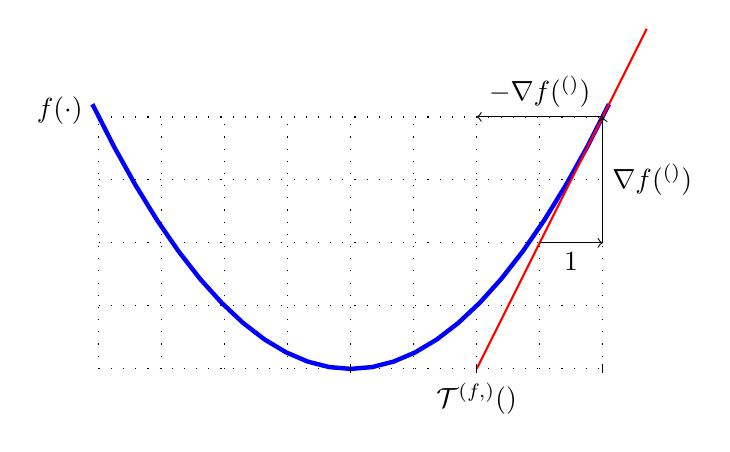
\begin{tikzpicture}[scale=0.8]
					\draw[loosely dotted] (-4,0) grid (4,4);
					\draw[blue, ultra thick, domain=-4.1:4.1] plot (\x,  {(1/4)*\x*\x});
					\draw[red, thick, domain=2:4.7] plot (\x,  {2*\x - 4});
					\draw[<-] (4,4) -- node[right] {$\nabla f(\weights^{(\itercntr)})$} (4,2);
					\draw[->] (4,4) -- node[above] {$-\lrate \nabla f(\weights^{(\itercntr)})$} (2,4);
					\draw[<-] (4,2) -- node[below] {$1$} (3,2) ;
					%\draw[->] (-4.25,0) -- (4.25,0) node[right] {$a$};
					\node[left] at (-4.1, 4.1) {$f(\cdot)$}; 
					\draw[shift={(0,0)}] (0pt,2pt) -- (0pt,-2pt) node[below] {$\overline{\weights}$};
					\draw[shift={(4,0)}] (0pt,2pt) -- (0pt,-2pt) node[below] {$\weights$};
					\draw[shift={(2,0)}] (0pt,2pt) -- (0pt,-2pt) node[below] {$\mathcal{T}^{(f,\lrate)}(\weights)$};
				\end{tikzpicture}
			\end{center}
			\caption{The basic \gls{gradient} step \eqref{equ_def_gd_basic_dict} maps a given vector $\weights$ 
			to the updated vector $\weights'$. It defines an operator 
			$\mathcal{T}^{(f,\lrate)}(\cdot): \mathbb{R}^{\nrfeatures} \rightarrow \mathbb{R}^{\nrfeatures}:
			 \weights \mapsto \widehat{\weights}$.}
			\label{fig_basic_GD_step_single_dict}
		\end{figure}
		Note that the \gls{gradient} step \eqref{equ_def_gd_basic_dict} optimizes locally - 
		in a \gls{neighborhood} whose size is determined by the \gls{stepsize} $\lrate$ - a linear approximation 
		to the function $f(\cdot)$. A natural \gls{generalization} of \eqref{equ_def_gd_basic_dict} is to locally 
		optimize the function itself - instead of its linear approximation - such that
		\begin{align} 
		\label{equ_approx_gd_step_dict}
		\widehat{\weights} = \argmin_{\weights' \in \mathbb{R}^{\dimlocalmodel}} f(\weights')\!+\!(1/\lrate)\normgeneric{\weights-\weights'}{2}^2. 
		\end{align}
		We intentionally use the same symbol $\lrate$ for the parameter in \eqref{equ_approx_gd_step_dict} 
		as we used for the \gls{stepsize} in \eqref{equ_def_gd_basic_dict}. The larger the $\lrate$ we choose in 
		\eqref{equ_approx_gd_step_dict}, the more progress the update will make towards reducing the 
		function value $f(\widehat{\weights})$. Note that, much like the \gls{gradient} step \eqref{equ_def_gd_basic_dict}, 
		also the update \eqref{equ_approx_gd_step_dict} defines a (typically non-linear) operator 
		that is parametrized by the function $f(\cdot)$ and the parameter $\lrate$. For a \gls{convex} function 
		$f(\cdot)$, this operator is known as the \gls{proxop} of $f(\cdot)$ \cite{ProximalMethods}. 
		},first={gradient step},text={gradient step}}
	

\newglossaryentry{proxop}{name={proximal operator},description={Given\index{proximal operator} a \gls{convex} 
		function $f(\weights')$, we define its proximal operator as \cite{ProximalMethods,Bauschke:2017} 
		$$\proximityop{f(\cdot)}{\weights}{\rho}\defeq \argmin_{\weights' \in \mathbb{R}^{\dimlocalmodel}} \bigg[ f(\weights')\!+\!(\rho/2) \normgeneric{\weights- \weights'}{2}^{2}\bigg] \mbox{ with } \rho > 0. $$ 
		As illustrated in Figure \ref{fig_proxoperator_opt_dict}, evaluating the proximal operator 
		amounts to minimizing a penalized variant of $f(\weights')$. The penalty term is the 
		scaled squared Euclidean distance to a given vector $\weights$ (which is the input to the proximal operator). 
		%\Gls{convex} functions for which the proximal operator can be computed efficiently 
		%is sometimes referred to as \emph{proximable} or \emph{simple} \cite{Condat2013}. 
		The proximal operator can be interpreted as a \gls{generalization} of the \gls{gradstep}, which is defined 
		for a \gls{smooth} \gls{convex} function $f(\weights')$. Indeed, taking a 
		\gls{gradstep} with \gls{stepsize} $\lrate$ at the current vector $\weights$ 
		is the same as applying the \gls{proxop} of the function $\tilde{f}(\weights')= \big( \nabla f(\weights)\big)^{T} (\weights'-\weights)$ 
		and using $\rho=1/\lrate$.
			\begin{figure}[H]
			\begin{center}
				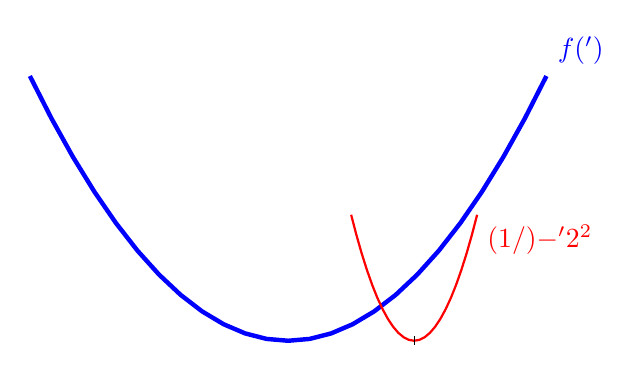
\begin{tikzpicture}[scale=0.8]
					% Original quadratic function
					\draw[blue, ultra thick, domain=-4.1:4.1] plot (\x, {(1/4)*\x*\x}) node[above right] {$f(\weights')$};		
					% Quadratic function with larger curvature, centered at w = 2
					\draw[red, thick, domain=1:3] plot (\x, {2*(\x - 2)*(\x - 2)}) node[below right] {$(1/\lrate)\normgeneric{\weights-\weights'}{2}^{2}$};
					% Axes
					% Minimum point of second curve
					\draw[shift={(2,0)}] (0pt,2pt) -- (0pt,-2pt) node[below] {$\weights$};
					%\node at (2,0.5) [anchor=north] {$\weights$};
				\end{tikzpicture}
			\end{center}
			\caption{A generalized \gls{gradstep} updates a vector $\weights$ by minimizing a penalized version 
				of the function $f(\cdot)$. The penalty term is the scaled squared Euclidean distance between the optimization 
				variable $\weights'$ and the given vector $\weights$.	\label{fig_proxoperator_opt_dict}}
		\end{figure}
		},first={proximal operator},text={proximal operator}}

\newglossaryentry{proximable}{name={proximable},description={A\index{proximable} 
		\gls{convex} function for which the \gls{proxop} can be computed efficiently is 
		sometimes referred to as proximable or simple \cite{Condat2013}.},first={proximable},text={proximable}}


\newglossaryentry{connected}{name ={connected graph}, description={An\index{connected graph} 
		undirected \gls{graph} $\graph=\pair{\nodes}{\edges}$ is connected\index{connected graph} if every 
		non-empty subset $\nodes' \subset \nodes$ has at least one edge connecting it to $\nodes \setminus \nodes'$.}, 
		first={connected graph},text={connected graph}}


\newglossaryentry{statasp}{name ={statistical aspects}, description={By statistical aspects\index{statistical aspects} 
		of an \gls{ml} method, we refer to (properties of) the \gls{probdist} of its output 
		under a \gls{probmodel} for the \gls{data} fed into the method.},first={statistical aspects},text={statistical aspects}}

\newglossaryentry{compasp}{name ={computational aspects}, description={By computational 
		aspects\index{computational aspects} of an \gls{ml} method, we mainly refer to the computational 
		resources required for its implementation. For example, if an \gls{ml} method uses iterative 
		optimization techniques to solve \gls{erm}, then its computational aspects include: 1) how 
		many arithmetic operations are needed to implement a single iteration (\gls{gradstep}); 
		and 2) how many iterations are needed to obtain useful \gls{modelparams}. One important 
		example of an iterative optimization technique is \gls{gd}.}, first={computational aspects},text={computational aspects}}

\newglossaryentry{zerooneloss}{name={$\bf 0/1$ loss},
	description={The $0/1$ \gls{loss}\index{$0/1$ loss} $\lossfunczo{\pair{\featurevec}{\truelabel}}{\hypothesis}$ 
		measures the quality of a \gls{classifier} $\hypothesis(\featurevec)$ that delivers a 
		\gls{prediction} $\predictedlabel$ (e.g., via thresholding \eqref{equ_def_threshold_bin_classifier_dict}) 
		for the \gls{label} $\truelabel$ of a \gls{datapoint} with \gls{feature}s $\featurevec$. It is equal to $0$ if 
		the \gls{prediction} is correct, i.e., 
	$\lossfunczo{\pair{\featurevec}{\truelabel}}{\hypothesis}=0$ when $\predictedlabel=\truelabel$. It is 
	equal to $1$ if the \gls{prediction} is wrong, i.e., $\lossfunczo{\pair{\featurevec}{\truelabel}}{\hypothesis}=1$ 
	when $\predictedlabel\neq\truelabel$.},
	sort=zerooneloss, 
    first={$0/1$ loss},text={$0/1$ loss}}
	
\newglossaryentry{underfitting}{name={sous-apprentissage},description={Consider\index{sous-apprentissage} 
		an \gls{ml} method that uses \gls{erm} to learn a \gls{hypothesis} with the \gls{minimum} \gls{emprisk} 
		on a given \gls{trainset}. Such a method is underfitting the \gls{trainset} if it is 
		not able to learn a \gls{hypothesis} with a sufficiently small \gls{emprisk} on the \gls{trainset}. 
		If a method is underfitting, it will typically also not be able to learn a \gls{hypothesis} with 
		a small \gls{risk}.},first={sous-apprentissage},text={sous-apprentissage}}

\newglossaryentry{overfitting}{name={surapprentissage},description={Consider\index{surapprentissage} an 
		\gls{ml} method that uses \gls{erm} to learn a \gls{hypothesis} with the \gls{minimum} \gls{emprisk} on 
		a given \gls{trainset}. Such a method is overfitting the \gls{trainset} if it learns 
		a \gls{hypothesis} with a small \gls{emprisk} on the \gls{trainset} but a significantly larger \gls{loss} outside the \gls{trainset}.},first={surapprentissage},text={surapprentissage}}

\newglossaryentry{gdpr}{name={Règlement général sur la protection des données (RGPD)},description={
			The\index{règlement général sur la protection des données (RGPD)} GDPR
			was enacted by the European Union (EU), effective from May 25, 2018 \cite{GDPR2016}. 
			It safeguards the privacy and \gls{data} rights of individuals in the EU. 
			The GDPR has significant implications for how \gls{data} is collected, stored, and used in \gls{ml}  
			applications. Key provisions include the following:
			\begin{itemize}
				\item \Gls{dataminprinc}: \gls{ml} systems should only use the necessary amount of personal 
				\gls{data} for their purpose.
				\item \Gls{transparency} and \gls{explainability}: \gls{ml} systems should enable their users to 
				understand how the systems make decisions that impact the users.
				\item \Gls{data} subject rights: Users should get an opportunity to access, rectify, and delete their personal \gls{data}, as well as to object to automated decision-making and profiling.
				\item Accountability: Organizations must ensure robust \gls{data} security and demonstrate 
				compliance through documentation and regular audits.
			\end{itemize}
			}, 
	first={règlement général sur la protection des données (RGPD)},text={RGPD}}



\newglossaryentry{GaussProc}
{name={Gaussian process (GP)},
	description={A \index{Gaussian Process (GP)}GP is a collection of \gls{rv}s 
		$\{f(\featurevec)\}_{\featurevec \in \featurespace}$ indexed by input values $\featurevec$ 
		from some input space $\featurespace$, such that for any finite subset 
		$\featurevec^{(1)}, \ldots, \featurevec^{(\samplesize)} \in \featurespace$, 
		the corresponding \gls{rv}s $f(\featurevec^{(1)}, \ldots, \featurevec^{(\samplesize)}$ have a joint 
		multivariate Gaussian distribution:
		\[
		\left( f(\featurevec^{(1)}, \ldots, \featurevec^{(\samplesize)} \right) \sim \mathcal{N}(\boldsymbol{\mu}, \mathbf{K}).
		\]
		For a fixed input space $\featurespace$, a GP is fully specified (or parametrized) by 
		\begin{itemize}
			\item a \gls{mean} function $\mu(\featurevec) = \expect\{ f(\featurevec)\}$,
			\item and a covariance function $\kernelmap{\featurevec}{\featurevec'}= \expect\{ \big(f(\featurevec)-\mu(\featurevec)\big) \big(f(\featurevec')-\mu(\featurevec')\big) \big\}$.
		\end{itemize}
		\textbf{Example.} We can interpret the temperature distribution across Finland (at a specific 
		point in time) as the \gls{realization} of a GP $f(\featurevec)$, where each input $\featurevec = (\text{lat}, \text{lon})$ 
		denotes a geographic location. Temperature observations from \gls{fmi} weather stations provide 
		samples of $f(\featurevec)$ at specific locations (see Fig.\ \ref{fig_gp_FMI}). A GP allows to 
		predict the temperature nearby \gls{fmi} weather stations and to quantify the uncertainty 
		of these predictions. 
		\begin{figure}[H]
			\begin{center}
				\begin{tikzpicture}
					\begin{axis}[
						axis equal,
						hide axis,
						scale=1.2,
						xmin=17, xmax=32,
						ymin=55, ymax=71,
						%	width=15cm,
						%	height=20cm,
						clip=true
						]
						% --- Finland border (polyline) ---
						\addplot[
						color=black,
						thick
						] table [x=lon, y=lat, col sep=comma] {assets/finland_border.csv};
						% --- FMI sample stations ---
						\addplot[
						only marks,
						mark=*,
						mark options={fill=blue},
						color=black
						] table [x=lon, y=lat, col sep=comma] {assets/fmi_stations_subset.csv};
						% Draw manual axes
						\draw[->, thick] (axis cs:19,59) -- (axis cs:25.5,59) node[anchor=west] {lon};
						\draw[->, thick] (axis cs:19,59) -- (axis cs:19,65.5) node[anchor=south] {lat};
					\end{axis}
				\end{tikzpicture}
				\vspace*{-15mm}
			\end{center}
			\caption{We can interpret the temperature distribution over Finland as a \gls{realization} 
				of a GP indexed by geographic coordinates and sampled at \gls{fmi} weather stations (indicated by 
				blue dots). \label{fig_gp_FMI}}
	\end{figure}}, 
	first = {Gaussian process}, 
	text = {GP}
}

\newglossaryentry{trustAI}
{name={trustworthy artificial intelligence (trustworthy AI)},
	description={Besides the \gls{compasp} and \gls{statasp}, a third main 
		design aspect of \gls{ml} methods is their trustworthiness\index{trustworthy AI} 
		\cite{pfau2024engineeringtrustworthyaideveloper}. 
		The EU has put forward seven key requirements (KRs) for trustworthy 
		\gls{ai} (that typically build on \gls{ml} methods)
		\cite{ALTAIEU}: 
		\begin{enumerate}[label=\arabic*)]
			\item KR1 - Human agency and oversight;
			\item KR2 - Technical robustness and safety;
			\item KR3 - Privacy and data governance;
			\item KR4 - Transparency;
			\item KR5 - Diversity, non-discrimination and fairness; 
			\item KR6 - Societal and environmental well-being;
			\item KR7 - Accountability. 
		\end{enumerate}
	},
	first={trustworthy artificial intelligence (trustworthy AI)},
	text={trustworthy AI}
}

\newglossaryentry{robustness}
{name=robustness,
	description={TBD},
	first={robustness},text={robustness}
}

\newglossaryentry{sqerrloss}{name={squared error loss},description={The squared 
		error\index{squared error loss} \gls{loss} measures the \gls{prediction} error of a 
		\gls{hypothesis} $\hypothesis$ when predicting a numeric \gls{label} $\truelabel \in \mathbb{R}$ 
		from the \gls{feature}s $\featurevec$ of a \gls{datapoint}. It is 
	defined as 
\begin{equation} 
	\nonumber
%	\label{equ_squared_loss_gls}
	\lossfunc{(\featurevec,\truelabel)}{\hypothesis} \defeq \big(\truelabel - \underbrace{\hypothesis(\featurevec)}_{=\predictedlabel} \big)^{2}. 
\end{equation} 
},first={squared error loss},text={squared error loss}}


 \newglossaryentry{projection}{name={projection}, 
       description={Consider\index{projection} a subset $\paramspace \subseteq \mathbb{R}^{\dimlocalmodel}$ of 
	   the $\dimlocalmodel$-dimensional \gls{euclidspace}. We define the projection $\projection{\paramspace}{\weights}$
	   of a vector $\weights \in \mathbb{R}^{\dimlocalmodel}$ onto $\paramspace$ as
		\begin{equation} 
   	    \label{equ_def_proj_generic_dict}
  	     \projection{\paramspace}{\weights} = \argmin_{\weights' \in \paramspace} \normgeneric{\weights - \weights'}{2}. 
         \end{equation}
		 In other words, $\projection{\paramspace}{\weights}$ is the vector in $\paramspace$ which is closest to $\weights$. 
		 The projection is only well-defined for subsets $\paramspace$ for which the above \gls{minimum} exists \cite{BoydConvexBook}.},
		 first={projection},text={projection}}


\newglossaryentry{projgd}{name={projected gradient descent (projected GD)},
description={Consider an \gls{erm}-based method that uses a parametrized \gls{model} with  
\gls{paramspace} $\paramspace \subseteq \mathbb{R}^{\dimlocalmodel}$. Even if 
the \gls{objfunc} of \gls{erm} is \gls{smooth}, we cannot use basic \gls{gd}, as 
it does not take into account contraints on the optimization variable (i.e., the \gls{modelparams}). 
Projected\index{projected gradient descent (projected GD)} \gls{gd} 
extends basic \gls{gd} to handle constraints on the optimization variable (i.e., the \gls{modelparams}). 
A single iteration of projected \gls{gd} consists of first taking a \gls{gradstep} 
and then projecting the result back onto the \gls{paramspace}.
\begin{figure}[H]
	\begin{center}
		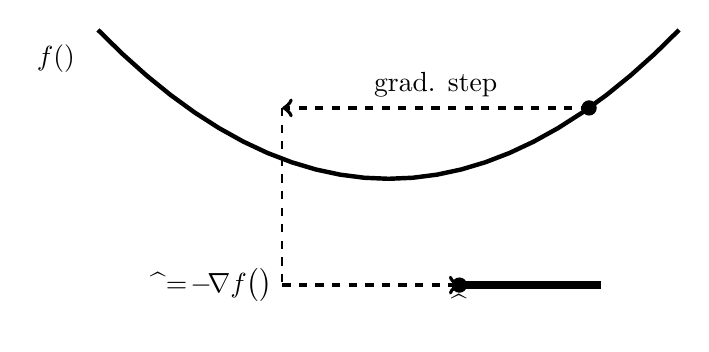
\begin{tikzpicture}[scale=0.9]
			\node [right] at (-5.1,1.7) {$f(\weights)$} ;
			\draw[ultra thick, domain=-4.1:4.1] plot (\x,  {(1/8)*\x*\x});
		%	\draw[dashed, thick, domain=1:3.6] plot (\x,  {\x - 1}) node[right] {$ f\big(\weights^{(\itercntr)}\big)\!+\!\big(\weights\!-\!\weights^{(\itercntr)}\big)^{T} \nabla f\big(\weights^{(\itercntr)}\big)$};
			\draw [fill] (2.83,1) circle [radius=0.1] node[right] {$\weights$};
			\draw[line width =0.5mm,dashed,->] (2.83,1) -- node[midway,above] {grad. step} (-1.5,1);
			\draw[line width =0.2mm,dashed] (-1.5,1) --(-1.5,-1.5)  node [below, left]{$\widehat{\weights}=\weights\!-\!\lrate \nabla f\big(\weights\big)$} ;
			\draw[line width =0.5mm,dashed,->] (-1.5,-1.5)  -- node[midway,above] {} (1,-1.5) ; 
			\draw [fill] (1,-1.5) circle [radius=0.1] node[below] {$\projection{\paramspace}{\widehat{\weights}}$};
			\draw[line width=1mm] (1,-1.5) -- (3,-1.5) node[midway, above] {$\paramspace$};
		\end{tikzpicture}
		\vspace*{-5mm}
	\end{center}
	\caption{Projected \gls{gd} augments a basic \gls{gradstep} with a \gls{projection} back 
	onto the constraint set $\paramspace$.}
	\label{fig_projected_GD_dict}
\end{figure}},first={projected gradient descent (projected GD)},text={projected GD}}

\newglossaryentry{diffpriv}
{name=differential privacy (DP),
  description={
  	Consider\index{differential privacy (DP)} some \gls{ml} method $\algomap$ that reads in a \gls{dataset} (e.g., the \gls{trainset} 
  	used for \gls{erm}) and delivers some output $\algomap(\dataset)$. The output 
  	could be either the learned \gls{modelparams} or the \gls{prediction}s for specific \gls{datapoint}s. 
  	DP is a precise measure of \gls{privleakage} incurred by revealing the 
  	output. Roughly speaking, an \gls{ml} method is differentially private if the \gls{probdist} 
  	of the output $\algomap(\dataset)$ does not change too much if the \gls{sensattr} 
  	of one \gls{datapoint} in the \gls{trainset} is changed. Note that DP 
  	builds on a \gls{probmodel} for an \gls{ml} method, i.e., we interpret its output $\algomap(\dataset)$ 
  	as the \gls{realization} of an \gls{rv}. The randomness in the output can be ensured 
  	by intentionally adding the \gls{realization} of an auxiliary \gls{rv} (noise) to 
  	the output of the \gls{ml} method.}, 
	first = {DP}, text={DP} 
}

\newglossaryentry{stability}
{name={stability},
	description={
		Stability\index{stability} is a desirable property of a \gls{ml} method $\algomap$ that maps a 
		\gls{dataset} $\dataset$ (e.g., a \gls{trainset}) to an output $\algomap(\dataset)$, such as learned 
		\gls{modelparams} or the \gls{prediction} for a specific \gls{datapoint}. Intuitively, $\algomap$ is 
		stable if small changes in the input \gls{dataset} $\dataset$ lead to small changes in the 
		output $\algomap(\dataset)$. Several formal notions of stability exist that enable bounds 
		on the \gls{generalization} error or \gls{risk} of the method; see \cite[Ch.~13]{ShalevMLBook}.
		To build intuition, consider the three datasets depicted in Fig.~\ref{fig_three_data_stability}, each 
		of which is equally likely under the same \gls{data}-generating \gls{probdist}. Since the 
		optimal \gls{modelparams} are determined by this underlying \gls{probdist}, an accurate 
		\gls{ml} method $\algomap$ should return the same (or very similar) output $\algomap(\dataset)$ 
		for all three \gls{dataset}. In other words, any useful $\algomap$ must be robust to 
		variability in sample \gls{realization}s from the same \gls{probdist}, i.e., it must be stable. 
		\begin{figure}[htbp]
			\centering
			\begin{tikzpicture}
				\begin{axis}[
				%title={Stem Plots of 3 Datasets},
				    axis lines=none,
					xlabel={$\sampleidx$},
					ylabel={},
					legend pos=north west,
					ymin=0, ymax=10,
					xtick={1,2,3,4,5},
				%	ymajorgrids=true,
					grid style=dashed,
					every axis plot/.append style={very thick}
					]
					% Dataset 1
					\addplot+[only marks,mark=*] coordinates {
						(1,2) (2,4) (3,3) (4,5) (5,7)
					};
				%	\addlegendentry{$\dataset^{(*)}$}
					% Dataset 2
					\addplot+[only marks,mark=square*] coordinates {
						(1,3) (2,2) (3,6) (4,4) (5,5)
					};
				%	\addlegendentry{$\dataset^{(\square)}$}
					% Dataset 3
					\addplot+[only marks,mark=triangle*] coordinates {
						(1,5) (2,7) (3,4) (4,6) (5,3)
					};
				%	\addlegendentry{$\dataset^{(\triangle)}$}
				\end{axis}
			\end{tikzpicture}
			\caption{Three \gls{dataset}s $\dataset^{(*)}$, $\dataset^{(\square)}$, and $\dataset^{(\triangle)}$, 
				each sampled independently from the same \gls{data}-generating \gls{probdist}. A stable \gls{ml} 
				method should return similar outputs when trained on any of these \gls{dataset}s. \label{fig_three_data_stability}}
		\end{figure}
		}, 
	first = {stability}, text={stability} 
}

\newglossaryentry{privprot}
{name={privacy protection},
     description={Consider\index{privacy protection} some \gls{ml} method $\algomap$ that reads 
	 in a \gls{dataset} $\dataset$ and delivers some output $\algomap(\dataset)$. The output 
	 could be the learned \gls{modelparams} $\widehat{\weights}$ or the \gls{prediction} 
	 $\learnthypothesis(\featurevec)$ obtained for a specific \gls{datapoint} with \gls{feature}s 
	 $\featurevec$. Many important \gls{ml} applications involve \gls{datapoint}s 
		representing humans. Each \gls{datapoint} is characterized by \gls{feature}s $\featurevec$, 
		potentially a \gls{label} $\truelabel$, and a \gls{sensattr} $\sensattr$ (e.g., a recent medical diagnosis). 
		Roughly speaking, privacy protection means that it should be impossible to infer, from the output $\algomap(\dataset)$, 
		any of the \gls{sensattr}s of \gls{datapoint}s in $\dataset$. Mathematically, privacy protection requires non-invertibility 
		of the map $\algomap(\dataset)$. In general, just making $\algomap(\dataset)$ non-invertible 
		is typically insufficient for privacy protection. We need to make $\algomap(\dataset)$ sufficiently non-invertible. 
	}, 
	first = {privacy protection}, text={privacy protection} 
}

\newglossaryentry{privleakage}
{
	name=privacy leakage,
	description={Consider\index{privacy leakage} an \gls{ml} application that processes a 
	\gls{dataset} $\dataset$ and delivers some output, such as the \gls{prediction}s 
	obtained for new \gls{datapoint}s. Privacy leakage arises 
	if the output carries information about a private (or sensitive) \gls{feature} of 
	a \gls{datapoint} (which might be a human) of $\dataset$. Based on a \gls{probmodel} 
	for the \gls{data} generation, we can measure the privacy leakage via the \gls{mutualinformation} 
	between the output and the senstive \gls{feature}. Another quantitative measure of privacy leakage 
	is \gls{diffpriv}. The relations between different measures of privacy leakage have been 
	studied in the literature (see \cite{InfThDiffPriv}). 
	}, 
	first = {privacy leakage}, text={privacy leakage} 
}



\newglossaryentry{probmodel}
{
	name=probabilistic model,
	description={A probabilistic \gls{model}\index{probabilistic model} interprets \gls{datapoint}s 
		as \gls{realization}s of \gls{rv}s with a joint \gls{probdist}. This joint \gls{probdist} typically 
		involves \gls{parameters} which have to be manually chosen or learned via statistical inference 
		methods such as \gls{maxlikelihood} estimation \cite{LC}. }, 
	first = {probabilistic model}, text={probabilistic model} 
}

\newglossaryentry{nn}
{
	name={nearest neighbor (NN)},
	description={NN\index{nearest neighbor (NN)} methods learn a \gls{hypothesis} 
		$\hypothesis: \featurespace \rightarrow \labelspace$ whose function value $\hypothesis(\featurevec)$ 
		is solely determined by the nearest \gls{neighbors} within a given \gls{dataset}. Different 
		methods use different metrics for determining the nearest \gls{neighbors}. If \gls{datapoint}s 
		are characterized by numeric \gls{featurevec}s, we can use their Euclidean distances as 
		the metric.},
	first={nearest neighbor (NN)},text={NN} 
}


\newglossaryentry{neighbors}
{
	name={voisins},
	description={The\index{voisins} neighbors of a node $\nodeidx \in \nodes$ 
	within an \gls{empgraph} are those nodes $\nodeidx' \in \nodes \setminus \{ \nodeidx\}$ that are connected (via an edge) to node $\nodeidx$.},
	first={voisins},text={voisins} 
}




\newglossaryentry{privfunnel}
{name={privacy funnel},
 description={The\index{privacy funnel} privacy funnel is a method for learning privacy-friendly \gls{feature}s 
	of \gls{datapoint}s \cite{PrivacyFunnel}.},
 first={privacy funnel},text={privacy funnel} 
}




\newglossaryentry{condnr}
{
	name={condition number},
	description={The condition number\index{condition number} $\kappa(\mathbf{Q}) \geq 1$ of a 
		positive definite 
		matrix $\mathbf{Q} \in \mathbb{R}^{\featurelen \times \featurelen}$ is the ratio 
		$\alpha /\beta  $ between the 
		largest $\alpha$ and the smallest $\beta$ \gls{eigenvalue} of 
		$\mathbf{Q}$. The condition number is useful for the analysis of \gls{ml} methods. 
		The computational complexity of \gls{gdmethods} for \gls{linreg} crucially depends on the 
		condition number of the matrix $\mQ = \mX \mX^{T}$, with the \gls{featuremtx} $\mX$ 
		of the \gls{trainset}. Thus, from a computational perspective, we prefer \gls{feature}s of 
		\gls{datapoint}s such that $\mQ$ has a condition number close to $1$.},first={condition number},text={condition number} 
}

\newglossaryentry{classifier}
{
	name={classifier},
	description={A classifier\index{classifier} is a \gls{hypothesis} (map) $\hypothesis(\featurevec)$ 
		used to predict a \gls{label} taking values from a finite \gls{labelspace}. We might use the 
		function value $\hypothesis(\featurevec)$ itself as a \gls{prediction} $\predictedlabel$ for 
		the \gls{label}. However, it is customary to use a map $\hypothesis(\cdot)$ that delivers 
		a numeric quantity. The \gls{prediction} is then obtained by a simple thresholding step. 
		For example, in a binary \gls{classification} problem with \label{labelspace} $\labelspace \in  \{ -1,1\}$, 
		we might use a real-valued \gls{hypothesis} map $\hypothesis(\featurevec) \in \mathbb{R}$ 
		as a classifier. A \gls{prediction} $\predictedlabel$ can then be obtained via thresholding,  
		 \begin{equation} 
		 	\label{equ_def_threshold_bin_classifier_dict}
		 	\predictedlabel =1   \mbox{ for } \hypothesis(\featurevec)\!\geq\!0 \mbox{ and } 	\predictedlabel =-1  \mbox{ otherwise.}
	 		\end{equation}
 		We can characterize a classifier by its \gls{decisionregion}s $\decreg{a}$, for 
 		every possible \gls{label} value $a \in \labelspace$. },first={classifier},text={classifier} 
}

\newglossaryentry{nodedegree}
{name={node degree},
	description={The degree\index{node degree} $\nodedegree{\nodeidx}$ of a node $\nodeidx \in \nodes$ 
		in an undirected \gls{graph} is the number of its \gls{neighbors}, i.e., $\nodedegree{\nodeidx} \defeq \big|\neighbourhood{\nodeidx}\big|$.},first={node degree},text={node degree} 
}

\newglossaryentry{uncertainty}
{name={uncertainty},
	description={Uncertainty\index{uncertainty} refers to the degree of confidence—or 
		lack thereof—associated with a quantity such as a model prediction, parameter estimate, or 
		observed data point. In \gls{ml}, uncertainty arises from various sources, including 
		noisy data, limited training samples, or ambiguity in model assumptions. Probability theory 
		offers a principled framework for representing and quantifying such uncertainty.},
	first={uncertainty},text={uncertainty}
}

\newglossaryentry{ucb}
{name={upper confidence bound (UCB)},
	description={Consider\index{upper confidence bound (UCB)} a \gls{ml} 
		application that requires selecting, at each time step $\iteridx$, an action $\action_{\iteridx}$ 
		from a finite set of alternatives $\actionset$. The utility of selecting action $\action_{\iteridx}$ 
		is quantified by a numeric \gls{reward} signal $\reward^{(\action_{\iteridx})}$. 
		A widely used \gls{probmodel} for this type of sequential decision-making problem 
		is the stochastic multi-armed bandit setting \cite{Bubeck2012}. In this model, 
		the reward $\reward^{(\action)}$ is viewed as the \gls{realization} of a \gls{rv} 
		with unknown \gls{mean} $\mu^{(\action)}$. Ideally, we would always choose the 
		action with the largest expected \gls{reward} $\mu^{(\action)}$, but these 
		means are unknown and must be estimated from observed \gls{data}. Simply 
		choosing the action with the largest estimate $\widehat{\mu}^{(\action)}$ can 
		lead to suboptimal outcomes due to estimation uncertainty. The UCB strategy 
		addresses this by selecting actions not only based on their estimated means but 
		also by incorporating a term that reflects the uncertainty in these estimates—favouring 
		actions with high potential reward and high uncertainty. Theoretical guarantees 
		for the performance of UCB strategies,including logarithmic regret bounds, are established in \cite{Bubeck2012}.},
	first={upper confidence bound (UCB)},text={UCB} 
}
\newglossaryentry{mab}
{name={multi-armed bandit},
	description={A multi-armed bandit (MAB)\index{multi-armed bandit (MAB)} problem models 
		a repeated decision-making scenario in which, at each time step $\iteridx$, a learner must 
		choose one out of several possible actions, often referred to as arms, from a finite 
		set $\actionset$. Each arm $\action \in \actionset$ yields a stochastic \gls{reward} $\reward^{(\action)}$ 
		drawn from an unknown \gls{probdist} with \gls{mean} $\mu^{(\action)}$. 
		The learner’s goal is to maximize the cumulative \gls{reward} over time by 
		strategically balancing exploration (gathering information about 
		uncertain arms) and exploitation (selecting arms known to perform well). 
		This balance is quantified by the notion of \gls{regret}, which measures the performance 
		gap between the learner's strategy and the optimal strategy that always selects the best arm. 
		MAB problems form a foundational model in online learning, reinforcement learning, 
		and sequential experimental design \cite{Bubeck2012}.},
	first={multi-armed bandit},text={MAB}
}



\newglossaryentry{optimism in the face of uncertainty}
{name={optimism in the face of uncertainty},
	description={\gls{ml}\index{optimism in the face of uncertainty} methods learn \gls{modelparams} $\weights$ 
		according to some performance criterion $\bar{f}(\weights)$. However, they usually 
		cannot access $\bar{f}(\weights)$ directly but rely on an estimate (or approximation) 
		$f(\weights)$ of $\bar{f}(\weights)$. As a case in point, \gls{erm}-based methods use 
		the average \gls{loss} on a given \gls{dataset} (i.e., the \gls{trainset}) as an estimate 
		for the \gls{risk} of a \gls{hypothesis}. Using a \gls{probmodel}, one can construct 
		a confidence interval 
		$\big[ l^{(\weights)},  u^{(\weights)} \big]$ for each choice $\weights$ for the \gls{modelparams}.
		One simple construction is $l^{(\weights)} \defeq f(\weights) - \sigma/2$, $u^{(\weights)} \defeq f(\weights)+ \sigma/2$, 
		with $\sigma$ being a measure of the (expected) deviation of $f(\weights)$ from $\bar{f}(\weights)$. 
		We can also use other constructions for this interval as long as they ensure that $\bar{f}(\weights) \in\big[ l^{(\weights)},  u^{(\weights)} \big]$ 
		with a sufficiently high probability. An optimist chooses the \gls{modelparams} 
		according to the most favourable - yet still plausible - value $\tilde{f}(\weights) \defeq  l^{(\weights)}$ 
		of the performance criterion. Two examples of \gls{ml} methods that use such an optimistic 
		construction of an \gls{objfunc} are \gls{srm} \cite[Ch. 11]{ShalevMLBook} and \gls{ucb} methods 
		for sequential decision making \cite[Sec. 2.2]{Bubeck2012}. 
		\begin{figure}[H]
			\begin{center}
				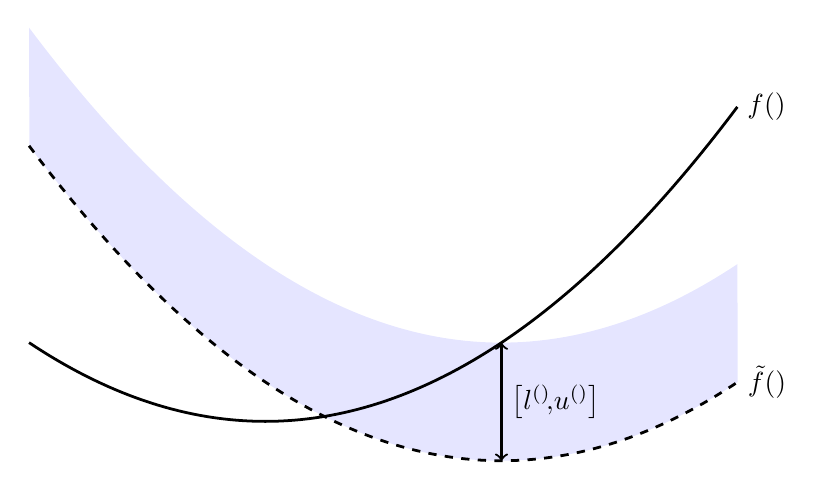
\begin{tikzpicture}[x=3cm, y=1cm]
					% Filled band around the quadratic curve with different boundary curves
					\fill[blue!10] 
					(-1, 5) -- plot[domain=-2:1, samples=100] ({\x+1}, {\x*\x + 1}) -- 
					plot[domain=1:-2, samples=100] ({\x+1}, {\x*\x - 0.5}) -- cycle;
					\node[anchor=west] at (2, 4) {$f(\weights)$};
					\draw[line width=1, domain=-2:1, samples=100,dashed] plot  ({\x+1}, {\x*\x -0.5}) node[right] {$\tilde{f}(\weights)$};
					\draw[line width=1, domain=-1:2, samples=100] plot ({\x}, {\x*\x});
					\draw[<->, thick] (1, -0.5) -- (1, 1) node[midway, right] {$\big[ l^{(\weights)}\!,\!u^{(\weights)} \big]$};
				\end{tikzpicture}
				\caption{\gls{ml} methods learn \gls{modelparams} $\weights$ by using some estimate of $f(\weights)$ for 
					the ultimate performance criterion $\bar{f}(\weights)$. Using a \gls{probmodel}, one can use $f(\weights)$ to 
					construct confidence intervals $\big[ l^{(\weights)},  u^{(\weights)} \big]$ which contain $\bar{f}(\weights)$  
					with high probability. The best plausible performance measure for a specific choice $\weights$ of \gls{modelparams} 
					is $\tilde{f}(\weights) \defeq l^{(\weights)}$.} 
			\end{center}
	\end{figure}},first={optimism in the face of uncertainty},text={optimism in the face of uncertainty} 
}


\newglossaryentry{dualnorm}
{name={dual norm},
	description={Every \gls{norm} $\normgeneric{\cdot}{}$ defined on an \gls{euclidspace} $\mathbb{R}^{\dimlocalmodel}$ 
		has an associated dual \gls{norm}, denoted $\normgeneric{\cdot}{*}$, defined as 
		$\normgeneric{\vy}{*} \defeq \sup_{\norm{\vx}{} \le 1} \vy^{T} \vx$. 
		The dual \gls{norm} measures the largest possible inner product between $\vy$ 
		and any vector in the unit ball of the original \gls{norm}. For further details, see 
		\cite[Sec.~A.1.6 ]{BoydConvexBook}.},
	first={dual norm},
	text={dual norm}
}

\newglossaryentry{geometricmedian}{
	name={geometric median (GM)},
	description={The GM\index{geometric median (GM)} of a set of input vectors $\vx^{(1)}, \ldots, \vx^{(\samplesize)}$ 
		in $\mathbb{R}^{\dimlocalmodel}$ is a point $\vz \in \mathbb{R}^{\dimlocalmodel}$ that 
		minimizes the sum of distances to the vectors \cite{BoydConvexBook} such that 
		\begin{equation} 
			\label{equ_geometric_median}
			\vz \in \argmin_{\vy \in \mathbb{R}^{\dimlocalmodel}} \sum_{\sampleidx=1}^{\samplesize} \normgeneric{\vy - \vx^{(\sampleidx)}}{2}.
		\end{equation} 
		\begin{figure}[H]
			\begin{center}
				\begin{tikzpicture}[scale=2, thick, >=stealth]
					%				% Central model w
					\coordinate (w) at (3,0);
					\fill (w) circle (1.2pt) node[below right] {$\vz$};
					% Good nodes
					\coordinate (w2) at (0.5,0.3);
					\coordinate (w3) at (0.7,0.7);
					\fill (w2) circle (1pt) node[above left] {$\vx^{(1)}$};
					\fill (w3) circle (1pt) node[above left] {$\vx^{(2)}$};
					%				%	\fill (wk) circle (1pt) node[above left] {$\mathbf{w}^{(k)}$};
					%				% Dashed lines from w to good nodes
					\draw[dashed] (w) -- (w2);
					\draw[dashed] (w) -- (w3);
					%				% Draw unit vectors (scaled to 1cm)
					\draw[->, thick, red] (w) -- ($(w)!1cm!(w2)$) ;
					\draw[->, thick, red] (w) -- ($(w)!1cm!(w3)$) node[pos=0.9, right,yshift=7pt] {$\frac{\vx^{(2)}- \vz}{\normgeneric{\vx^{(2)}-\vz}{2}}$};
					%				\node at (-0.2,1.4) {\textbf{Clean}};
					\coordinate (w4) at (5,0.2);
					\node at (5,0.4) {\textbf{Perturbed}};
					\fill (w4) circle (1pt) node[below left] {$\vx^{(3)}$};
					\draw[->, thick, red] (w) -- ($(w)!1cm!(w4)$) ;
					%		% Optional dotted line from w to bad
				\end{tikzpicture}
				\caption{\label{opt_cond_GM}
					Consider a solution $\vz$ of \eqref{equ_geometric_median} that does not coincide 
					with any of the input vectors. The optimality condition for \eqref{equ_geometric_median} 
					requires that the unit vectors from $\vz$ to the input vectors sum to zero.}
			\end{center}
		\end{figure}
		Figure~\ref{opt_cond_GM} illustrates a fundamental property of the GM:
		If $\vz$ does not coincide with any of the input vectors, then the unit vectors pointing 
		from $\vz$ to each $\vx^{(\sampleidx)}$ must sum to zero - this is the zero-\gls{subgradient}  
		(optimality) condition of \eqref{equ_geometric_median}. It turns out that the solution to 
		\eqref{equ_geometric_median} cannot be arbitrarily pulled away from trustworthy input vectors as long as they 
		are the majority \cite[Th. 2.2]{Lopuhaae1991}.},
	first={geometric median},
	text={GM}
}

\newglossaryentry{explanation}
{name={explanation},
	description={One approach to make \gls{ml} methods transparent is to provide an 
		explanation\index{explanation} along with the \gls{prediction} delivered by an 
		\gls{ml} method. Explanations can take on many different forms. An explanation 
		could be some natural text or some quantitative measure for the importance 
		of individual \gls{feature}s of a \gls{datapoint} \cite{Molnar2019}. We can also 
		use visual forms of explanations, such as intensity plots for image \gls{classification} \cite{GradCamPaper}.},
	first={explanation},text={explanation} 
}

\newglossaryentry{risk}
{name={risque},
	description={Consider\index{risque} a \gls{hypothesis} $\hypothesis$ used to predict the \gls{label} 
		$\truelabel$ of a \gls{datapoint} based on its \gls{feature}s $\featurevec$. We measure 
		the quality of a particular \gls{prediction} using a \gls{lossfunc} $\lossfunc{(\featurevec,\truelabel)}{\hypothesis}$. 
		If we interpret \gls{datapoint}s as the \gls{realization}s of \gls{iid} \gls{rv}s, 
		also the $\lossfunc{(\featurevec,\truelabel)}{\hypothesis}$ becomes the \gls{realization} 
		of an \gls{rv}. The \gls{iidasspt} allows us to define the risk of a \gls{hypothesis} 
		as the expected \gls{loss} $\expect \big\{\lossfunc{(\featurevec,\truelabel)}{\hypothesis} \big\}$. 
		Note that the risk of $\hypothesis$ depends on both the specific choice for the \gls{lossfunc} and the 
		\gls{probdist} of the \gls{datapoint}s.},
	first={risque},text={risque} 
}

\newglossaryentry{distributedalgorithm}
{name={distributed algorithm},
	description={A\index{distributed algorithm} distributed \gls{algorithm} is an \gls{algorithm} designed for 
		a special type of computer: a collection of interconnected computing devices (or nodes). 
		These devices communicate and coordinate their local computations by exchanging 
		messages over a network \cite{IntroDistAlg,ParallelDistrBook}. Unlike a classical \gls{algorithm}, 
		which is implemented on a single \gls{device}, a distributed \gls{algorithm} is 
		executed concurrently on multiple \gls{device}s with computational capabilities. 
		Similar to a classical \gls{algorithm}, a distributed \gls{algorithm} can be modeled as a 
		set of potential executions. However, each execution in the distributed setting involves 
		both local computations and message-passing events. A generic execution might look as 
		follows:
		\[
		\begin{array}{l}
			\text{Node 1: } {\rm input}_1, s_1^{(1)}, s_2^{(1)}, \ldots, s_{T_1}^{(1)}, {\rm output}_1; \\
			\text{Node 2: } {\rm input}_2, s_1^{(2)}, s_2^{(2)}, \ldots, s_{T_2}^{(2)}, {\rm output}_2; \\
			\quad \vdots \\
			\text{Node N: } {\rm input}_N, s_1^{(N)}, s_2^{(N)}, \ldots, s_{T_N}^{(N)}, {\rm output}_N.
		\end{array}
		\]
		Each \gls{device} $\nodeidx$ starts from its own local input and performs a sequence of 
		intermediate computations $s_{\iteridx}^{(\nodeidx)}$ at discrete time instants $\iteridx = 1, \dots, T_\nodeidx$. 
		These computations may depend on both: the previous local computations at the \gls{device} 
		and messages received from other \gls{device}s. One important application of distributed 
		\gls{algorithm}s is in \gls{fl} where a network of \gls{device}s collaboratively train a personal \gls{model} 
		for each \gls{device}. 
		},
	first={distributed algorithm}, text={distributed algorithm}
}


\newglossaryentry{algorithm}
{name={algorithme},
  description={An\index{algorithme} algorithm is a precise, step-by-step specification for 
  	how to produce an output from a given input within a finite number of computational steps \cite{Cormen:2022aa}. 
    For example, an algorithm for training a \gls{linmodel} explicitly describes how to 
	transform a given \gls{trainset} into \gls{modelparams} through a sequence of \gls{gradstep}s. 
    This informal characterization can be formalized rigorously via different mathematical \gls{model}s \cite{Sipser2013}. 
    One very simple \gls{model} of an algorithm is a collection of possible executions. Each execution is a sequence:
    $${\rm input},s_1,s_2,\ldots,s_T,{\rm output}$$ 
    that respects the constraints inherent to the computer executing the algorithm.
	Algorithms may be deterministic, where each input results uniquely in a single execution,
	or randomized, where executions can vary probabilistically. Randomized algorithms 
	can thus be analyzed by modeling execution sequences as outcomes of random experiments, 
	viewing the algorithm as a stochastic process \cite{RandomizedAlgos,BertsekasProb,Gallager13}.
	Crucially, an algorithm encompasses more than just a mapping from input to output; it also includes 
	the intermediate computational steps $s_1,\ldots,s_T$. 
	%. In \textbf{online algorithms}, these intermediate computational steps  can dynamically incorporate additional input data as the execution progresses.
	},
	first={algorithme},text={algorithme} 
}

\newglossaryentry{onlinelearning}
{name={online learning},
	description={
		Some \gls{ml} methods \index{online learning} are designed to process \gls{data} in a sequential 
		manner, updating their \gls{modelparams} as new \gls{datapoint}s become available—one at a time. 
		A typical example is time series data, such as daily minimum and maximum temperatures 
		recorded by a \gls{fmi} weather station. These values form a chronological sequence 
		of observations. In online learning, the \gls{hypothesis} (or its \gls{modelparams}) is refined 
		incrementally with each newly observed \gls{datapoint}, without revisiting past \gls{data}.  \\ 
		See also \gls{onlineGD}, \gls{onlinealgorithm}. 
	},
	first={online learning},text={online learning} 
}

\newglossaryentry{onlinealgorithm}
{name={online algorithm},
	description={An\index{online algorithm} online \gls{algorithm} processes input \gls{data} incrementally, 
		receiving \gls{datapoint}s sequentially and making decisions or producing outputs (or decisions) immediately 
		without having access to the entire input in advance \cite{PredictionLearningGames}, \cite{HazanOCO}. 
		Unlike an offline \gls{algorithm}, which has the entire input available from the start, an online \gls{algorithm} 
		must handle \gls{uncertainty} about future inputs and cannot revise past decisions. Similar to an 
		offline \gls{algorithm}, we also represent an online \gls{algorithm} formally as a collection of possible 
		executions. However, the execution sequence for an online \gls{algorithm} has a distinct structure:
		$${\rm in}_{1},s_1,{\rm out}_{1},{\rm in}_{2},s_2,{\rm out}_{2},\ldots,{\rm in}_{T},s_T,{\rm out}_{T}.$$ 
		Each execution begins from an initial state (i.e., \(\text{in}_{1}\)) and proceeds through alternating 
		computational steps, outputs (or decisions), and inputs. Specifically, at step \(\iteridx\), 
		the \gls{algorithm} performs a computational step \(s_{\iteridx}\), generates an output \(\text{out}_{\iteridx}\), 
		and then subsequently receives the next input (\gls{datapoint}) \(\text{in}_{\iteridx+1}\). A 
		notable example of an online \gls{algorithm} in \gls{ml} is \gls{onlineGD}, which incrementally 
		updates \gls{modelparams} as new \gls{datapoint}s arrive. 
		\\ See also: \gls{onlinelearning}, \gls{onlineGD}.
	},
	first={online algorithm},text={online algorithm} 
}



%\newglossaryentry{transparency}
%{name={transparency},
%	description={Transparency\index{transparency} is a key requirement for 
%		trustworthy \gls{ai} \cite{HLEGTrustworhtyAI}. In the context of ML methods, 
%		such as \gls{erm}-based methods, transparency is mainly used synonymously 
%		for \gls{explainability} \cite{gallese2023ai,JunXML2020}. However, in the wide 
%		context of \gls{ai} systems, transparency also includes providing information 
%		about limitations and reliability of the \gls{ai} system. As a point in case, \gls{logreg} provides a 
%		quantitative measure of the reliability of a \gls{classification} in the form of the value $|\hypothesis(\featurevec)|$. 
%		Transparency also includes the user interface, by requiring to clearly indicate when a user is 
%		interaction with an \gls{ai} system. Another component of transparency is the documentation 
%		of the system’s purpose, design choices, and intended use cases \cite{Shahriari2017,DatasheetData2021,10.1145/3287560.3287596}. },
%	first={transparency},text={transparency} 
%}

\newglossaryentry{transparency}
{name={transparency},
	description={Transparency\index{transparency} is a fundamental requirement for 
		\gls{trustAI} \cite{HLEGTrustworhtyAI}. In the context of \gls{ml} 
		methods, transparency is often used interchangeably with \gls{explainability} 
		\cite{gallese2023ai,JunXML2020}. However, in the broader scope of \gls{ai} 
		systems, transparency extends beyond \gls{explainability} and includes providing information 
		about the system’s limitations, reliability, and intended use. 
		In medical diagnosis systems, transparency requires disclosing the confidence level 
		for the \gls{prediction}s delivered by a trained \gls{model}. In credit scoring, 
		\gls{ai}-based lending decisions should be accompanied by explanations of 
		contributing factors, such as income level or credit history. These explanations 
		allow humans (e.g., a loan applicant) to understand and contest automated decisions. 
		Some \gls{ml} methods inherently offer transparency. For example, \gls{logreg} 
		provides a quantitative measure of \gls{classification} reliability through the value $|\hypothesis(\featurevec)|$. 
		\Gls{decisiontree}s are another example, as they allow human-readable decision rules \cite{rudin2019stop}.
		Transparency also requires a clear indication when a user is engaging with an \gls{ai} system. 
		For example, \gls{ai}-powered chatbots should notify users that they are interacting with an 
		automated system rather than a human. Furthermore, transparency encompasses comprehensive 
		documentation detailing the purpose and design choices underlying the \gls{ai} system. 
		For instance, \gls{model} datasheets \cite{DatasheetData2021} and \gls{ai} system cards \cite{10.1145/3287560.3287596} 
		help practitioners understand the intended use cases and limitations of an \gls{ai} system \cite{Shahriari2017}.},
	first={transparency}, text={transparency} 
}



\newglossaryentry{sensattr}
{name={sensitive attribute},
	description={\gls{ml}\index{sensitive attribute} revolves around learning a \gls{hypothesis} map that allows 
		us to predict the \gls{label} of a \gls{datapoint} from its \gls{feature}s. In some 
		applications, we must ensure that the output delivered by an \gls{ml} system does 
		not allow us to infer sensitive attributes of a \gls{datapoint}. Which part 
		of a \gls{datapoint} is considered a sensitive attribute is a design 
		choice that varies across different application domains.},
	first={sensitive attribute},text={sensitive attribute} 
}


\newglossaryentry{sbm}
{name={stochastic block model (SBM)},
	description={The\index{stochastic block model (SBM)} stochastic block \gls{model} is a 
		probabilistic generative \gls{model} for an undirected \gls{graph} $\graph = \big( \nodes, \edges \big)$ 
		with a given set of nodes $\nodes$ \cite{AbbeSBM2018}. In its most basic variant, 
		the stochastic block \gls{model} generates a \gls{graph} by first randomly assigning each node $\nodeidx \in \nodes$ to 
		a \gls{cluster} index $\clusteridx_{\nodeidx} \in \{1,\ldots,\nrcluster\}$. A pair of different nodes in the 
		\gls{graph} is connected by an edge with \gls{probability} $p_{\nodeidx,\nodeidx'}$ that depends 
		solely on the \gls{label}s $\clusteridx_{\nodeidx}, \clusteridx_{\nodeidx'}$. 
		The presence of edges between different pairs of 
		nodes is statistically independent. },
	first={stochastic block model (SBM)},text={SBM} 
}

\newglossaryentry{deepnet}
{name={deep net},
	description={A\index{deep net} deep net is an \gls{ann} with a (relatively) large number of 
	hidden layers. Deep learning is an umbrella term for \gls{ml} methods that use a deep 
	net as their \gls{model} \cite{Goodfellow-et-al-2016}.},
	first={deep net},text={deep net} 
}

\newcommand{\gaussiancenter}{3}

\newglossaryentry{baseline}
{name={baseline},
    description={Consider\index{baseline} some \gls{ml} method that produces a learned 
    	\gls{hypothesis} (or trained \gls{model}) $\learnthypothesis \in \hypospace$. We evaluate the quality of a trained \gls{model} 
    by computing the average \gls{loss} on a \gls{testset}. But how can we assess 
    whether the resulting \gls{testset} performance is sufficiently good? How can we 
    determine if the trained \gls{model} performs close to optimal and there is little point 
    in investing more resources (for \gls{data} collection or computation) to improve it? 
    To this end, it is useful to have a reference (or baseline) level against which 
    we can compare the performance of the trained \gls{model}. Such a reference value 
    might be obtained from human performance, e.g., the misclassification rate of dermatologists 
    who diagnose cancer from visual inspection of skin \cite{SkinHumanAI}. Another source for a baseline is an existing, 
    but for some reason unsuitable, \gls{ml} method. For example, the existing \gls{ml} method 
    might be computationally too expensive for the intended \gls{ml} application. 
    Nevertheless, its \gls{testset} error can still serve as a baseline. Another, somewhat more principled, 
    approach to constructing a baseline is via a \gls{probmodel}. In many cases, given a \gls{probmodel} $p(\featurevec,\truelabel)$,  
    we can precisely determine the \gls{minimum} achievable \gls{risk} among any hypotheses
    (not even required to belong to the \gls{hypospace} $\hypospace$) \cite{LC}. 
    This \gls{minimum} achievable \gls{risk} (referred to as the \gls{bayesrisk}) is the \gls{risk} 
    of the \gls{bayesestimator} for the \gls{label} $\truelabel$ of a \gls{datapoint}, given
    its \gls{feature}s $\featurevec$. Note that, for a given choice of \gls{lossfunc}, the 
    \gls{bayesestimator} (if it exists) is completely determined by the \gls{probdist} $p(\featurevec,\truelabel)$ \cite[Ch. 4]{LC}. 
    However, computing the \gls{bayesestimator} and \gls{bayesrisk} presents two 
    main challenges:
    \begin{enumerate}[label=\arabic*)]
    	\item The \gls{probdist} $p(\featurevec,\truelabel)$ is unknown and 
    needs to be estimated.
    	\item Even if $p(\featurevec,\truelabel)$ is known, 
    it can be computationally too expensive to compute the \gls{bayesrisk} exactly \cite{cooper1990computational}. 
   \end{enumerate}
A widely used \gls{probmodel} is the \gls{mvndist} $\pair{\featurevec}{\truelabel} \sim \mathcal{N}({\bm \mu},{\bm \Sigma})$ 
for \gls{datapoint}s characterized by numeric \gls{feature}s and \gls{label}s.
Here, for the \gls{sqerrloss}, the \gls{bayesestimator} is given by the posterior 
\gls{mean} $\mu_{\truelabel|\featurevec}$ of the \gls{label} $\truelabel$, given the 
\gls{feature}s $\featurevec$ \cite{LC,GrayProbBook}. The corresponding \gls{bayesrisk} 
is given by the posterior \gls{variance} 
$\sigma^{2}_{\truelabel|\featurevec}$ (see Figure \ref{fig_post_baseline_dict}).
	\begin{figure}[H]
		\begin{center}
		\begin{tikzpicture}
			% Axes
			\draw[->] (-1,0) -- (7,0) node[right] {$\truelabel$}; % x-axis
			% Gaussian distribution centered at \gaussiancenter with variance 1
			\draw[thick,domain=-1:7,smooth,variable=\x] 
			  plot ({\x}, {2*exp(-0.5*((\x-\gaussiancenter)^2))});
			% Dashed line indicating the mean of the Gaussian
			\draw[dashed] (\gaussiancenter,0) -- (\gaussiancenter,2.5);
			\node[anchor=south] at ([yshift=-5pt] \gaussiancenter,2.5) {\small $\mu_{\truelabel|\featurevec}$};
			% Double arrow indicating the variance
			\draw[<->,thick] (\gaussiancenter-1,1) -- (\gaussiancenter+1,1.0);
			\node[anchor=west] at ([yshift=2pt] \gaussiancenter,1.2) {\small $\sigma_{\truelabel|\featurevec}$};
			% Posterior variance label
			%\node[anchor=south east] at (\gaussiancenter-0.5,1.8) {\small Posterior Variance};
			% x-axis marks with crosses
			  % x-axis marks with crosses
  			\foreach \x in {0.5} {
				\node[red] at (\x, 0) {\bf \large $\times$};
 			 }
  % h(x) label for the first cross
  			\node[anchor=north] at (0.5,-0.2) {\small $\learnthypothesis(\featurevec)$};
		  \end{tikzpicture}
		\end{center}
		\caption{If the \gls{feature}s and the \gls{label} of a \gls{datapoint} are drawn from a \gls{mvndist}, we 
		can achieve the \gls{minimum} \gls{risk} (under \gls{sqerrloss}) by using the \gls{bayesestimator} $\mu_{\truelabel|\featurevec}$ 
		to predict the \gls{label} $\truelabel$ of a \gls{datapoint} with \gls{feature}s $\featurevec$. The corresponding 
		\gls{minimum} \gls{risk} is given by the posterior \gls{variance} $\sigma^{2}_{\truelabel|\featurevec}$. We can use 
		this quantity as a baseline for the average \gls{loss} of a trained \gls{model} $\learnthypothesis$. \label{fig_post_baseline_dict}}
	\end{figure}},
    first={baseline},text={baseline}
}

\newglossaryentry{spectrogram}
{name={spectrogram},
	description={
		A\index{spectrogram} spectrogram represents the time-frequency distribution of the energy of a time signal $x(t)$.  
		Intuitively, it quantifies the amount of signal energy present within a specific time segment 
		$[t_{1},t_{2}] \subseteq \mathbb{R}$ and frequency interval $[f_{1},f_{2}]\subseteq \mathbb{R}$. 
		Formally, the spectrogram of a signal is defined as the squared magnitude of its 
		short-time Fourier transform (STFT) \cite{cohen1995time}.
        Figure \ref{fig:spectrogram_dict} depicts a time signal along with its spectrogram. 
	\begin{figure}[H]
		\centering
		\includegraphics[width=0.8\textwidth]{../../assets/spectrogram.png}
		\caption{Left: A time signal consisting of two modulated Gaussian pulses. Right: An intensity 
		plot of the spectrogram.
		\label{fig:spectrogram_dict}}
	\end{figure}
        The intensity plot of its spectrogram can serve as an image of a signal. A 
		simple recipe for audio signal \gls{classification} is to feed this signal image 
		into \gls{deepnet}s originally developed for image \gls{classification} and object detection \cite{Li:2022aa}. 
		It is worth noting that, beyond the spectrogram, several alternative representations exist 
		for the time-frequency distribution of signal energy \cite{TimeFrequencyAnalysisBoashash,MallatBook}. 
		}, 
	first={spectrogram},text={spectrogram} 
}

\newglossaryentry{graphclustering}
{name={graph clustering},
	description={\Gls{graph} \gls{clustering}\index{graph clustering} aims at 
		\gls{clustering} \gls{datapoint}s that are represented as the nodes 
		of a \gls{graph} $\graph$. The edges of $\graph$ represent 
		pairwise similarities between \gls{datapoint}s. Sometimes we
		can quantify the extend of these similarities by an \gls{edgeweight} \cite{Luxburg2007,FlowSpecClustering2021}. }, 
	first={graph clustering},text={graph clustering} 
}

\newglossaryentry{specclustering}
{name={spectral clustering},
	description={Spectral \gls{clustering}\index{spectral clustering} is a particular instance of 
		\gls{graphclustering}, i.e., it clusters \gls{datapoint}s 
		represented as the nodes $\nodeidx=1,\ldots,\nrnodes$ of a \gls{graph} $\graph$. 
		Spectral \gls{clustering} uses the \gls{eigenvector}s of the \gls{LapMat} $\LapMat{\graph}$ 
		to construct \gls{featurevec}s $\featurevec^{(\nodeidx)} \in \mathbb{R}^{\nrfeatures}$ 
		for each node (i.e., for each \gls{datapoint}) $\nodeidx=1,\ldots,\nrnodes$. We can feed these \gls{featurevec}s 
		into \gls{euclidspace}-based \gls{clustering} methods, such as \gls{kmeans} 
		or \gls{softclustering} via \gls{gmm}. Roughly speaking, the \gls{featurevec}s of nodes 
		belonging to a well-connected subset (or \gls{cluster}) of nodes in $\graph$ are located 
		nearby in the \gls{euclidspace} $\mathbb{R}^{\nrfeatures}$ (see Figure \ref{fig_lap_mtx_specclustering_dict}). 
		\begin{figure}[H]
			\begin{center}
				\begin{minipage}{0.4\textwidth}
			\begin{tikzpicture}
				% Define the style for filled nodes
				\begin{scope}[every node/.style={circle, fill=black, inner sep=0pt, minimum size=0.3cm}]
					% Define nodes
					\node (1) at (0,0) {};
					\node (2) [below left=of 1, xshift=-0.2cm, yshift=-1cm] {};
					\node (3) [below right=of 1, xshift=0.2cm, yshift=-1cm] {};
					\node (4) [below=of 1, yshift=0.5cm] {}; % Isolated node
				\end{scope}
				% Draw edges
				\draw (1) -- (2);
				\draw (1) -- (3);
				% Add labels (separate from filled nodes)
				\node[above=0.2cm] at (1) {$\nodeidx=1$};
				\node[left=0.3cm] at (2) {$2$};
				\node[right=0.3cm] at (3) {$3$};
				\node[below=0.2cm] at (4) {$4$};
			\end{tikzpicture}
				\end{minipage} 
				\hspace*{5mm}
				\begin{minipage}{0.4\textwidth}
					\begin{equation} 
						\LapMat{\graph}\!=\!
						\begin{pmatrix} 
							2 & -1 & -1 & 0 \\ 
							-1 & 1 & 0 & 0 \\  
							-1 & 0 & 1 & 0 \\ 
							0 & 0 & 0 & 0 
						\end{pmatrix}\!=\!\mathbf{V} {\bm \Lambda} \mathbf{V}^{T}  
						\nonumber
					\end{equation} 
				\end{minipage}
				\vspace*{20mm}\\
				  \begin{minipage}{0.4\textwidth}
				\begin{tikzpicture}[scale=3]
%					% Axes
					\draw[->] (-0.2, 0) -- (1.2, 0) node[right] {$v^{(1)}_{\nodeidx}$};
					\draw[->] (0, -0.2) -- (0, 1.2) node[above] {$v^{(2)}_{\nodeidx}$};
%					
%					% Tailored tick marks and labels
%					\draw (0,0) node[below left] {$0$};
%					\draw (1/sqrt(3), 0) node[below] {$\frac{1}{\sqrt{3}}$} -- ++(0,0.05);
%					\draw (0, 1) node[left] {$1$} -- ++(0.05,0);
%					
%					 Data points
					\filldraw[blue] (0.577, 0) circle (0.03cm) node[above right] {$\nodeidx=1,2,3$};
					\filldraw[blue] (0.577, 0) circle (0.03cm); % Second point overlaps
					\filldraw[blue] (0.577, 0) circle (0.03cm); % Third point overlaps
					\filldraw[red] (0, 1) circle (0.03cm) node[above right] {$4$};
%					% Grid for reference
%					\draw[dashed, gray] (1/sqrt(3), 0) -- (1/sqrt(3), 1);
%					\draw[dashed, gray] (0, 1) -- (1, 1);
				\end{tikzpicture}
				\end{minipage} 
    		\begin{minipage}{0.4\textwidth}
										\begin{align}
											& \mathbf{V} = \big( \vv^{(1)},\vv^{(2)},\vv^{(3)},\vv^{(4)} \big) \nonumber \\
											&	\mathbf{v}^{(1)}\!=\!\frac{1}{\sqrt{3}} \begin{pmatrix} 1 \\ 1 \\ 1 \\ 0 \end{pmatrix}, \,
												\mathbf{v}^{(2)}\!=\!\begin{pmatrix} 0 \\ 0 \\ 0 \\ 1 \end{pmatrix} \nonumber 
										\end{align}
				\end{minipage} 
				\caption{\label{fig_lap_mtx_specclustering_dict} {\bf Top.} Left: An undirected \gls{graph} 
					$\graph$ with four nodes $\nodeidx=1,2,3,4$, each representing a \gls{datapoint}. Right: The \gls{LapMat} 
					$\LapMat{\graph}  \in \mathbb{R}^{4 \times 4}$ and its \gls{evd}. 
					{\bf Bottom.} Left: A \gls{scatterplot} of \gls{datapoint}s using the \gls{featurevec}s 
					$\featurevec^{(\nodeidx)} = \big( v^{(1)}_{\nodeidx},v^{(2)}_{\nodeidx} \big)^{T}$. 
					Right: Two \gls{eigenvector}s $\vv^{(1)},\vv^{(2)} \in \mathbb{R}^{\nrfeatures}$ 
					corresponding to the \gls{eigenvalue} $\lambda=0$ of the \gls{LapMat} $\LapMat{\graph}$. 
					} 
			\end{center}
		\end{figure}
	\newpage}, 
	first={spectral clustering},text={spectral clustering} 
}

\newglossaryentry{flowbasedclustering}
{name={flow-based clustering},
	description={Flow-based \gls{clustering}\index{flow-based clustering} groups the nodes 
		of an undirected \gls{graph} by applying \gls{kmeans} \gls{clustering} to node-wise 
		\gls{featurevec}s. These \gls{featurevec}s are built from network flows between 
		carefully selected sources and destination nodes \cite{FlowSpecClustering2021}. }, 
	first={flow-based clustering},text={flow-based clustering} 
}



\newglossaryentry{esterr}
{name={estimation error},
	description={Consider\index{estimation error} \gls{datapoint}s, each with \gls{featurevec} $\featurevec$ and \gls{label} 
		$\truelabel$. In some applications, we can model the relation between the \gls{featurevec} and the \gls{label}
		of a \gls{datapoint} as $\truelabel = \bar{\hypothesis}(\featurevec) + \varepsilon$. Here, we 
		use some true underlying \gls{hypothesis} $\bar{\hypothesis}$ and a noise term $\varepsilon$ 
		which summarizes any modeling or labeling errors. The estimation error incurred by an \gls{ml} 
		method that learns a \gls{hypothesis} $\widehat{\hypothesis}$, e.g., using \gls{erm}, is defined as 
		$\widehat{\hypothesis}(\featurevec) - \bar{\hypothesis}(\featurevec)$, for some \gls{featurevec}. 
		For a parametric \gls{hypospace}, which consists of \gls{hypothesis} maps determined by 
		\gls{modelparams} $\weights$, we can define the estimation error as $\Delta \weights = \widehat{\weights} - \overline{\weights}$ \cite{kay,hastie01statisticallearning}.},
	first={estimation error},text={estimation error} 
}


\newglossaryentry{dob}
{name={degree of belonging},
	description={Degree of belonging\index{degree of belonging} is a number that indicates the extent to which a \gls{datapoint} 
		belongs to a \gls{cluster} \cite[Ch. 8]{MLBasics}. The degree of belonging can be 
		interpreted as a soft \gls{cluster} assignment. \Gls{softclustering} methods can 
		encode the degree of belonging by a real number in the interval $[0,1]$. 
		\Gls{hardclustering} is obtained as the extreme case when the degree of belonging 
		only takes on values $0$ or $1$.}, first={degree of belonging},text={degree of belonging} 
}

\newglossaryentry{msee}
{name={mean squared estimation error (MSEE)},
	description={Consider\index{mean squared estimation error (MSEE)} an \gls{ml} method that 
		learns \gls{modelparams} $\widehat{\weights}$ based on some \gls{dataset} $\dataset$. 
		If we interpret the \gls{datapoint}s in $\dataset$ as \gls{iid} \gls{realization}s of an \gls{rv} $\datapoint$, 
		we define the \gls{esterr} $\Delta \weights \defeq \widehat{\weight} - \overline{\weights}$. 
		Here, $\overline{\weights}$ denotes the true \gls{modelparams} of the \gls{probdist} 
		of $\datapoint$. The \gls{mean} squared \gls{esterr} is 
		defined as the \gls{expectation} $\expect \big\{ \big\| \Delta \weights \big\|^{2} \big\}$ of the 
		squared Euclidean \gls{norm} of the \gls{esterr} \cite{LC,kay}.},
	first={mean squared estimation error (MSEE)},text={MSEE} 
}

\newglossaryentry{gtvmin}
{name={generalized total variation minimization (GTVMin)},
	description={\gls{gtv} minimization\index{generalized total variation minimization (GTVMin)} is an instance of \gls{rerm} 
		using the \gls{gtv} of local \gls{modelparams} as a \gls{regularizer} \cite{ClusteredFLTVMinTSP}.},
	first={generalized total variation minimization (GTVMin)},text={GTVMin} 
}


\newglossaryentry{acc}
{name={accuracy},
	description={Consider\index{accuracy} \gls{datapoint}s characterized by \gls{feature}s $\featurevec \in \featurespace$ and 
		a categorical label $\truelabel$ which takes on values from a finite \gls{labelspace} $\labelspace$. The 
		accuracy of a \gls{hypothesis} $\hypothesis: \featurespace \rightarrow \labelspace$, when applied 
		to the \gls{datapoint}s in a \gls{dataset} $\dataset = \big\{ \big(\featurevec^{(1)}, \truelabel^{(1)} \big), \ldots, \big(\featurevec^{(\samplesize)},\truelabel^{(\samplesize)}\big) \big\}$, 
		is then defined as $1 - (1/\samplesize)\sum_{\sampleidx=1}^{\samplesize} \lossfunczo{\big(\featurevec^{(\sampleidx)},\truelabel^{(\sampleidx)}\big)}{\hypothesis}$ using the \gls{zerooneloss} $\lossfunczo{\cdot}{\cdot}$.},
	first={accuracy},text={accuracy} 
}





\newglossaryentry{expert}
{name={expert},
	description={\gls{ml}\index{expert} aims to learn a \gls{hypothesis} $\hypothesis$ that accurately predicts the \gls{label} 
		of a \gls{datapoint} based on its \gls{feature}s. We measure the \gls{prediction} error using 
		some \gls{lossfunc}. Ideally, we want to find a \gls{hypothesis} that incurs minimal \gls{loss} 
		on any \gls{datapoint}. We can make this informal goal precise via the \gls{iidasspt} 
		and by using the \gls{bayesrisk} as the \gls{baseline} for the (average) \gls{loss} of a \gls{hypothesis}. 
		An alternative approach to obtaining a \gls{baseline} is to use the \gls{hypothesis} $\hypothesis'$ learned 
		by an existing \gls{ml} method. We refer to this \gls{hypothesis} $\hypothesis'$ as an expert \cite{PredictionLearningGames}. \Gls{regret} minimization methods learn a \gls{hypothesis}
		that incurs a \gls{loss} comparable to the best expert \cite{PredictionLearningGames,HazanOCO}.},
	first={expert},text={expert} 
}

\newglossaryentry{nfl}
{name={networked federated learning (NFL)},
	description={Networked \gls{fl}\index{networked federated learning (NFL)} refers 
		to methods that learn personalized \gls{model}s in a distributed fashion. These methods learn from \gls{localdataset}s 
		that are related by an intrinsic network structure.},
 first={networked federated learning (NFL)},text={NFL} 
}




\newglossaryentry{regret}
{name={regret},
	description={The regret\index{regret} of a \gls{hypothesis} $\hypothesis$ relative to 
		another \gls{hypothesis} $\hypothesis'$, which serves as a \gls{baseline}, 
		is the difference between the \gls{loss} incurred by $\hypothesis$ and the \gls{loss} 
		incurred by $\hypothesis'$ \cite{PredictionLearningGames}. 
		The \gls{baseline} \gls{hypothesis} $\hypothesis'$ is also referred to as an \gls{expert}.},
	first={regret},text={regret} 
}

\newglossaryentry{strcvx}
{name={strongly convex},
	description={A\index{strongly convex} continuously \gls{differentiable} real-valued 
		function $f(\featurevec)$ is strongly \gls{convex} with coefficient $\sigma$ if $f(\vy) \geq f(\vx) + \nabla f(\vx)^{T} (\vy - \vx) + (\sigma/2) \normgeneric{\vy - \vx}{2}^{2}$ \cite{nesterov04},\cite[Sec. B.1.1]{CvxAlgBertsekas}.},
	first={strongly convex},text={strongly convex} 
}

\newglossaryentry{subgradient}
{name={subgradient},
description={For\index{subgradient} a real-valued function $f: \mathbb{R}^{\featuredim} \rightarrow \mathbb{R}: \weights \mapsto f(\weights)$, 
		a vector $\va$ such that $f(\weights) \geq  f(\weights') +\big(\weights-\weights' \big)^{T} \va$ is 
		referred to as a subgradient of $f$ at $\weights'$ \cite{BertCvxAnalOpt,BertsekasNonLinProgr}.},
	first={subgradient},text={subgradient} 
}

\newglossaryentry{FedRelax}
{name={FedRelax},
	description={An\index{FedRelax} \gls{fl} \gls{distributedalgorithm}. 
		\\ 
		See also: \gls{fl}, \gls{algorithm}.},
	first={FedRelax},text={FedRelax}
} 

\newglossaryentry{fedavg}
{name={FedAvg},
	description={FedAvg\index{FedAvg} refers to a family of iterative \gls{fl} \glspl{algorithm}. 
		It uses a server-client setting and alternatves between client-wise \glspl{localmodel} 
		re-training, followed by the aggregation of updated \gls{modelparams} at the server 
		\cite{pmlr-v54-mcmahan17a}.  
		\\ 
		See also: \gls{fl}, \gls{algorithm}.},
	first={FedAvg},text={FedAvg}
} 

\newglossaryentry{fedprox}
{name={FedProx},
	description={FedProx\index{FedProx} refers to an iterative \gls{fl} \gls{algorithm} that alternates between separately training \gls{localmodel}s and combining the updated local \gls{modelparams}. In contrast to \gls{fedavg}, which uses 
		\gls{stochGD} to train \gls{localmodel}s, FedProx uses a \gls{proxop} for the training \cite{FedProx2020}.}, 
	first = {FedProx}, text={FedProx} 
}

\newglossaryentry{relu}
{name={rectified linear unit (ReLU)},
	description={The\index{rectified linear unit (ReLU)} ReLU is 
		a popular choice for the \gls{actfun} of a neuron within an \gls{ann}. It is defined 
		as $\actfun(z) = \max\{0,z\}$, with $z$ being the weighted input of the artificial 
		neuron.}, first = {rectified linear unit (ReLU)}, text={ReLU} 
}



\newglossaryentry{vcdim}
{name={Vapnik–Chervonenkis dimension (VC dimension)},
	description={The\index{Vapnik–Chervonenkis dimension (VC dimension)} VC dimension of an infinite \gls{hypospace} is a widely-used measure 
		for its size. We refer to the literature (see \cite{ShalevMLBook}) for a precise definition of VC dimension 
		as well as a discussion of its basic properties and use in \gls{ml}.},
	first={Vapnik–Chervonenkis dimension (VC dimension)},text={VC dimension}  
}

\newglossaryentry{labelspace}
{name={label space},
	description={Consider\index{label space} an \gls{ml} application that involves \glspl{datapoint} characterized by \glspl{feature} 
		and \glspl{label}. The \gls{label} space is constituted by all potential values that the \gls{label} 
		of a \gls{datapoint} can take on. \Gls{regression} methods, aiming at predicting numeric \glspl{label}, often
		use the \gls{label} space $\labelspace = \mathbb{R}$. Binary \gls{classification} methods use a \gls{label} space 
		that consists of two different elements, e.g., $\labelspace =\{-1,1\}$, $\labelspace=\{0,1\}$, 
		or .
		\\ 
		See also: \gls{ml}, \gls{datapoint}, \gls{feature}, \gls{label}, \gls{regression}, \gls{classification}.}, 
	first={label space},
	text={label space}  
}


\newglossaryentry{histogram}
{name={histogram},
	description={Consider\index{histogram} a \gls{dataset} $\dataset$ that consists of $\samplesize$ \gls{datapoint}s 
		$\datapoint^{(1)},\ldots,\datapoint^{(\samplesize)}$, each of them belonging to some 
		cell $[-U,U] \times \ldots \times [-U,U] \subseteq \mathbb{R}^{\featuredim}$ with side 
		length $U$. We partition this cell evenly into smaller elementary cells with side 
		length $\Delta$. The histogram of $\dataset$ assigns each elementary cell to 
		the corresponding fraction of \gls{datapoint}s in $\dataset$ that fall into this 
		elementary cell. A visual example of such a histogram is provided in Figure~\ref{fig:histogram}.\\		
		\begin{figure}
			\centering
			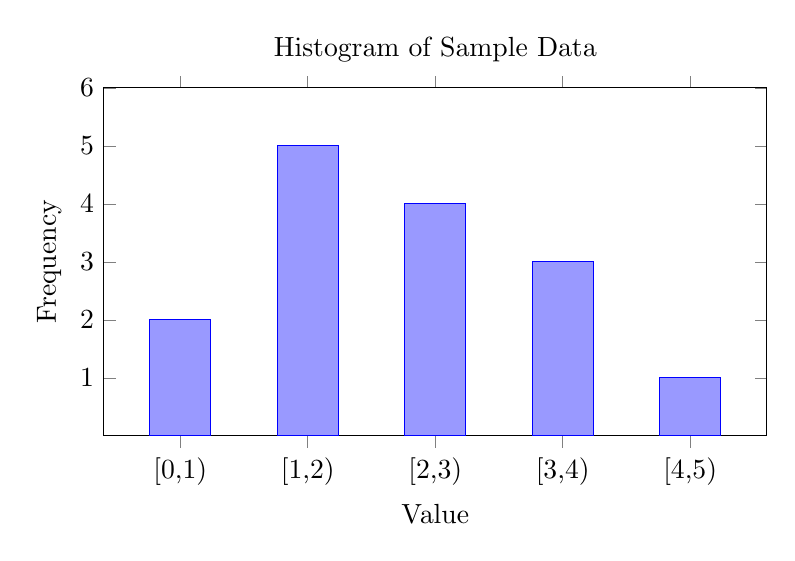
\begin{tikzpicture}
				\pgfplotsset{compat=1.18}
				\begin{axis}[
					ybar,
					ymin=0,
					ymax=6,
					bar width=22pt,
					width=10cm,
					height=6cm,
					xlabel={Value},
					ylabel={Frequency},
					ytick={1,2,3,4,5,6},
					xtick={1,2,3,4,5},
					xticklabels={{[0,1)}, {[1,2)}, {[2,3)}, {[3,4)}, {[4,5)}},
					enlarge x limits=0.15,
					title={Histogram of Sample Data}
					]
					\addplot+[fill=blue!40] coordinates {(1,2) (2,5) (3,4) (4,3) (5,1)};
				\end{axis}
			\end{tikzpicture}
			\caption{A histogram representing the frequency of data points falling within discrete value ranges (bins). Each bar height shows 		the count of samples in the corresponding interval.}
			\label{fig:histogram}
		\end{figure}
	},
	first={histogram},text={histogram}  
}

\newglossaryentry{bootstrap}
{name={bootstrap},
	description={For\index{bootstrap} the analysis of \gls{ml} methods, it is often useful to interpret 
		a given set of \gls{datapoint}s $\dataset = \big\{ \datapoint^{(1)},\ldots,\datapoint^{(\samplesize)}\big\}$ 
		as \gls{realization}s of \gls{iid} \gls{rv}s with a common \gls{probdist} $p(\datapoint)$. In general, we 
		do not know $p(\datapoint)$ exactly, but we need to estimate it. The bootstrap uses the 
		histogram of $\dataset$ as an estimator for the underlying \gls{probdist} $p(\datapoint)$. 
	},
	first={bootstrap},text={bootstrap}  
}



\newglossaryentry{missingdata}
{name={missing data},
	description={Consider\index{missing data} a \gls{dataset} constituted by \gls{datapoint}s collected via 
		some physical \gls{device}. Due to imperfections and failures, some of the \gls{feature} 
		or \gls{label} values of \gls{datapoint}s might be corrupted or simply missing. 
		\Gls{data} imputation aims at estimating these missing values \cite{Abayomi2008DiagnosticsFM}. 
		We can interpret \gls{data} imputation as an \gls{ml} problem where the \gls{label} of a \gls{datapoint} is 
		the value of the corrupted \gls{feature}. },
	first={missing data},text={missing data}  
}


\newglossaryentry{predictor}
{name={predictor},
	description={A\index{predictor} predictor is a real-valued \gls{hypothesis} map. 
		Given a \gls{datapoint} with \gls{feature}s $\featurevec$, the value 
		$\hypothesis(\featurevec) \in \mathbb{R}$ is used as a \gls{prediction} for the true 
		numeric \gls{label} $\truelabel \in \mathbb{R}$ of the \gls{datapoint}. },first={predictor},text={predictor}  
}

\newglossaryentry{labeled datapoint}
{name={labeled datapoint},
 description={A\index{labeled datapoint} \gls{datapoint} whose \gls{label} is known or has been determined 
 	by some means which might require human labor.},
 first={labeled datapoint},text={labeled datapoint}  
}



\newglossaryentry{netmodel}
{name={networked model},
  description={A\index{networked model} networked \gls{model} over an \gls{empgraph} $\graph = \pair{\nodes}{\edges}$ assigns 
   a \gls{localmodel} (i.e., a \gls{hypospace}) to each node $\nodeidx \in \nodes$ of the \gls{empgraph} $\graph$.}, 
   first={networked model},text={networked model}  
}


\newglossaryentry{netdata}
{
	name={networked data},
	description={Networked\index{networked data} \gls{data} consists of \gls{localdataset}s 
	that are related by some notion of pairwise similarity. We can represent networked 
	\gls{data} using a \gls{graph} whose nodes carry \gls{localdataset}s and edges encode 
	pairwise similarities. One example of networked \gls{data} arises in \gls{fl} applications 
	where \gls{localdataset}s are generated by spatially distributed \gls{device}s.}, 
	first={networked data},text={networked data}  
}

\newglossaryentry{validation} 
{name={validation},
	description={Consider\index{validation} a \gls{hypothesis} $\learnthypothesis$ that has been 
		learned via some \gls{ml} method, e.g., by solving \gls{erm} on a \gls{trainset} $\dataset$. 
		Validation refers to the practice of evaluating the \gls{loss} incurred by the 
		\gls{hypothesis} $\learnthypothesis$ on a set of 
		\gls{datapoint}s that are not contained in the \gls{trainset} $\dataset$. },first={validation},text={validation}  
}

\newglossaryentry{quadfunc}
{name={quadratic function},
	description={A\index{quadratic function} function $f: \mathbb{R}^{\nrfeatures} \rightarrow \mathbb{R}$ of the form 
	$$f(\weights) =  \weights^{T} \mathbf{Q} \mathbf{w} + \mathbf{q}^{T} \weights+a,$$ with 
	some matrix $\mQ \in \mathbb{R}^{\nrfeatures \times \nrfeatures}$, vector $\vq \in \mathbb{R}^{\nrfeatures}$, 
	and scalar $a \in \mathbb{R}$.  },first={quadratic function},text={quadratic function}  
}

\newglossaryentry{testset}
{name={ensemble de test (ou jeu de test)},
	description={A\index{ensemble de test (ou jeu de test)} set of \gls{datapoint}s that have  
		been used neither to train a \gls{model} (e.g., via \gls{erm}) nor in a \gls{valset} 
		to choose between different \gls{model}s.},first={ensemble de test (ou jeu de test)},text={ensemble de test}  
}


\newglossaryentry{modelsel}
{name={model selection},
	description={In\index{model selection} \gls{ml}, \gls{model} selection refers to the 
		process of choosing between different candidate \gls{model}s. In its most 
		basic form, \gls{model} selection amounts to: 1) training each candidate \gls{model}; 
		2) computing the \gls{valerr} for each trained \gls{model}; and 3) choosing the \gls{model} 
		with the smallest \gls{valerr} \cite[Ch. 6]{MLBasics}. },first={model selection},text={model selection}  
}





\newglossaryentry{linclass}{name={linear classifier}, description={
	    Consider\index{linear classifier} \gls{datapoint}s characterized by numeric \gls{feature}s $\featurevec \in \mathbb{R}^{\nrfeatures}$ 
	    and a \gls{label} $\truelabel \in \labelspace$ from some finite \gls{labelspace} $\labelspace$. 
		A linear \gls{classifier} is characterized by having \gls{decisionregion}s that are 
		separated by hyperplanes in $\mathbb{R}^{\featuredim}$ \cite[Ch. 2]{MLBasics}.},first={linear classifier},text={linear classifier} }

\newglossaryentry{multilabelclass}{name={classification multi-classe}, description={Multi-\gls{label} 
		\gls{classification}\index{classification multi-classe} problems and methods use \gls{datapoint}s 
		that are characterized by several \gls{label}s. As an example, consider a \gls{datapoint} 
		representing a picture with two \gls{label}s. One \gls{label} indicates the presence of a human 
		in this picture and another \gls{label} indicates the presence of a car.},
	    first={classification multi-classe},text={classification multi-classe} }


\newglossaryentry{ssl}{
	name={apprentissage semi-supervisé}, 
	description={SSL\index{apprentissage semi-supervisé} methods use unlabeled \gls{datapoint}s 
		to support the learning of a \gls{hypothesis} from \gls{labeled datapoint}s \cite{SemiSupervisedBook}. 
		This approach is particularly useful for \gls{ml} applications that offer a large amount of 
		unlabeled \gls{datapoint}s, but only a limited number of \gls{labeled datapoint}s.}, 
	first={apprentissage semi-supervisé},text={apprentissage semi-supervisé} }
	
	
\newglossaryentry{objfunc}{name={objective function}, description={An\index{objective function} 
		objective function is a map that assigns each value of an optimization variable, such 
		as the \gls{modelparams} $\weights$ of a \gls{hypothesis} $\hypothesis^{(\weights)}$, to 
		an objective value $f(\weights)$. The objective value $f(\weights)$ could be the 
		\gls{risk} or the \gls{emprisk} of a \gls{hypothesis} $\hypothesis^{(\weights)}$.},first={objective function},text={objective function} }
	
\newglossaryentry{regularizer}{name={regularizer}, description={A regularizer\index{regularizer} 
		assigns each \gls{hypothesis} $\hypothesis$ from a \gls{hypospace} $\hypospace$ a quantitative 
		measure $\regularizer{\hypothesis}$ for how much its \gls{prediction} error on a \gls{trainset} might 
		differ from its \gls{prediction} errors on \gls{datapoint}s outside the \gls{trainset}. \Gls{ridgeregression} 
		uses the regularizer $\regularizer{\hypothesis} \defeq \normgeneric{\weights}{2}^{2}$ for linear \gls{hypothesis} maps $\hypothesis^{(\weights)}(\featurevec) \defeq \weights^{T} \featurevec$ \cite[Ch. 3]{MLBasics}. 
		\Gls{lasso} uses the regularizer $\regularizer{\hypothesis} \defeq \normgeneric{\weights}{1}$ 
		for linear \gls{hypothesis} maps $\hypothesis^{(\weights)}(\featurevec) \defeq \weights^{T} \featurevec$ \cite[Ch. 3]{MLBasics}. },first={regularizer},text={regularizer} }
	

\newglossaryentry{rerm}{
	name={regularized empirical risk minimization (RERM)}, 
	description={Basic \gls{erm} learns a \gls{hypothesis} (or trains a \gls{model}) $\hypothesis \in \hypospace$ 
		based solely on the \gls{emprisk} $\emprisk{\hypothesis}{\dataset}$ incurred on a \gls{trainset} $\dataset$. 
		To make \gls{erm} less prone to \gls{overfitting}, we can implement \gls{regularization} by 
		including a (scaled) \gls{regularizer} $\regularizer{\hypothesis}$ in the learning objective. 
		This leads to regularized empirical risk minimization (RERM)\index{regularized empirical risk minimization (RERM)}, 
		\begin{equation}
			\label{equ_def_rerm}
			\learnthypothesis \in \argmin_{\hypothesis \in \hypospace} \emprisk{\hypothesis}{\dataset} + \regparam \regularizer{\hypothesis}.
		\end{equation}
		The parameter $\regparam \geq 0$ controls the \gls{regularization} strength. 
		For $\regparam = 0$, we recover standard \gls{erm} without \gls{regularization}. As $\regparam$ increases, the 
		learned \gls{hypothesis} is increasingly biased toward small values of $\regularizer{\hypothesis}$. 
		The component $\regparam \regularizer{\hypothesis}$ in the \gls{objfunc} of \eqref{equ_def_rerm} 
		can be intuitively understood as a surrogate for the increased average \gls{loss} that may 
		occur when predicting \gls{label}s for \gls{datapoint}s outside the \gls{trainset}. This intuition  
		can be made precise in various ways. For example, consider a \gls{linmodel} trained using \gls{sqerrloss} 
		and the \gls{regularizer} $\regularizer{\hypothesis} = \normgeneric{\weights}{2}^{2}$. 
		In this setting, $\regparam \regularizer{\hypothesis}$ corresponds to the expected increase in \gls{loss} 
		caused by adding \gls{gaussrv}s to the \gls{featurevec}s in the \gls{trainset} 
		\cite[Ch. 3]{MLBasics}.
		A principled construction for the \gls{regularizer} $\regularizer{\hypothesis}$ 
		arises from approximate upper bounds on the generalization error. The resulting 
		RERM instance is known as \gls{srm} \cite[Sec. 7.2]{ShalevShwartz2009}.
	}, 
	first={regularized empirical risk minimization (RERM)},
	text={RERM} 
}


\newglossaryentry{generalization}{name={generalization}, 
	description={Many\index{generalization} current \gls{ml} (and \gls{ai}) systems 
		are based on \gls{erm}: At their core, they train a \gls{model} (i.e., learn a \gls{hypothesis} 
		$\learnthypothesis \in \hypospace$) by minimizing the average \gls{loss} (or \gls{emprisk}) on some 
		\gls{datapoint}s $\vz^{(1)},\ldots,\vz^{(\samplesize)}$, which serve as a \gls{trainset} $\trainset$. 
		Generalization refers to an \gls{ml} method's ability to perform well outside the \gls{trainset}. 
		Any mathematical theory of generalization needs some mathematical concept for the 
		"outside the \gls{trainset}." For example, statistical learning theory uses a 
		\gls{probmodel} such as the \gls{iidasspt} for \gls{data} generation: the \gls{datapoint}s in 
		the \gls{trainset} are \gls{iid} \gls{realization}s of some underlying \gls{probdist} $p(\vz)$. 
		A \gls{probmodel} allows us to explore the outside of the \gls{trainset} by 
		drawing additional \gls{iid} \gls{realization}s from $p(\vz)$. Moreover, using the \gls{iidasspt} 
		allows us to define the \gls{risk} of a trained \gls{model} $\learnthypothesis \in \hypospace$ as 
		the expected \gls{loss} $\risk{\learnthypothesis}$. What is more, we can use concentration 
		bounds or convergence results for sequences of \gls{iid} \gls{rv}s to bound the deviation 
		between the \gls{emprisk} $\emprisk{\learnthypothesis}{\trainset}$ of a trained \gls{model} and 
		its \gls{risk} \cite{ShalevMLBook}. It is possible to study generalization also without using 
		\gls{probmodel}s. For example, we could use (deterministic) 
	    perturbations of the \gls{datapoint}s in the \gls{trainset} to study its outside. 
	    In general, we would like the trained \gls{model} to be robust, i.e., its \gls{prediction}s 
	    should not change too much for small perturbations of a \gls{datapoint}. Consider a trained \gls{model} for detecting 
	    an object in a smartphone snapshot. The detection result should not change if we mask a 
	    small number of randomly chosen pixels in the image \cite{OnePixelAttack}. 
		  \begin{figure}[H]
		                   	\centering
		                   	\begin{tikzpicture}[scale=0.8]
 % Filled ellipsoid to represent p(z)
							   \draw[lightblue, fill=lightblue, opacity=0.5] (3, 2) ellipse (6cm and 2cm);
% Label for p(z)
								\node[black] at (6, 3) {$p(z)$};
		                   		% Data points
		                   		\fill[blue] (1, 3) circle (4pt) node[below, xshift=0pt, yshift=0pt] {$\datapoint^{(1)}$};
		                   		\fill[blue] (5, 1) circle (4pt) node[below] {$\datapoint^{(2)}$};
		                   		% Shifted copies for datapoint^{(1)}
		                   		\fill[blue] (1.6, 3) circle (3pt);
		                   		\fill[blue] (0.4, 3) circle (3pt);
		                   		\draw[<->, thin] (1, 3) -- (1.6, 3);
		                   		\draw[<->, thin] (1, 3) -- (0.4, 3);
		                   		% Shifted copies for datapoint^{(2)}
		                   		\fill[blue] (5.6, 1) circle (3pt);
		                   		\fill[blue] (4.4, 1) circle (3pt);
		                   		\draw[<->, thin] (5, 1) -- (5.6, 1);
		                   		\draw[<->, thin] (5, 1) -- (4.4, 1);
		                   		% Polynomial curve
		                   		\draw[black, thick, domain=0:6, smooth] plot (\x, {- 1*\x + 5});
		                   		% Label for polynomial
		                   		\node[black] at (3, 2.5) [right] {$\learnthypothesis$};
		                   	\end{tikzpicture}
		                   	\caption{Two \gls{datapoint}s $\datapoint^{(1)},\datapoint^{(2)}$ that are used as a \gls{trainset} 
		                   		to learn a \gls{hypothesis} $\learnthypothesis$ via \gls{erm}. We can evaluate $\learnthypothesis$ 
		                   		outside $\trainset$ either by an \gls{iidasspt} with some underlying \gls{probdist} $p(\datapoint)$ 
		                   		or by perturbing the \gls{datapoint}s.}
		                   	\label{fig:polynomial_fit_dict}
		                   \end{figure}
		                   \newpage
		},
	first={generalization},text={generalization} }

	
\newglossaryentry{gtv}{name={generalized total variation (GTV)}, description={GTV is a\index{generalized total variation (GTV)} 
		measure of the variation of trained \gls{localmodel}s $\localhypothesis{\nodeidx}$ 
		(or their \gls{modelparams} $\localparams{\nodeidx}$) assigned to the nodes $\nodeidx=1,\ldots,\nrnodes$ 
		of an undirected weighted \gls{graph} $\graph$ with edges $\edges$. Given a measure $\discrepancy{\hypothesis}{\hypothesis'}$ 
		for the \gls{discrepancy} between \gls{hypothesis} maps $\hypothesis,\hypothesis'$, the GTV is 
		\begin{equation} 
			\nonumber
			\sum_{\edge{\nodeidx}{\nodeidx'}\in \edges} \edgeweight_{\nodeidx,\nodeidx'} 
			\discrepancy{\localhypothesis{\nodeidx}}{\localhypothesis{\nodeidx'}}.
		\end{equation}
		Here, $\edgeweight_{\nodeidx,\nodeidx'}>0$ denotes the weight of the undirected edge $\edge{\nodeidx}{\nodeidx'}\in \edges$.
		},first={GTV},text={GTV} }
	
\newglossaryentry{srm}{
	name={structural risk minimization (SRM)},
	description={Structural\index{structural risk minimization (SRM)} risk minimization (SRM) is an 
		instance of \gls{rerm}, which which the \gls{model} $\hypospace$ can be expressed 
		as a countable union of  sub-models: $\hypospace = \bigcup_{n=1}^{\infty} \hypospace^{(n)}$. 
		Each sub-model $\hypospace^{(n)}$ permits the derivation of an approximate upper bound 
		on the generalization error incurred when applying \gls{erm} to train $\hypospace^{(n)}$. 
		These individual bounds—one for each sub-model—are then combined to form a \gls{regularizer} 
		used in the \gls{rerm} objective. 
        These approximate upper bounds (one for each $\hypospace^{(n)}$) are then combined 
		to construct a \gls{regularizer} for \gls{rerm} \cite[Sec.\ 7.2]{ShalevMLBook}.},
		text={SRM}
 }
 
 \newglossaryentry{rlm}{
 	name={regularized loss minimization (RLM)},
 	description={See\index{regularized loss minimization (RLM)} \gls{rerm}.},
 	text={RLM}
 }
 

\newglossaryentry{datapoisoning}{name={data poisoning}, description={\Gls{data}\index{data poisoning} 
		poisoning refers to the intentional manipulation (or fabrication) of \gls{datapoint}s to 
		steer the training of an \gls{ml} \gls{model} \cite{Liu2021,PoisonGAN}. The protection against 
		\gls{data} poisoning is particularly important in distributed \gls{ml} applications where \gls{dataset}s are decentralized.},first={data poisoning},text={data poisoning} }
	
	
\newglossaryentry{backdoor}{name={backdoor}, description={A\index{backdoor} backdoor attack refers 
		to the intentional manipulation of the training process underlying an \gls{ml} method. This manipulation 
		can be implemented by perturbing the \gls{trainset} (\gls{data} poisoning) or the 
		optimization \gls{algorithm} used by an \gls{erm}-based method. The goal of a 
		backdoor attack is to nudge the learned \gls{hypothesis} $\learnthypothesis$ 
		towards specific \gls{prediction}s for a certain range of \gls{feature} values. This range of \gls{feature} 
		values serves as a key (or trigger) to unlock a backdoor in the sense of 
		delivering anomalous \gls{prediction}s. The key $\featurevec$ and the corresponding 
		anomalous \gls{prediction} $\learnthypothesis(\featurevec)$ are only known to the attacker.},
	first={backdoor},text={backdoor} }


\newglossaryentry{clustasspt}{name={clustering assumption}, description={The\index{clustering assumption} 
		\gls{clustering} assumption postulates that \gls{datapoint}s in a \gls{dataset} form a (small) number of 
		groups or clusters. \Gls{datapoint}s in the same \gls{cluster} are more similar to each 
		other than those outside the \gls{cluster} \cite{SemiSupervisedBook}. We obtain different 
		\gls{clustering} methods by using different notions of similarity between \gls{datapoint}s.},first={clustering assumption},text={clustering assumption} }
	
\newglossaryentry{dosattack}{name={denial-of-service attack}, description={A\index{denial-of-service attack} 
		denial-of-service attack aims (e.g., via \gls{datapoisoning}) to steer the training of a \gls{model} 
		such that it performs poorly for typical \gls{datapoint}s.},
	first={denial-of-service attack},text={denial-of-service attack} }

\newglossaryentry{netexpfam}{name={networked exponential families (nExpFam)}, 
	description={A\index{networked exponential families (nExpFam)} collection of exponential 
		families, each of them assigned to a node of an \gls{empgraph}. The \gls{modelparams} are coupled 
	   via the network structure by requiring them to have a small \gls{gtv} \cite{JungNetExp2020}. },first={networked exponential family (nExpFam)},text={nExpFam} }
	 


\newglossaryentry{scatterplot}{name={scatterplot}, description={A\index{scatterplot} 
		visualization technique that depicts \gls{datapoint}s by markers in a two-dimensional plane. 
		Fig. \ref{fig_scatterplot_temp_FMI_dict} depicts an example of a scatterplot.  
		\begin{figure}[H]
			\begin{center}
				\begin{tikzpicture}[scale=1]
					\tikzset{x=2cm,y=2cm,every path/.style={>=latex},node style/.style={circle,draw}}
					\begin{axis}[axis x line=none,
						axis y line=none,
						ylabel near ticks,
						xlabel near ticks,
						enlarge y limits=true,
						xmin=-5, xmax=30,
						ymin=-5, ymax=30,
						width=6cm, height=6cm ]
						\addplot[only marks] table [x=mintmp, y=maxtmp, col sep = semicolon] {assets/FMIData1.csv};
						\node at (axis cs:26,2) [anchor=west] {$\feature$};
						\node at (axis cs:0,30) [anchor=west] {$\truelabel$};
						\draw[->] (axis cs:-5,0) -- (axis cs:30,0);
						\draw[->] (axis cs:0,-5) -- (axis cs:0,30);
					\end{axis}
				\end{tikzpicture}
				\vspace*{-10mm}
			\end{center}
			\caption{A scatterplot with circle markers, where the \gls{datapoint}s represent daily weather conditions in Finland. 
				Each \gls{datapoint} is characterized by its \gls{minimum} daytime temperature $\feature$ 
				as the \gls{feature} and its \gls{maximum} daytime temperature $\truelabel$ as the \gls{label}. 
				The temperatures have been measured at the \gls{fmi} weather station Helsinki Kaisaniemi 
				during 1.9.2024 - 28.10.2024.}
			\label{fig_scatterplot_temp_FMI_dict}
			\vspace*{-3mm}
		\end{figure}
		A scatterplot can enable the visual inspection of \glspl{datapoint} that are naturally 
		represented by \glspl{featurevec} in high-dimensional spaces.
		\\ 
		See also: \gls{dimred}.},
	first={scatterplot},
	text={scatterplot} }
	
 
  \newglossaryentry{lasso}{name={least absolute shrinkage and selection operator (Lasso)}, 
	description={The Lasso\index{least absolute shrinkage and selection operator (Lasso)} is an 
		instance of \gls{srm}. It learns the \gls{weights} $\weights$ of a linear map 
		$\hypothesis(\featurevec) = \weights^{T} \featurevec$ based on a \gls{trainset}. 
		Lasso is obtained from \gls{linreg} by adding the scaled $\ell_{1}$-\gls{norm} 
		$\regparam \normgeneric{\weights}{1}$ to the average \gls{sqerrloss} incurred on the \gls{trainset}. 
	},
	first={Lasso},text={Lasso} }
 
 \newglossaryentry{simgraph}{name={similarity graph}, 
 	description={Some\index{similarity graph} \gls{ml} applications generate \gls{datapoint}s that 
 		are related by a domain-specific notion of similarity. These similarities can be 
 		represented conveniently using a similarity \gls{graph} $\graph = \big(\nodes \defeq \{1,\ldots,\samplesize\},\edges\big)$. 
 		The node $\sampleidx \in \nodes$ represents the $\sampleidx$-th \gls{datapoint}. Two 
 		nodes are connected by an undirected edge if the corresponding \gls{datapoint}s are similar. 
 	},
 	first={similarity graph},text={similarity graph} }
 
 
 \newglossaryentry{kld}{name={Kullback-Leibler divergence (KL divergence)}, 
 	description={
 		 The\index{Kullback-Leibler divergence (KL divergence)} KL divergence is a quantitative 
 		 measure of how much one \gls{probdist} is different from another \gls{probdist} \cite{coverthomas}.  
 	},
 	first={Kullback-Leibler divergence (KL divergence)},text={KL divergence} }

\newglossaryentry{cfwmaxmin}{name ={Courant–Fischer–Weyl min-max characterization}, 
description={Consider\index{Courant–Fischer–Weyl min-max characterization} a \gls{psd} 
	matrix $\mQ \in \mathbb{R}^{\nrfeatures \times \nrfeatures}$ with 
	\gls{evd} (or spectral decomposition), 
	$$ \mQ = \sum_{\featureidx=1}^{\nrfeatures} \eigval{\featureidx} \vu^{(\featureidx)} \big(  \vu^{(\featureidx)}  \big)^{T}.$$ 
	Here, we use the ordered (in increasing fashion) \gls{eigenvalue}s 
	\begin{equation}
		\nonumber
	%	\label{equ_def_order_eigvals_LapMat}  
		 \eigval{1}  \leq  \ldots \leq \eigval{\nrnodes}. 
	\end{equation}
	The Courant–Fischer–Weyl min-max characterization \cite[Th. 8.1.2]{GolubVanLoanBook} 
	represents the \gls{eigenvalue}s of $\mQ$ as the solutions to certain optimization problems.}, 
first = {Courant–Fischer–Weyl min-max characterization (CFW)}, text={CFW}}
	
\newglossaryentry{kernelmethod}{name={kernel method}, 
	description={A\index{kernel method} \gls{kernel} method is an \gls{ml} method that uses a 
	\gls{kernel} $\kernel$ to map the original (raw) \gls{featurevec} $\featurevec$ of a 
	\gls{datapoint} to a new (transformed) \gls{featurevec} $\vz = \kernelmap{\featurevec}{\cdot}$ \cite{LampertNowKernel,LearningKernelsBook}.
	The motivation for transforming the \gls{featurevec}s is that, by using a suitable \gls{kernel}, 
	the \gls{datapoint}s have a "more pleasant" geometry in the transformed \gls{featurespace}. 
	For example, in a binary \gls{classification} problem, using transformed \gls{featurevec}s $\vz$ might 
	allow us to use \gls{linmodel}s, even if the \gls{datapoint}s are not linearly 
	separable in the original \gls{featurespace} (see Figure \ref{fig_linsep_kernel_dict}). 
	\begin{figure}[H]
\begin{center}
 \begin{tikzpicture}[auto,scale=0.6]
        % Left rectangle (\featurespace)
       % \draw [thick] (-9,-3) rectangle (-2,4) node [anchor=east,above] {$\featurespace$};
        \draw [thick] (-6,2) circle (0.1cm) node[anchor=west] {\hspace*{0mm}$\featurevec^{(5)}$};
       \draw [thick] (-8,1.6) circle (0.1cm) node[anchor=west] {\hspace*{0mm}$\featurevec^{(4)}$};
        \draw [thick] (-7.4,-1.7) circle (0.1cm) node[anchor=west] {\hspace*{0mm}$\featurevec^{(3)}$};
        \draw [thick] (-6,-1.9) circle (0.1cm) node[anchor=west] {\hspace*{0mm}$\featurevec^{(2)}$};
        \draw [thick] (-6.5,0.0) rectangle ++(0.1cm,0.1cm) node[anchor=west,above] {\hspace*{0mm}$\featurevec^{(1)}$};
%
%        % Right rectangle (\featurespace')
      % \draw [thick] (0,-4) rectangle (7,3) node [anchor=east,above] {$\featurespace'$};
        \draw [thick] (4,0) circle (0.1cm) node[anchor=north] {\hspace*{0mm}$\vz^{(5)}$};
        \draw [thick] (5,0) circle (0.1cm) node[anchor=north] {\hspace*{0mm}$\vz^{(4)}$};
        \draw [thick] (6,0) circle (0.1cm) node[anchor=north] {\hspace*{0mm}$\vz^{(3)}$};
        \draw [thick] (7,0) circle (0.1cm) node[anchor=north] {\hspace*{0mm}$\vz^{(2)}$};
        \draw [thick] (2,0) rectangle ++(0.1cm,0.1cm) node[anchor=west,above] {\hspace*{0mm}$\vz^{(1)}$};
%
%        % Arrow from left rectangle to right rectangle
       \draw[->,bend left=30] (-3,0) to node[midway,above] {$\vz = \kernelmap{\featurevec}{\cdot}$} (1,0);
    \end{tikzpicture}
\end{center}
\caption{
Five \gls{datapoint}s characterized by \gls{featurevec}s $\featurevec^{(\sampleidx)}$ 
and \gls{label}s $\truelabel^{(\sampleidx)} \in \{ \circ, \square \}$, for $\sampleidx=1,\ldots,5$. 
With these \gls{featurevec}s, there is no way to separate the two classes 
by a straight line (representing the \gls{decisionboundary} of a \gls{linclass}). 
In contrast, the transformed \gls{featurevec}s $\vz^{(\sampleidx)} = \kernelmap{\featurevec^{(\sampleidx)}}{\cdot}$ 
allow us to separate the \gls{datapoint}s using a \gls{linclass}.  \label{fig_linsep_kernel_dict}}
\end{figure}
},first={kernel method},text={kernel method} }
	

\newglossaryentry{cm}{name={confusion matrix}, 
	description={Consider\index{confusion matrix} \gls{datapoint}s, which are characterized 
		by \gls{feature}s $\featurevec$ and \gls{label} $\truelabel$, having values from the finite 
		\gls{labelspace} $\labelspace = \{1,\ldots,\nrcluster\}$. For a given \gls{hypothesis} $\hypothesis$, 
		the confusion matrix is a $\nrcluster \times \nrcluster$ matrix with rows representing the elements of 
		$\labelspace$. The columns of a confusion matrix correspond to the \gls{prediction} $\hypothesis(\featurevec)$. 
		The $(\clusteridx,\clusteridx')$-th entry of the confusion matrix is the fraction of 
		\gls{datapoint}s with \gls{label} $\truelabel\!=\! \clusteridx$ and resulting in a \gls{prediction} $\hypothesis(\featurevec)\!=\!\clusteridx'$.},
	first={confusion matrix},text={confusion matrix} }


\newglossaryentry{featuremtx}{name={feature matrix}, 
	description={Consider\index{feature matrix} a \gls{dataset} $\dataset$ 
		with $\samplesize$ \gls{datapoint}s with \gls{featurevec}s $\featurevec^{(1)},\ldots,\featurevec^{(\samplesize)} \in \mathbb{R}^{\nrfeatures}$. It is convenient to 
		collect the individual \gls{featurevec}s into a \gls{feature} 
		matrix $\mX \defeq \big(\featurevec^{(1)},\ldots,\featurevec^{(\samplesize)}\big)^{T}$ 
		of size $\samplesize \times \nrfeatures$.},
	first={feature matrix},text={feature matrix} }

\newglossaryentry{dbscan}{name={density-based spatial clustering of applications with noise (DBSCAN)}, 
	description={DBSCAN\index{density-based spatial clustering of applications with noise (DBSCAN)} refers to a \gls{clustering} \gls{algorithm} for \gls{datapoint}s that are characterized by numeric \gls{featurevec}s. 
		Like \gls{kmeans} and \gls{softclustering} via \gls{gmm}, also DBSCAN uses the Euclidean 
		distances between \gls{featurevec}s to determine the \gls{cluster}s. However, in contrast to \gls{kmeans} 
		and \gls{gmm}, DBSCAN uses a different notion of similarity between \gls{datapoint}s. 
		DBSCAN considers two \gls{datapoint}s as similar if they are connected 
		via a sequence (path) of close-by intermediate \gls{datapoint}s. Thus, DBSCAN might consider 
		two \gls{datapoint}s as similar (and therefore belonging to the same cluster) even if 
		their \gls{featurevec}s have a large Euclidean distance.},
	first={density-based spatial clustering of applications with noise (DBSCAN)},text={DBSCAN} }

\newglossaryentry{fl}{name={apprentissage fédéré}, description={FL\index{apprentissage fédéré} 
		is an umbrella term for \gls{ml} methods that train \gls{model}s in a collaborative 
		fashion using decentralized \gls{data} and computation.},first={apprentissage fédéré},text={apprentissage fédéré} }
	
\newglossaryentry{cfl}
{name={clustered federated learning (CFL)}, 
	description={CFL\index{clustered federated learning (CFL)} trains \gls{localmodel}s for the 
		\gls{device}s in an \gls{fl} application by using a \gls{clustering} assumption: The \gls{device}s 
		of a \gls{empgraph} form \gls{cluster}s. Two \gls{device}s in the same \gls{cluster} generate 
		\gls{localdataset}s with similar statistical properties. CFL pools the \gls{localdataset}s of \gls{device}s 
		in the same \gls{cluster} to obtain a \gls{trainset} for a \gls{cluster}-specific \gls{model}. 
		\Gls{gtvmin} clusters \gls{device}s implicitly by enforcing approximate similarity of \gls{modelparams} 
		across well-connected nodes of the \gls{empgraph}. 
		See also: \gls{fl}, \gls{clustering}, \gls{gtvmin}.},
	first={clustered federated learning (CFL)},
	text={CFL} }

\newglossaryentry{outlier}{name={outlier}, description={Many\index{outlier} \gls{ml} methods 
		are motivated by the \gls{iidasspt}, which interprets \gls{datapoint}s as \gls{realization}s of 
		\gls{iid} \gls{rv}s with a common \gls{probdist}. The \gls{iidasspt} is useful for applications  
		where the statistical properties of the \gls{data} generation process are stationary (or time-invariant) \cite{Brockwell91}. 
		However, in some applications the \gls{data} consists of a majority of regular \gls{datapoint}s 
		that conform with an \gls{iidasspt} as well as a small number of \gls{datapoint}s that have fundamentally different 
        statistical properties compared to the regular \gls{datapoint}s. We refer to a \gls{datapoint} that 
        substantially deviates from the statistical properties of most \gls{datapoint}s as an 
        outlier. Different methods for outlier detection use different measures for this deviation. 
        Stastistical learning theory studies fundamental limits on the ability to mitigate outliers reliably \cite{doi:10.1137/0222052,10.1214/20-AOS1961}.},
	          first={outlier},text={outlier} }

\newglossaryentry{decisionboundary}{name={frontière de décision}, description={Consider\index{frontière de décision} a 
		\gls{hypothesis} map $\hypothesis$ that reads in a \gls{feature} vector 
		$\featurevec \in \mathbb{R}^{\featuredim}$ and delivers a value from a finite set $\labelspace$. 
		The decision boundary of $\hypothesis$ is the set of vectors $\featurevec \in \mathbb{R}^{\featuredim}$ 
		that lie between different \gls{decisionregion}s. More precisely, a 
		vector $\featurevec$ belongs to the decision boundary if and only 
		if each \gls{neighborhood} $\{ \featurevec': \| \featurevec - \featurevec' \| \leq \varepsilon \}$, 
		for any $\varepsilon >0$, contains at least two vectors with different function values.},first={frontière de décision},text={frontière de décision} }

\newglossaryentry{eerm}{name={explainable empirical risk minimization (EERM)}, description={Explainable \gls{erm} is an\index{explainable empirical risk minimization (EERM)} 
		instance of \gls{srm} that adds a \gls{regularization} term to the 
		average \gls{loss} in the \gls{objfunc} of \gls{erm}. 
		The \gls{regularization} term is chosen to favor \gls{hypothesis} maps that are intrinsically 
		explainable for a specific user. This user is characterized by their \gls{prediction}s provided 
		for the \gls{datapoint}s in a \gls{trainset} \cite{Zhang:2024aa}.},first={explainable empirical risk minimization (EERM)},text={EERM} }
%	
	
\newglossaryentry{kmeans}{name={$k$-moyennes}, description={The\index{$k$-moyennes} $k$-\gls{mean}s \gls{algorithm} 
		is a \gls{hardclustering} method which assigns each \gls{datapoint} of a \gls{dataset} 
		to precisely one of $k$ different \gls{cluster}s. The method alternates between updating 
		the \gls{cluster} assignments (to the \gls{cluster} with the nearest \gls{mean}) and, given the 
		updated \gls{cluster} assignments, re-calculating the \gls{cluster} \gls{mean}s \cite[Ch. 8]{MLBasics}.},first={$k$-moyennes},text={$k$-moyennes} }


\newglossaryentry{xml}{name={explainable machine learning (explainable ML)}, description={Explainable\index{explainable machine learning (explainable ML)} 
		\gls{ml} methods aim at complementing each \gls{prediction} with an \gls{explanation} of 
		how the \gls{prediction} has been obtained. The construction of an explicit \gls{explanation} 
		might not be necessary if the \gls{ml} method uses a sufficiently simple (or interpretable) \gls{model} \cite{rudin2019stop}.},first={explainable ML},text={explainable ML} }

\newglossaryentry{fmi}{name={Finnish Meteorological Institute (FMI)}, description={The\index{Finnish Meteorological Institute (FMI)}
		FMI is a government agency responsible for gathering 
		and reporting weather \gls{data} in Finland.},first={Finnish Meteorological Institute (FMI)},text={FMI} }
	
\newglossaryentry{samplemean}{name={sample mean}, description={The\index{sample mean} \gls{sample} \gls{mean} 
			$\vm \in \mathbb{R}^{\nrfeatures}$ for a given \gls{dataset}, with \gls{featurevec}s $\featurevec^{(1)},\ldots,\featurevec^{(\samplesize)} \in \mathbb{R}^{\nrfeatures}$, 
			is defined as 
			$$\vm = (1/\samplesize) \sum_{\sampleidx=1}^{\samplesize} \featurevec^{(\sampleidx)}.$$ 
		},
		first={sample mean},text={sample mean} }
	
\newglossaryentry{samplecovmtx}{name={sample covariance matrix}, description={The\index{sample covariance matrix} 
		sample \gls{covmtx} $\widehat{\bf \Sigma} \in \mathbb{R}^{\nrfeatures \times \nrfeatures}$ 
		for a given set of \gls{featurevec}s $\featurevec^{(1)},\ldots,\featurevec^{(\samplesize)} \in \mathbb{R}^{\nrfeatures}$ is defined as 
		$$\widehat{\bf \Sigma} = (1/\samplesize) \sum_{\sampleidx=1}^{\samplesize} (\featurevec^{(\sampleidx)}\!-\!\widehat{\vm}) (\featurevec^{(\sampleidx)}\!-\!\widehat{\vm})^{T}.$$ 
		Here, we use the \gls{samplemean} $\widehat{\vm}$. 
	},
	first={sample covariance matrix},text={sample covariance matrix} }

	
\newglossaryentry{highdimregime}{name={high-dimensional regime}, description={The\index{high-dimensional regime} 
		high-dimensional regime of \gls{erm} is characterized by the \gls{effdim} of the \gls{model} 
		being larger than the \gls{samplesize}, i.e., the number of (labeled) \gls{datapoint}s in the \gls{trainset}. 
		For example, \gls{linreg} methods operate in the high-dimensional regime whenever the number $\featuredim$ of \gls{feature}s 
		used to characterize \gls{datapoint}s exceeds the number of \gls{datapoint}s in the \gls{trainset}. 
		Another example of \gls{ml} methods that operate in the high-dimensional regime is large \gls{ann}s, which have 
		far more tunable \gls{weights} (and bias terms) than the total number of \gls{datapoint}s in the \gls{trainset}. 
		High-dimensional statistics is a recent main thread of \gls{probability} theory that studies the 
		behavior of \gls{ml} methods in the high-dimensional regime \cite{Wain2019,BuhlGeerBook}.},
   first={high-dimensional regime},text={high-dimensional regime} }

\newglossaryentry{gmm}{name={Gaussian mixture model (GMM)}, description={A GMM\index{Gaussian mixture model (GMM)} 
		is a particular type of \gls{probmodel} for a numeric vector $\featurevec$ (e.g., 
		the \gls{feature}s of a \gls{datapoint}). Within a GMM, the vector $\featurevec$ is drawn from a randomly 
		selected \gls{mvndist} $p^{(\clusteridx)} = \mvnormal{\meanvec{\clusteridx}}{\covmtx{\clusteridx}}$ with 
		$\clusteridx = I$. The index $I \in \{1,\ldots,\nrcluster\}$ is an \gls{rv} with probabilities $\prob{I=\clusteridx} = p_{\clusteridx}$.
	     Note that a GMM is parametrized by the probability $p_{\clusteridx}$, the 
		\gls{mean} vector $\clustermean^{(\clusteridx)}$, and the \gls{covmtx} $\bf\Sigma^{(\clusteridx)}$ for each $\clusteridx=1,\ldots,\nrcluster$. 
		GMMs are widely used for \gls{clustering}, density estimation, and as a generative \gls{model}. 
	 },first={Gaussian mixture model (GMM)},text={GMM} }
 
\newglossaryentry{algconn}{
	name={algebraic connectivity},
	description={The\index{algebraic connectivity} algebraic connectivity of an undirected \gls{graph} 
		is the second-smallest \gls{eigenvalue} $\eigval{2}$ of its \gls{LapMat}. A \gls{graph} is connected if and only if 
		$\eigval{2} >0$. 
	},
	first={algebraic connectivity},
	text={algebraic connectivity}
}
 
\newglossaryentry{maxlikelihood}{name={maximum likelihood}, description={
		Consider\index{maximum likelihood} \gls{datapoint}s $\dataset=\big\{ \datapoint^{(1)}, \ldots, \datapoint^{(\samplesize)} \}$ 
		that are interpreted as the \gls{realization}s of \gls{iid} \gls{rv}s with a common \gls{probdist} $\prob{\datapoint; \weights}$ which 
		depends on the \gls{modelparams} $\weights \in \mathcal{W} \subseteq \mathbb{R}^{n}$. 
		\Gls{maximum} likelihood methods learn \gls{modelparams} $\weights$ by maximizing 
		the probability (density) $\prob{\dataset; \weights} = \prod_{\sampleidx=1}^{\samplesize} \prob{\datapoint^{(\sampleidx)}; \weights}$ 
		of the observed \gls{dataset}. Thus, the \gls{maximum} likelihood estimator is a 
		solution to the optimization problem $\max_{\weights \in \mathcal{W}} \prob{\dataset; \weights}$.
	},first={maximum likelihood},text={maximum likelihood}}



\newglossaryentry{em}{name={expectation-maximization (EM)}, description={
		\index{expectation-maximization (EM)} 
		Consider a \gls{probmodel} $\prob{\datapoint; \weights}$ for the \gls{datapoint}s $\dataset$ generated in some 
		\gls{ml} application. The \gls{maxlikelihood} estimator for the \gls{modelparams} $\weights$ is obtained by maximizing 
		$\prob{\dataset; \weights}$. However, the resulting optimization problem might be computationally 
		challenging. \Gls{expectation}-maximization approximates the \gls{maxlikelihood} estimator by introducing a latent 
		\gls{rv} $\vz$ such that maximizing $\prob{\dataset,\vz; \weights}$ would be easier \cite{BishopBook,hastie01statisticallearning,GraphModExpFamVarInfWainJor}. Since we 
		do not observe $\vz$, we need to estimate it from the observed \gls{dataset} $\dataset$ 
		using a conditional \gls{expectation}. The resulting estimate $\widehat{\vz}$ is then used to 
		compute a new estimate $\widehat{\weights}$ by solving $\max_{\weights} \prob{\dataset, \widehat{\vz}; \weights}$. 
		The crux is that the conditional \gls{expectation} $\widehat{\vz}$ depends on the \gls{modelparams} $\widehat{\weights}$, 
		which we have updated based on $\widehat{\vz}$. Thus, we have to re-calculate $\widehat{\vz}$, 
		which, in turn, results in a new choice $\widehat{\weights}$ for the \gls{modelparams}. In practice, 
		we repeat the computation of the conditional \gls{expectation} (i.e., the E-step) and the update 
		of the \gls{modelparams} (i.e., the M-step) until some \gls{stopcrit} is met. 
  },first={EM},text={EM}}

\newglossaryentry{ppca}{name={probabilistic principal component analysis (PPCA)}, description={Probabilistic\index{probabilistic principal component analysis (PPCA)} \gls{pca} 
		extends basic \gls{pca} by using a \gls{probmodel} for \gls{datapoint}s. The \gls{probmodel} of probabilistic \gls{pca} 
		reduces the task of dimensionality reduction to an estimation problem that can be solved using \gls{em} 
		methods.},first={probabilistic principal component analysis (PPCA)},text={PPCA}}
	
\newglossaryentry{polyreg}{name={polynomial regression}, description={Polynomial\index{polynomial regression} 
		\gls{regression} aims at learning a polynomial \gls{hypothesis} map to predict a numeric \gls{label} based
		 on the numeric \gls{feature}s of a \gls{datapoint}. For \gls{datapoint}s characterized by a single 
		 numeric \gls{feature}, polynomial \gls{regression} uses the \gls{hypospace} 
			$\hypospace^{(\rm poly)}_{\nrfeatures} \defeq \{ \hypothesis(x) = \sum_{\featureidx=0}^{\nrfeatures-1} x^{\featureidx} \weight_{\featureidx} \}.$
			The quality of a polynomial \gls{hypothesis} map is measured using the average \gls{sqerrloss} 
			incurred on a set of \gls{labeled datapoint}s (which we refer to as the 
			\gls{trainset}).},first={polynomial regression},text={polynomial regression}}
        
\newglossaryentry{ridgeregression}{name={ridge regression}, description={Ridge\index{ridge regression} 
		\gls{regression} learns the \gls{weights} $\weights$ of a linear \gls{hypothesis} map $\hypothesis^{(\weights)}(\featurevec)= \weights^{T} \featurevec$. The quality of a particular choice for the \gls{modelparams} $\weights$ is measured by the sum 
		of two components. The first component is the average \gls{sqerrloss} incurred by $\hypothesis^{(\weights)}$ on a set of 
		\gls{labeled datapoint}s (i.e., the \gls{trainset}). The second component is the scaled squared 
		Euclidean \gls{norm} $\regparam \| \weights \|^{2}_{2}$ with a \gls{regularization} parameter 
		$\regparam > 0$. Adding $\regparam \| \weights \|^{2}_{2}$ to 
	    the average \gls{sqerrloss} is equivalent to replacing each original \gls{datapoint}s by the \gls{realization} 
	    of (infinitely many) \gls{iid} \gls{rv}s centered around these \gls{datapoint}s (see \gls{regularization}).},first={ridge regression},text={ridge regression}}


\newglossaryentry{logreg}{name={logistic regression}, description={Logistic\index{logistic regression} \gls{regression} learns a 
		linear \gls{hypothesis} map (or \gls{classifier}) $\hypothesis(\featurevec) = \weights^{T} \featurevec$ 
		to predict a binary \gls{label} $\truelabel$ based on the numeric \gls{featurevec} $\featurevec$ of 
		a \gls{datapoint}. The quality of a linear \gls{hypothesis} map is measured by the average \gls{logloss} 
		on some \gls{labeled datapoint}s (i.e., the \gls{trainset}).},
		first={logistic regression},text={logistic regression}}
	
\newglossaryentry{logloss}{name={logistic loss}, description={Consider\index{logistic loss} 
		a \gls{datapoint} characterized by the \gls{feature}s $\featurevec$ and a binary \gls{label} $\truelabel \in \{-1,1\}$. 
		We use a real-valued \gls{hypothesis} $\hypothesis$ to predict the \gls{label} $\truelabel$ 
		from the \gls{feature}s $\featurevec$. The logistic \gls{loss} incurred by this \gls{prediction} is 
		defined as 
	\begin{equation} 
		\label{equ_log_loss_gls_dict}
		\lossfunc{(\featurevec,\truelabel)}{\hypothesis} \defeq  \log ( 1 + \exp(- \truelabel \hypothesis(\featurevec))).
\end{equation}
Carefully note that the expression \eqref{equ_log_loss_gls_dict} 
for the logistic \gls{loss} applies only for the \gls{labelspace} $\labelspace = \{ -1,1\}$ and when using 
the thresholding rule \eqref{equ_def_threshold_bin_classifier_dict}. },first={logistic loss},text={logistic loss}}
	
\newglossaryentry{hingeloss}{name={hinge loss}, description={Consider\index{hinge loss} a \gls{datapoint} 
		characterized by a \gls{featurevec} $\featurevec \in \mathbb{R}^{\featuredim}$ and a 
		binary \gls{label} $\truelabel \in \{-1,1\}$. The hinge \gls{loss} incurred by a real-valued 
		\gls{hypothesis} map $\hypothesis(\featurevec)$ is defined as 
		\begin{equation} 
			\label{equ_hinge_loss_gls_dict}
				\lossfunc{(\featurevec,\truelabel)}{\hypothesis} \defeq \max \{ 0 , 1 - \truelabel \hypothesis(\featurevec) \}. 
			\end{equation}
			\begin{center}
		%\begin{figure}[htbp]
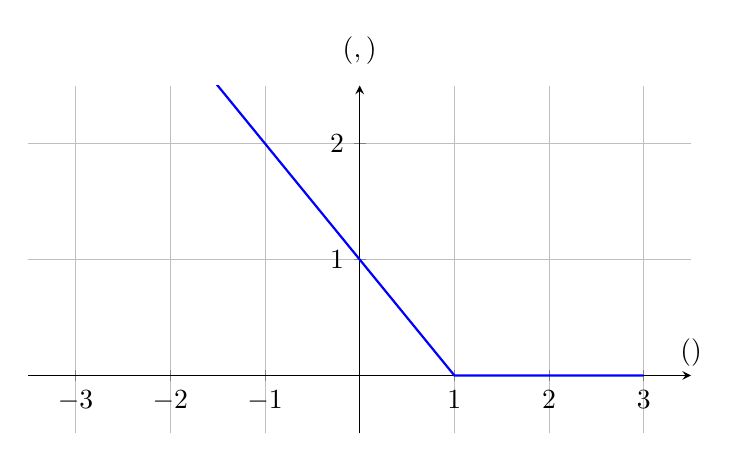
\begin{tikzpicture}
    \begin{axis}[
        axis lines=middle,
        xlabel={$\truelabel\hypothesis(\featurevec)$},
        ylabel={$\lossfunc{(\featurevec,\truelabel)}{\hypothesis}$},
 	xlabel style={at={(axis description cs:1.,0.3)}, anchor=north},  % Adjusted to be relative to axis end
        ylabel style={at={(axis description cs:0.5,1.1)}, anchor=center}, % Corrected to vertical position, rotated for readability
        xmin=-3.5, xmax=3.5,
        ymin=-0.5, ymax=2.5,
        xtick={-3, -2, -1, 0, 1, 2, 3},
        ytick={0, 1, 2},
        domain=-3:3,
        samples=100,
        width=10cm, height=6cm,
        grid=both,
        major grid style={line width=.2pt, draw=gray!50},
        minor grid style={line width=.1pt, draw=gray!20},
        legend pos=south west % Positions legend at the bottom left
    ]
        \addplot[blue, thick] {max(0, 1-x)};
     %   \addlegendentry{$\max(0, 1-x)$}
    \end{axis}
\end{tikzpicture}
	%	\end{figure} 
		\end{center}
	    A regularized variant of the hinge \gls{loss} is used by the \gls{svm} \cite{LampertNowKernel}. 	    
		},first={hinge loss},text={hinge loss}}

\newglossaryentry{iidasspt}{name={independent and identically distributed assumption (i.i.d.\ assumption)}, description={The \gls{iid} 
		assumption\index{independent and identically distributed assumption (i.i.d.\ assumption)} interprets \gls{datapoint}s of a \gls{dataset} as the 
		\gls{realization}s of \gls{iid} \gls{rv}s.},first={independent and identically distributed assumption (i.i.d.\ assumption)},text={i.i.d.\ assumption} }

\newglossaryentry{ai}{name={intelligence artificielle (IA)}, description={
		AI\index{intelligence artificielle (IA)} refers to systems that behave rationally in the sense of 
		maximizing a long-term \gls{reward}. The \gls{ml}-based approach to AI is to train a \gls{model} for  
		predicting optimal actions. These predictions are computed from observations about the state of the 
		environment. The choice of \gls{lossfunc} sets AI applications apart from more basic \gls{ml} applications. 
		AI systems rarely have access to a labeled \gls{trainset} that allows the average \gls{loss} to be measured for any possible choice of \gls{modelparams}. 
		Instead, AI systems use observed \gls{reward} signals to obtain a (point-wise) estimate for the 
		\gls{loss} incurred by the current choice of \gls{modelparams}.},first={intelligence artificielle (IA)},text={IA} }

\newglossaryentry{reward}{name={reward}, description={A reward refers to some\index{reward} observed 
		(or measured) quantity that allows us to estimate the \gls{loss} incurred by the \gls{prediction} 
		(or decision) of a \gls{hypothesis} $\hypothesis(\featurevec)$. For example, in an 
		\gls{ml} application to self-driving vehicles, $\hypothesis(\featurevec)$ could represent 
		the current steering direction of a vehicle. We could construct a reward from the 
		measurements of a collision sensor that indicate if the vehicle is moving towards 
		an obstacle. We define a low reward for the steering direction 
	$\hypothesis(\featurevec)$ if the vehicle moves dangerously towards an obstacle.},
	first={reward}, text={reward}} 

\newglossaryentry{hardclustering}{name={hard clustering}, description={Hard \gls{clustering}\index{hard clustering} 
		refers to the task of partitioning a given set of \gls{datapoint}s into (a few) non-overlapping \gls{cluster}s. 
		The most widely used hard \gls{clustering} method is \gls{kmeans}.},first={hard clustering},text={hard clustering} }
	
\newglossaryentry{softclustering}{name={soft clustering}, description={Soft \gls{clustering}\index{soft clustering} 
		refers to the task of partitioning a given set of \gls{datapoint}s into (a few) overlapping \gls{cluster}s. 
		Each \gls{datapoint} is assigned to several different \gls{cluster}s with varying degrees of belonging. Soft \gls{clustering} 
		methods determine the \gls{dob} (or soft \gls{cluster} assignment) for each \gls{datapoint} and each \gls{cluster}.
		A principled approach to soft \gls{clustering} is by interpreting \gls{datapoint}s as \gls{iid} \gls{realization}s 
		of a \gls{gmm}. We then obtain a natural choice for the \gls{dob} as the conditional 
		\gls{probability} of a \gls{datapoint} belonging to a specific mixture component.},first={soft clustering},text={soft clustering} }
	
\newglossaryentry{clustering}{name={partitionnement de données}, description={Clustering\index{partitionnement de données} methods decompose a given 
		set of \gls{datapoint}s into a few subsets, which are referred to as \gls{cluster}s. 
		Each \gls{cluster} consists of \gls{datapoint}s that are more similar to each 
		other than to \gls{datapoint}s outside the \gls{cluster}. Different clustering methods 
		use different measures for the similarity between \gls{datapoint}s and different 
		forms of \gls{cluster} representations. The clustering method \gls{kmeans} uses the 
		average \gls{feature} vector (cluster \gls{mean}) of a \gls{cluster} as its representative. 
		A popular \gls{softclustering} method based on \gls{gmm} represents 
		a \gls{cluster} by a \gls{mvndist}.},first={partitionnement de données},text={partitionnement de données} }
	
\newglossaryentry{cluster}{name={cluster}, description={A\index{cluster} cluster is a subset of 
		\gls{datapoint}s that are more similar to each other than to the \gls{datapoint}s outside the cluster. 
		The quantitative measure of similarity between \gls{datapoint}s is a design choice. If \gls{datapoint}s 
		are characterized by Euclidean \gls{featurevec}s $\featurevec \in \mathbb{R}^{\nrfeatures}$, 
		we can define the similarity between two \gls{datapoint}s via the Euclidean distance between 
		their \gls{featurevec}s. An example of such clusters is shown in Figure~\ref{fig:clusters}.\\
		\begin{figure}
			\centering
			\begin{tikzpicture}
				\pgfplotsset{compat=1.18}
				\begin{axis}[
					width=10cm,
					height=8cm,
					xlabel={$x_1$},
					ylabel={$x_2$},
					title={Clusters of Data Points},
					xmin=0, xmax=10,
					ymin=0, ymax=10,
					axis lines=left,
					legend style={at={(0.5,-0.25)}, anchor=north, legend columns=3}
					]
					% Cluster 1 
					\addplot[only marks, color=blue, mark=*, mark size=3pt] coordinates {
						(1,1) (2,1.2) (1.8,2) (2.2,1.5) (1.5,2.5)
					};
					% Cluster 2 
					\addplot[only marks, color=red, mark=square*, mark size=3pt] coordinates {
						(7,8) (8,7.5) (7.5,8.5) (8.2,7.8) (7.7,7)
					};
					% Cluster 3 
					\addplot[only marks, color=green!60!black, mark=triangle*, mark size=3pt] coordinates {
						(5,3) (5.5,3.2) (5.2,2.8) (4.8,3.5) (5.1,3.1)
					};
					\legend{Cluster 1, Cluster 2, Cluster 3}
				\end{axis}
			\end{tikzpicture} 
			\caption{Illustration of three clusters in a two-dimensional feature space. Each cluster groups data points that are more similar to 		each other than to those in other clusters, based on Euclidean distance.}
			\label{fig:clusters}
		\end{figure}
	},
	first={cluster},text={cluster} }

%\newglossaryentry{softclustering}{name={soft clustering}, description={Soft clustering methods determine, for each \gls{datapoint} within a dataset, 
%		a soft cluster assignment or the degree of belonging to a particular cluster.},first={soft clustering},text={soft clustering} }


\newglossaryentry{huberloss}{name={Huber loss}, description={The\index{Huber loss} 
		Huber \gls{loss} unifies the \gls{sqerrloss} and the \gls{abserr}.},first={Huber loss},text={Huber loss} }

\newglossaryentry{svm}{name={support vector machine (SVM)}, description={The\index{support vector machine (SVM)} 
		SVM is a binary \gls{classification} method that 
		learns a linear \gls{hypothesis} map. Thus, like \gls{linreg} and \gls{logreg}, 
		it is also an instance of \gls{erm} for the \gls{linmodel}. However, the 
		SVM uses a different \gls{lossfunc} from the one used in those methods. As illustrated in 
		Figure \ref{fig_svm_gls_dict}, it aims to maximally separate \gls{datapoint}s from 
		the two different classes in the \gls{featurespace} (i.e., \gls{maximum} margin principle). 
		Maximizing this separation is equivalent to minimizing a regularized 
		variant of the \gls{hingeloss} \eqref{equ_hinge_loss_gls_dict} \cite{LampertNowKernel,Cristianini_Shawe-Taylor_2000,BishopBook}.
		\begin{figure}[H]
			\begin{center}
				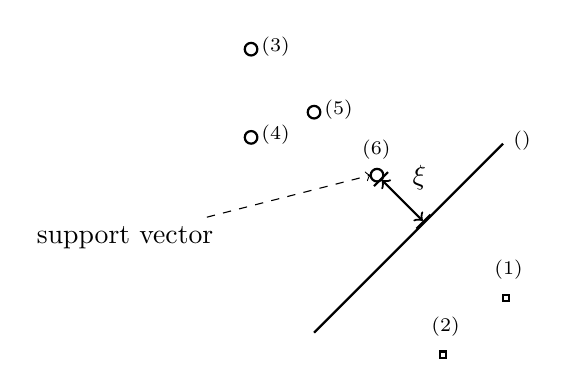
\begin{tikzpicture}[auto,scale=0.8]
					%\draw [thick] (0,-3) rectangle (4,4) node [anchor=east,above] {$\featurespace$} ;
					\draw [thick] (1,2) circle (0.1cm)node[anchor=west] {\hspace*{0mm}$\featurevec^{(5)}$};
					\draw [thick] (0,1.6) circle (0.1cm)node[anchor=west] {\hspace*{0mm}$\featurevec^{(4)}$};
					\draw [thick] (0,3) circle (0.1cm)node[anchor=west] {\hspace*{0mm}$\featurevec^{(3)}$};
					\draw [thick] (2,1) circle (0.1cm)node[anchor=east,above] {\hspace*{0mm}$\featurevec^{(6)}$};
					\node[] (B) at (-2,0) {support vector};
					\draw[->,dashed] (B) to (1.9,1) ; 
					\draw [|<->|,thick] (2.05,0.95)  -- (2.75,0.25)node[pos=0.5] {$\xi$} ; 
					\draw [thick] (1,-1.5) -- (4,1.5) node [right] {$\hypothesis^{(\weights)}$} ; 
					\draw [thick] (3,-1.9) rectangle ++(0.1cm,0.1cm) node[anchor=west,above]  {\hspace*{0mm}$\featurevec^{(2)}$};
					\draw [thick] (4,.-1) rectangle ++(0.1cm,0.1cm) node[anchor=west,above] {\hspace*{0mm}$\featurevec^{(1)}$};
				\end{tikzpicture}
				\caption{The \gls{svm} learns a \gls{hypothesis} (or \gls{classifier}) $\hypothesis^{(\weights)}$ with 
					minimal average soft-margin \gls{hingeloss}. Minimizing this \gls{loss} is equivalent 
					to maximizing the margin $\xi$ between the \gls{decisionboundary} of $\hypothesis^{(\weights)}$ 
					and each class of the \gls{trainset}.}
				\label{fig_svm_gls_dict}
			\end{center}
		\end{figure}
		The above basic variant of SVM is only useful if the \gls{datapoint}s from different categories can be  
		(approximately) linearly separated. For an \gls{ml} application where the categories are not 
		%linearly separable based on the the original (raw) \gls{feature}s it is possible to apply the SVM 
		%to transformed \gls{feature}s. These transformed \gls{feature}s can be obtained by applying a \gls{featuremap} 
		derived from a \gls{kernel}.
},first={support vector machine (SVM)},text={SVM} }
	
\newglossaryentry{eigenvector}{name={vecteur propre}, description={An\index{vecteur propre} 
		eigenvector of a matrix $\mathbf{A} \in \mathbb{R}^{\featuredim \times \featuredim}$ 
		is a non-zero vector $\vx \in \mathbb{R}^{\featuredim} \setminus \{ \mathbf{0} \}$ 
		such that $\mathbf{A} \vx = \lambda \vx$ with some \gls{eigenvalue} $\lambda$.},first={vecteur propre},text={vecteur propre} }

\newglossaryentry{evd}{name={décomposition en éléments propres}, 
	description={The\index{décomposition en éléments propres} \gls{eigenvalue} 
		decomposition for a square matrix $\mA \in \mathbb{R}^{\dimlocalmodel \times \dimlocalmodel}$ 
		is a factorization of the form 
		$$\mA = \mathbf{V} {\bm \Lambda} \mathbf{V}^{-1}.$$ 
		The columns of the matrix $\mV = \big( \vv^{(1)},\ldots,\vv^{(\dimlocalmodel)} \big)$ are the 
		\gls{eigenvector}s of the matrix $\mV$. The diagonal matrix 
		${\bm \Lambda} = {\rm diag} \big\{ \eigval{1},\ldots,\eigval{\dimlocalmodel} \big\}$ 
		contains the \gls{eigenvalue}s $\eigval{\featureidx}$ corresponding to the \gls{eigenvector}s $\vv^{(\featureidx)}$. 
		Note that the above decomposition exists only if the matrix $\mA$ is diagonalizable.},first={décomposition en éléments propres},text={décomposition en éléments propres} }

\newglossaryentry{svd}{name={décomposition en valeurs singulières}, 
  	description={The\index{décomposition en valeurs singulières} SVD  
  		for a matrix $\mA \in \mathbb{R}^{\samplesize \times \dimlocalmodel}$ 
		is a factorization of the form 
		$$\mA = \mathbf{V} {\bm \Lambda} \mathbf{U}^{T},$$ 
		with orthonormal matrices $\mV \in \mathbb{R}^{\samplesize \times \samplesize}$ 
		and $\mU \in \mathbb{R}^{\dimlocalmodel \times \dimlocalmodel}$ \cite{GolubVanLoanBook}. 
		The matrix ${\bm \Lambda} \in \mathbb{R}^{\samplesize \times \dimlocalmodel}$ is 
		only non-zero along the main diagonal, whose entries $\Lambda_{\featureidx,\featureidx}$ 
		are non-negative and referred to as singular values.
	},first={décomposition en valeurs singulières},text={décomposition en valeurs singulières} }


\newglossaryentry{tv}{name={total variation}, description={See \gls{gtv}\index{total variation}.},
	first={total variation},text={total variation} }

 \newglossaryentry{cvxclustering}{name={convex clustering}, 
 	description={Consider\index{convex clustering} a \gls{dataset} 
 	$\featurevec^{(1)},\ldots,\featurevec^{(\samplesize)} \in \mathbb{R}^{\nrfeatures}$. 
 	\Gls{convex} \gls{clustering} learns vectors $\weights^{(1)},\ldots,\weights^{(\samplesize)}$ by 
 	minimizing 
 	$$ \sum_{\sampleidx=1}^{\samplesize} \normgeneric{\featurevec^{(\sampleidx)} - \weights^{(\sampleidx)}}{2}^2 + 
 	\regparam \sum_{\nodeidx,\nodeidx' \in \nodes} \normgeneric{\weights^{(\nodeidx)} - \weights^{(\nodeidx')}}{p}.$$ 
	Here, $ \normgeneric{\vu}{p} \defeq \big( \sum_{\featureidx=1}^{\dimlocalmodel} |u_{\featureidx}|^{p} \big)^{1/p}$ 
	denotes the $p$-\gls{norm} (for $p\geq1$).  
	It turns out that many of the optimal vectors $\widehat{\weights}^{(1)},\ldots,\widehat{\weights}^{(\samplesize)}$ 
	coincide. A \gls{cluster} then consists of those \gls{datapoint}s $\sampleidx \in \{1,\ldots,\samplesize\}$ 
	with identical $\widehat{\weights}^{(\sampleidx)}$ \cite{JMLR:v22:18-694,Pelckmans2005}. 
 	  },
 		first={convex clustering},text={convex clustering} }

\newglossaryentry{sgd}{name={subgradient descent}, description={\Gls{subgradient}\index{subgradient descent} 
		descent is a \gls{generalization} of \gls{gd} that does not require differentiability of the 
		function to be minimized. This \gls{generalization} is obtained by replacing the concept 
		of a \gls{gradient} with that of a \gls{subgradient}. Similar to \gls{gradient}s, also \gls{subgradient}s 
		allow us to construct local approximations of an \gls{objfunc}. The \gls{objfunc} 
		might be the \gls{emprisk} $\emperror\big( \hypothesis^{(\weights)} \big| \dataset \big)$ viewed 
		as a function of the \gls{modelparams} $\weights$ that select a \gls{hypothesis} $\hypothesis^{(\weights)} \in \hypospace$.},first={subgradient descent},text={subgradient descent} }
	
\newglossaryentry{stochGD}{name={stochastic gradient descent (SGD)}, description={Stochastic\index{stochastic gradient descent (SGD)} 
		\gls{gd} is obtained from \gls{gd} by replacing the \gls{gradient} of the \gls{objfunc} 
		with a stochastic approximation. A main application of stochastic \gls{gd} 
		is to train a parametrized \gls{model} via \gls{erm} on a \gls{trainset} $\dataset$ that 
		is either very large or not readily available (e.g., when \gls{datapoint}s are stored 
		in a database distributed all over the planet). To evaluate the \gls{gradient} of the 
		\gls{emprisk} (as a function of the \gls{modelparams} $\weights$), 
		we need to compute a sum $\sum_{\sampleidx=1}^{\samplesize} \nabla_{\weights} \lossfunc{\datapoint^{(\sampleidx)}}{\weights}$  
		over all \gls{datapoint}s in the \gls{trainset}. We obtain a stochastic 
		approximation to the \gls{gradient} by replacing the sum $\sum_{\sampleidx=1}^{\samplesize} \nabla_{\weights} \lossfunc{\datapoint^{(\sampleidx)}}{\weights}$ 
		with a sum $\sum_{\sampleidx \in \batch} \nabla_{\weights} \lossfunc{\datapoint^{(\sampleidx)}}{\weights}$ 
		over a randomly chosen subset $\batch \subseteq \{1,\ldots,\samplesize\}$ (see Figure \ref{fig_sgd_approx_dict}). 
		We often refer to these randomly chosen \gls{datapoint}s as a \gls{batch}. 
		The \gls{batch} size $|\batch|$ is an important parameter of stochastic \gls{gd}. 
		Stochastic \gls{gd} with $|\batch|> 1$ is referred to as mini-\gls{batch} stochastic \gls{gd} \cite{Bottou99}. 		
		\begin{figure}[H]
			\centering
			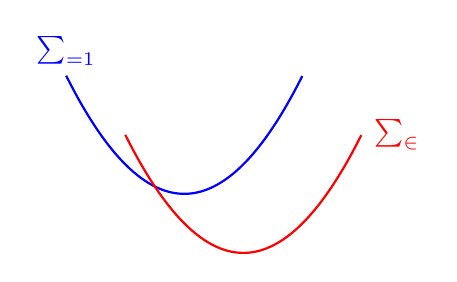
\begin{tikzpicture}[scale=1.5, >=stealth]
% Axes
				%\draw[->] (-1, 0) -- (4, 0) node[right] {$w$};
				%\draw[->] (0, -0.5) -- (0, 4) node[above] {};
% First quadratic function: f(w)
				\draw[thick, blue, domain=0.5:2.5, samples=100] plot (\x, {(\x-1.5)^2 + 1});
				\node[blue,above] at (0.5, 2) {$\sum_{\sampleidx=1}^{\samplesize}$};
% Second quadratic function: f'(w)
				\draw[thick, red, domain=1:3, samples=100] plot (\x, {(\x-2)^2 + 0.5});
				\node[red] at (3.3, 1.5) {$\sum_{\sampleidx \in \batch}$};
% Labels
			\end{tikzpicture}
		\caption{Stochastic \gls{gd} for \gls{erm} approximates the \gls{gradient} 
		$\sum_{\sampleidx=1}^{\samplesize} \nabla_{\weights} \lossfunc{\datapoint^{(\sampleidx)}}{\weights}$ 
		by replacing the 
		sum over all \gls{datapoint}s in the \gls{trainset} (indexed by $\sampleidx=1,\ldots,\samplesize$) 
		with a sum over a randomly chosen subset $\batch \subseteq \{1,\ldots,\samplesize\}$.\label{fig_sgd_approx_dict}}
		\end{figure}
},first={stochastic gradient descent (SGD)},text={SGD} }


\newglossaryentry{onlineGD}{name={online gradient descent (online GD)}, description={
Consider \index{online gradient descent (online GD)} an \gls{ml} method that learns \gls{modelparams} 
$\weights$ from some \gls{paramspace} $\paramspace \subseteq \mathbb{R}^{\dimlocalmodel}$. 
The learning process uses \gls{datapoint}s $\datapoint^{(\timeidx)}$ that arrive at consecutive time-instants $\timeidx=1,2,\ldots$. 
Let us interpret the \gls{datapoint}s $\datapoint^{(\timeidx)}$ as \gls{iid} copies 
of an \gls{rv} $\datapoint$. The \gls{risk} $\expect\{ \lossfunc{\datapoint}{\weights} \}$ of a 
\gls{hypothesis} $\hypothesis^{(\weights)}$ can then (under mild conditions) be obtained as the limit 
$\lim_{T\rightarrow \infty} (1/T)\sum_{\timeidx=1}^{T} \lossfunc{\datapoint^{(\timeidx)}}{\weights}$. 
We might use this limit as the \gls{objfunc} for learning the \gls{modelparams} $\weights$. 
Unfortunately, this limit can only be evaluated if we wait infinitely long in order to collect all \gls{datapoint}s. 
Some \gls{ml} applications require methods that learn online: as soon as a new \gls{datapoint} $\datapoint^{(\timeidx)}$ 
arrives at time $\timeidx$, we update the current \gls{modelparams} $\weights^{(\timeidx)}$. Note that 
the new \gls{datapoint} $\datapoint^{(\timeidx)}$ contributes the component $\lossfunc{\datapoint^{(\timeidx)}}{\weights}$ 
to the \gls{risk}. As its name suggests, online \gls{gd} updates $\weights^{(\timeidx)}$ via a (projected) \gls{gradstep}
\begin{equation} 
\label{equ_def_ogd_dict}
 \weights^{(\timeidx+1)} \defeq \projection{\paramspace}{\weights^{(\timeidx)} - \lrate_{\timeidx} \nabla_{\weights} \lossfunc{\datapoint^{(\timeidx)}}{\weights}}. 
\end{equation} 
Note that \eqref{equ_def_ogd_dict} is a \gls{gradstep} for the current component $\lossfunc{\datapoint^{(\timeidx)}}{\cdot}$ 
of the \gls{risk}. The update \eqref{equ_def_ogd_dict} ignores all the previous components $\lossfunc{\datapoint^{(\timeidx')}}{\cdot}$, 
for $\timeidx' < \timeidx$. It might therefore happen that, compared to $\weights^{(\timeidx)}$, the updated \gls{modelparams} 
$\weights^{(\timeidx+1)}$ increase the retrospective average \gls{loss} $\sum_{\timeidx'=1}^{\timeidx-1} \lossfunc{\datapoint^{(\timeidx')}}{\cdot}$. 
However, for a suitably chosen \gls{learnrate} $\lrate_{\timeidx}$, online \gls{gd} can be shown 
to be optimal in practically relevant settings. By optimal, we mean that the \gls{modelparams} 
$\weights^{(T+1)}$ delivered by online \gls{gd} after observing $T$ \gls{datapoint}s $\datapoint^{(1)},\ldots, \datapoint^{(T)}$ 
are at least as good as those delivered by any other learning method \cite{HazanOCO,GDOptimalRakhlin2012}. 
\begin{figure}[H]
	\begin{center}
\begin{tikzpicture}[x=1.5cm,scale=1.5, every node/.style={font=\footnotesize}]
	% Axes
	\draw[->] (0.5, 0) -- (5.5, 0) node[below] {};
	%\draw[->] (0, -0.5) -- (0, 3) node[left] {Value};
	% Labels for time steps
	\foreach \x in {1, 2, 3, 4, 5} {
		\draw (\x, 0.1) -- (\x, -0.1) node[below] {$t=\x$};
	}
	% Data points (black circles)
	\foreach \x/\y in {1/2.5, 2/1.8, 3/2.3, 4/1.5, 5/2.0} {
		\fill[black] (\x, \y) circle (2pt) node[above right] {$\datapoint^{(\x)}$};
	}
	% Model parameters (blue circles)
	\foreach \x/\y in {1/1.0, 2/1.6, 3/1.8, 4/2.2, 5/1.9} {
		\fill[blue] (\x, \y) circle (2pt) node[below left] {$\weights^{(\x)}$};
	}
	% Connecting lines (model tracking data)
	\foreach \x/\y/\z in {1/2.5/1.0, 2/1.8/1.6, 3/2.3/2.0, 4/1.5/1.8, 5/2.0/1.9} {
		\draw[dashed, gray] (\x, \y) -- (\x, \z);
	}
	% Legend
	% \node[draw, fill=white] at (4.5, 2.7) {
	% 	\begin{tabular}{@{}ll@{}}
	% 		\textcolor{black}{$\bullet$} & Data Point ($d_t$) \\
	% 		\textcolor{blue}{$\bullet$} & Model Parameter ($\theta_t$) \\
	% 		\textcolor{gray}{\rule{1cm}{0.5pt}} & Gradient Update
	% 	\end{tabular}
	%};
	\end{tikzpicture}
\end{center} 
\caption{An instance of online \gls{gd} that updates the \gls{modelparams} $\weights^{(\timeidx)}$ 
using the \gls{datapoint} $\datapoint^{(\timeidx)} = \feature^{(\timeidx)}$ arriving at time $\timeidx$. 
This instance uses the \gls{sqerrloss} $\lossfunc{\datapoint^{(\timeidx)}}{\weight} = (\feature^{(\timeidx)} - \weight)^{2}$.
}
\end{figure}},
first={online gradient descent (online GD)},text={online GD}}

\newglossaryentry{pca}{name={analyse en composantes principales (ACP)}, description={PCA\index{analyse en composantes principales (ACP)} 
		determines a linear \gls{featuremap} such that the new \gls{feature}s 
		allow us to reconstruct the original \gls{feature}s with the \gls{minimum} reconstruction error \cite{MLBasics}.},first={analyse en composantes principales (ACP)},text={ACP} }

\newglossaryentry{decisiontree}{name={arbre de décision}, description={A\index{arbre de décision} 
		decision tree is a flow-chart-like representation of a \gls{hypothesis} map $\hypothesis$. 
		More formally, a decision tree is a directed \gls{graph} containing a root node that reads 
		in the \gls{featurevec} $\featurevec$ of a \gls{datapoint}. The root node then forwards 
		the \gls{datapoint} to one of its children nodes based on some elementary test on the \gls{feature}s $\featurevec$. 
		If the receiving child node is not a leaf node, i.e., it has itself children nodes, 
	  it represents another test. Based on the test result, the \gls{datapoint} is forwarded 
	   to one of its descendants. This testing and forwarding of the \gls{datapoint} is continued 
	  until the \gls{datapoint} ends up in a leaf node (having no children nodes). 
\begin{figure}[H]
\begin{minipage}{.45\textwidth}
	\scalebox{1}{
\begin{tikzpicture}
%	% Root node
	\node[fill=black, circle, inner sep=2pt, label=above:{$\| \featurevec-\mathbf{u} \| \leq \varepsilon$?}] (A) {};	
%	% Left child (h1)
	\node[fill=black, circle, inner sep=2pt, below left=1.5cm and 1cm of A, label=left:{$\hypothesis(\featurevec) = \predictedlabel_1$}] (B) {};
	% Right child (next question)
	\node[fill=black, circle, inner sep=2pt, below right=1.5cm and 1cm of A, label=right:{$\| \featurevec - \mathbf{v} \| \leq \varepsilon$?}] (C) {};
%	% Left child of C (h2)
	\node[fill=black, circle, inner sep=2pt, below left=1.5cm and 1cm of C, label=left:{$\hypothesis(\featurevec) = \predictedlabel_2$}] (D) {};
	% Right child of C (h3)
	\node[fill=black, circle, inner sep=2pt, below right=1.5cm and 1cm of C, label=right:{$\hypothesis(\featurevec) =\predictedlabel_3$}] (E) {};
%	% Arrows
	\draw[line width=1.5pt, ->] (A) -- (B) node[midway, left] {no};
	\draw[line width=1.5pt, ->] (A) -- (C) node[midway, right] {yes};
	\draw[line width=1.5pt, ->] (C) -- (D) node[midway, left] {no};
	\draw[line width=1.5pt, ->] (C) -- (E) node[midway, right] {yes};
\end{tikzpicture}
	}
\end{minipage}	
\hspace*{15mm}
\begin{minipage}{.45\textwidth}
	\hspace*{15mm}
	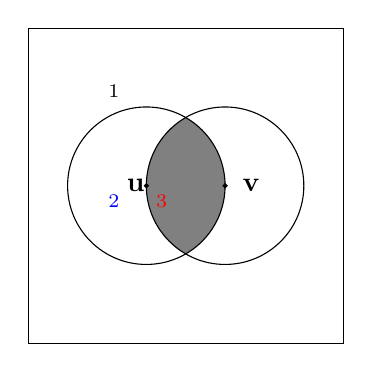
\begin{tikzpicture}
		\draw (-2,2) rectangle (2,-2);
		\begin{scope}
			\clip (-0.5,0) circle (1cm);
			\clip (0.5,0) circle (1cm);
			\fill[color=gray] (-2,1.5) rectangle (2,-1.5);
		\end{scope}
		\draw (-0.5,0) circle (1cm);
		\draw (0.5,0) circle (1cm);
		\draw[fill] (-0.5,0) circle [radius=0.025];
		\node [below right, red] at (-0.5,0) {$\predictedlabel_{3}$};
		\node [below left, blue] at (-0.7,0) {$\predictedlabel_{2}$};
		\node [above left] at (-0.7,1) {$\predictedlabel_{1}$};
		\node [left] at (-0.4,0) {$\mathbf{u}$};
		\draw[fill] (0.5,0) circle [radius=0.025];
		\node [right] at (0.6,0) {$\mathbf{v}$};
	\end{tikzpicture}
\end{minipage}
	\caption{Left: A decision tree is a flow-chart-like representation of a piece-wise constant \gls{hypothesis} $\hypothesis: \featurespace \rightarrow \mathbb{R}$.  Each piece is a \gls{decisionregion} $\decreg{\predictedlabel} \defeq \big\{ \featurevec \in  \featurespace: \hypothesis(\featurevec) = \predictedlabel \big\}$. 
		The depicted decision tree can be applied to numeric \gls{featurevec}s, i.e., $\featurespace \subseteq \mathbb{R}^{\dimlocalmodel}$. It is  parametrized by the threshold $\varepsilon>0$ and the vectors $\vu, \vv \in \mathbb{R}^{\dimlocalmodel}$. 
		Right: A decision tree partitions  
		the \gls{featurespace} $\featurespace$ into \gls{decisionregion}s. Each \gls{decisionregion}  
		$\decreg{\hat{\truelabel}} \!\subseteq\!\featurespace$ corresponds to a specific leaf node in the decision tree.}
	\label{fig_decision_tree}
\end{figure} 
	  }
	  ,first={arbre de décision},text={arbre de décision} }

%\newglossaryentry{API} 
%{
%	name={application programming interface (API)},
%	description={An\index{application programming interface} application programming 
%		interface (API) is a precise specification of the services and resources 
%		offered by software or hardware implementing that API.},
%	first={application programming interface (API)},
%	text={API}
%}


\newglossaryentry{API} 
{name={application programming interface (API)},
	description={
		An \index{application programming interface (API)} API is a formal mechanism that 
		allows software components to interact in a structured and modular way \cite{RestfulBook2013}.
		In the context of \gls{ml}, APIs are commonly used to provide access to a trained \gls{ml} \gls{model}. 
		Users—whether humans or machines—can submit the \gls{featurevec} of a \gls{datapoint} and receive 
		a corresponding \gls{prediction}. Suppose a trained \gls{ml} \gls{model} is defined 
		as $\widehat{\hypothesis}(\feature) \defeq 2 \feature + 1$. Through an API, a user 
		can input $\feature = 3$ and receive the output $\widehat{\hypothesis}(3) = 7$ 
		without knowledge of the detailed structure of the \gls{ml} \gls{model} or its training. 
		In practice, the \gls{model} is typically deployed on a server connected to the internet. 
		Clients send requests containing \gls{feature} values to the server, which responds with 
		the computed prediction $\widehat{\hypothesis}(\featurevec)$. APIs promote modularity 
		in \gls{ml} system design: one team can develop and train the model, while another 
		handles integration and user interaction. Publishing a trained \gls{model} via an API also 
		offers practical advantages: 
		\begin{itemize} 
			\item The server can centralize computational resources which are required to compute \gls{prediction}s. 
			\item The internal structure of the \gls{model} remains hidden (useful for protecting IP or trade secrets). 
		\end{itemize} 
		However, APIs are not without risk: techniques such as \gls{modelinversion} can potentially reconstruct a 
		\gls{model} from its \gls{prediction}s on carefully selected \gls{featurevec}s. 
	},
	first={application programming interface (API)},
	text={API}
}

\newglossaryentry{modelinversion}{name={model inversion},description={TBD.},first={model inversion},text={model inversion}}

\newglossaryentry{hilbertspace}{
	name={Hilbert space},
	description={A\index{Hilbert space} Hilbert space is a complete inner 
		product space \cite{introhilbertbook}. That is, it is a vector space equipped 
		with an inner product between pairs of vectors, and it satisfies the additional requirement 
		of completeness: every Cauchy sequence of vectors converges to a limit within the space. 
		A canonical example of a Hilbert space is the \gls{euclidspace} $\mathbb{R}^{\featuredim}$, 
		for some dimension $\featuredim$, consisting of vectors $\vu = \big(u_1, \ldots, u_{\featuredim}\big)^T$ 
		and the standard inner product $\vu^T \vv$.},
	first={Hilbert space},
	text={Hilbert space}
}


\newglossaryentry{sample}{name={sample},description={A\index{sample} 
		finite sequence (or list) of \gls{datapoint}s $\datapoint^{(1)},\ldots,\datapoint^{(m)}$ that 
		is obtained or interpreted as the \gls{realization} of $\samplesize$ \gls{iid} \gls{rv}s 
		with a common \gls{probdist} $p(\datapoint)$. The length $\samplesize$ of 
		the sequence is referred to as the \gls{samplesize}.},first={sample},text={sample}}

\newglossaryentry{randomforest}
{name={random forest},
	description={A\index{random forest} random forest is a set of different \gls{decisiontree}s. 
		Each of these \gls{decisiontree}s is obtained by fitting a perturbed copy of 
		the original \gls{dataset}.},first = {forêt d'arbres décisionnels}, text={forêt d'arbres décisionnels}
}

\newglossaryentry{bagging}{name={bagging},description={Bagging\index{bagging} (or bootstrap aggregation) 
		is a generic technique to improve (the robustness of) a given \gls{ml} method. The idea is to use the \gls{bootstrap} 
		to generate perturbed copies of a given \gls{dataset} and then to learn a separate \gls{hypothesis} for 
		each copy. We then predict the \gls{label} of a \gls{datapoint} by combining or aggregating the individual 
		\gls{prediction}s of each separate \gls{hypothesis}. For \gls{hypothesis} maps delivering numeric \gls{label} 
		values, this aggregation could be implemented by computing the average of individual \gls{prediction}s.},first={bootstrap aggregation (bagging)},text={bagging}}

\newglossaryentry{gd}{name={descente de gradient},description={\Gls{gradient}\index{descente de gradient} 
		descent is an iterative method for finding the \gls{minimum} of a \gls{differentiable} function $f(\weights)$ 
		of a vector-valued argument $\weights \in \mathbb{R}^{\featurelen}$. Consider a current guess or 
		approximation $\weights^{(\itercntr)}$ for the \gls{minimum} of the function $f(\weights)$. We would like to find a new (better) vector $\weights^{(\itercntr+1)}$ 
		that has a smaller objective value $f(\weights^{(\itercntr+1)}) < f\big(\weights^{(\itercntr)}\big)$ than 
		the current guess $\weights^{(\itercntr)}$. We can achieve this typically by using a \gls{gradstep}
		\begin{equation} 
			\label{equ_def_GD_step_dict}
			\weights^{(\itercntr\!+\!1)} = \weights^{(\itercntr)} - \lrate \nabla f(\weights^{(\itercntr)})
		\end{equation} 
		with a sufficiently small \gls{stepsize} $\lrate\!>\!0$. Figure \ref{fig_basic_GD_step_dict} illustrates the effect of 
		a single \gls{gradient} descent step \eqref{equ_def_GD_step_dict}.
		\begin{figure}[H]
			\begin{center}
				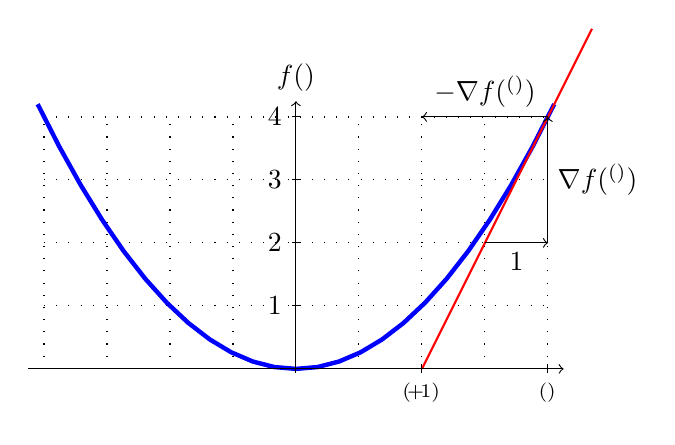
\begin{tikzpicture}[scale=0.8]
					\draw[loosely dotted] (-4,0) grid (4,4);
					\draw[blue, ultra thick, domain=-4.1:4.1] plot (\x,  {(1/4)*\x*\x});
					\draw[red, thick, domain=2:4.7] plot (\x,  {2*\x - 4});
					\draw[<-] (4,4) -- node[right] {$\nabla f(\weights^{(\itercntr)})$} (4,2);
					\draw[->] (4,4) -- node[above] {$-\lrate \nabla f(\weights^{(\itercntr)})$} (2,4);
					\draw[<-] (4,2) -- node[below] {$1$} (3,2) ;
					\draw[->] (-4.25,0) -- (4.25,0) node[right] {$\weights$};
					\draw[->] (0,-2pt) -- (0,4.25) node[above] {$f(\weights)$};
					\draw[shift={(0,0)}] (0pt,2pt) -- (0pt,-2pt) node[below] {$\overline{\weights}$};
					\draw[shift={(4,0)}] (0pt,2pt) -- (0pt,-2pt) node[below] {$\weights^{(\itercntr)}$};
					\draw[shift={(2,0)}] (0pt,2pt) -- (0pt,-2pt) node[below] {$\weights^{(\itercntr\!+\!1)}$};
					\foreach \y/\ytext in {1/1, 2/2, 3/3, 4/4}
					\draw[shift={(0,\y)}] (2pt,0pt) -- (-2pt,0pt) node[left] {$\ytext$};  
				\end{tikzpicture}
			\end{center}
			\caption{A single \gls{gradstep} \eqref{equ_def_GD_step_dict} towards the minimizer $\overline{\weights}$ of $f(\weights)$.}
			\label{fig_basic_GD_step_dict}
		\end{figure}
%		
		},first={descente de gradient},text={descente de gradient}}

\newglossaryentry{abserr}{name={absolute error loss},description={
			Consider a \gls{datapoint} with \gls{feature}s $\featurevec \in \featurespace$ and numeric 
			\gls{label} $\truelabel \in \mathbb{R}$. The absolute error \gls{loss}\index{absolute error loss} 
			incurred by a \gls{hypothesis} $\hypothesis: \featurespace \rightarrow \mathbb{R}$ 
			is defined as $|\truelabel - \hypothesis(\featurevec)|$, i.e., the absolute difference between 
			the \gls{prediction} $\hypothesis(\featurevec)$ and the true \gls{label} $\truelabel$.},
	%		{\bf Example.} Imagine you are predicting the temperature for tomorrow. If the actual 
	%		temperature is 20 (measured in degree Celsius), but your model predicts 18, the absolute 
	%		error is $20−18=2$. This means your prediction was off by $2$ (degrees Celius). 
	%		The absolute error loss always gives a positive number, so it doesn't matter if the \gls{prediction} 
	%		is too high or too low - only the size of the difference matters.}
			first={absolute error loss},text={absolute error loss}}

\newglossaryentry{llm}{name={grand modèle de langage (GML)},description={
	Large language \gls{model}s\index{grand modèle de langage (GML)} is an umbrella term for \gls{ml} methods 
	that process and generate human-like text. These methods typically 
	use \gls{deepnet}s with billions (or even trillions) of \gls{parameters}. 
	A widely used choice for the network architecture is referred to as 
	Transformers \cite{vaswani2017attention}. The training of large language \gls{model}s is often  
	based on the task of predicting a few words that are intentionally removed 
	from a large text corpus. Thus, we can construct \gls{labeled datapoint}s 
	simply by selecting some words of a text as \gls{label}s and the remaining 
	words as \gls{feature}s of \gls{datapoint}s. This construction requires 
	very little human supervision and allows for generating sufficiently 
	large \gls{trainset}s for large language \gls{model}s.},
					first={grand modèle de langage (GML)},text={GML}}


\newglossaryentry{huberreg}{name={Huber regression},description={
			Huber \gls{regression}\index{Huber regression} refers to \gls{erm}-based methods 
			that use the \gls{huberloss} as a measure of the \gls{prediction} error. 
			Two important special cases of Huber \gls{regression} are \gls{ladregression} and 
			\gls{linreg}. Tuning the threshold parameter of the \gls{huberloss} allows the user
			to trade the robustness of the \gls{abserr} 
			against the computational benefits of the \gls{smooth} \gls{sqerrloss}.},
			first={Huber regression},text={Huber regression}}


\newglossaryentry{ladregression}{name={least absolute deviation regression},description={
		Least\index{least absolute deviation regression} absolute deviation regression is 
		an instance of \gls{erm} using the \gls{abserr}. It is a special case of 
		\gls{huberreg}.},
		first={least absolute deviation regression},text={least absolute deviation regression}}

\newglossaryentry{bayesrisk}{name={Bayes risk},description={Consider a \gls{probmodel} with a 
joint \gls{probdist} $p(\featurevec,\truelabel)$ for the \gls{feature}s $\featurevec$ 
and \gls{label} $\truelabel$ of a \gls{datapoint}. The\index{Bayes risk} Bayes \gls{risk} 
is the \gls{minimum} possible \gls{risk} that can be achieved by any \gls{hypothesis} 
$\hypothesis: \featurespace \rightarrow \labelspace$. Any \gls{hypothesis} that achieves 
the Bayes risk is referred to as a \gls{bayesestimator} \cite{LC}.},first={Bayes risk},text={Bayes risk}}
	
\newglossaryentry{bayesestimator}{name={Bayes estimator},description={Consider\index{Bayes estimator} 
a \gls{probmodel} with a joint \gls{probdist} $p(\featurevec,\truelabel)$ for the \gls{feature}s $\featurevec$ and \gls{label} 
$\truelabel$ of a \gls{datapoint}. For a given \gls{lossfunc} $\lossfunc{\cdot}{\cdot}$, we refer to a \gls{hypothesis} 
$\hypothesis$ as a Bayes estimator if its \gls{risk} $\expect\{\lossfunc{\pair{\featurevec}{\truelabel}}{\hypothesis}\}$ is the 
\gls{minimum} \cite{LC}. Note that the property of a \gls{hypothesis} being a Bayes estimator depends on 
the underlying \gls{probdist} and the choice for the \gls{lossfunc} $\lossfunc{\cdot}{\cdot}$.},
		first={Bayes estimator},text={Bayes estimator}}

\newglossaryentry{lln}{name={law of large numbers},
	description={The\index{law of large numbers} law of large numbers refers to the 
		convergence of the average of an increasing (large) number of \gls{iid} \gls{rv}s 
		to the \gls{mean} of their common \gls{probdist}. Different instances of the 
		law of large numbers are obtained by using different notions of convergence \cite{papoulis}.},first={law of large numbers},text={law of large numbers}}
    
\newglossaryentry{stopcrit}{name={critère d'arrêt},
	description={Many\index{critère d'arrêt} \gls{ml} methods use iterative \gls{algorithm}s that construct a 
		sequence of \gls{modelparams} (such as the \gls{weights} of a linear map or 
		the \gls{weights} of an \gls{ann}). These parameters (hopefully) converge to an optimal choice 
		for the \gls{modelparams}. In practice, given finite computational 
		resources, we need to stop iterating after a finite number of repetitions. 
		A stopping criterion is any well-defined condition required for stopping 
		the iteration.},first={critère d'arrêt},text={critère d'arrêt}}

\newglossaryentry{kCV}{name={$k$-fold cross-validation ($\nrfolds$-fold CV)},
	description={$k$-fold CV\index{$k$-fold cross-validation ($\nrfolds$-fold CV)} is a 
		method for learning and validating a \gls{hypothesis} using a given \gls{dataset}. 
		This method divides the \gls{dataset} evenly into $k$ subsets or folds 
		and then executes $k$ repetitions of \gls{model} training (e.g., via \gls{erm}) and \gls{validation}. 
		Each repetition uses a different fold as the \gls{valset} and the remaining $k-1$ folds 
		as a \gls{trainset}. The final output is the average of the \gls{valerr}s obtained 
		from the $k$ repetitions.},first={$k$-fold cross-validation ($k$-fold CV)},text={$k$-fold CV}}
	
\newglossaryentry{renyidiv}{name={R\'enyi divergence}, 
	sort={Renyi},
	description={The R\'enyi divergence\index{R\'enyi divergence} measures the (dis)similarity 
		between two \gls{probdist}s \cite{RenyiInfo95}.}, 
	first = {R\'enyi divergence}, text = {R\'enyi divergence}} 

\newglossaryentry{nonsmooth}{name={non-smooth},
	description={We\index{non-smooth} refer to a function as non-smooth if it is not 
		\gls{smooth} \cite{nesterov04}.},first={non-smooth},text={non-smooth}}


\newglossaryentry{smooth}{name={lisse (ou régulière)},
	description={A\index{lisse (ou régulière)} real-valued function $f: \mathbb{R}^{\dimlocalmodel} \rightarrow \mathbb{R}$ 
		is smooth if it is \gls{differentiable} and its \gls{gradient} $\nabla f(\weights)$ is continuous at all $\weights \in \mathbb{R}^{\dimlocalmodel}$  \cite{nesterov04,CvxBubeck2015}. A smooth function $f$ is referred to as $\beta$-smooth if the \gls{gradient} 
		$\nabla f(\weights)$ is Lipschitz continuous with Lipschitz constant $\beta$, i.e., 
		$$\| \nabla f(\weights) - \nabla f(\weights') \| \leq \beta \| \weights - \weights' \| \mbox{, for any } \weights,\weights' \in \mathbb{R}^{\dimlocalmodel}.$$ 
		The constant $\beta$ quantifies the amount of smoothness of the function $f$: the smaller the $\beta$, 
		the smoother $f$ is. Optimization problems with a smooth \gls{objfunc} can be solved effectively by \gls{gdmethods}. 
	    Indeed, \gls{gdmethods} approximate the \gls{objfunc} locally around a current choice $\weights$ 
	    using its \gls{gradient}. This approximation works well if the \gls{gradient} does 
	    not change too rapidly. We can make this informal claim precise by studying the effect of a single 
	    \gls{gradstep} with \gls{stepsize} $\lrate=1/\beta$ (see Figure \ref{fig_gd_smooth_dict}). 
	    \begin{figure}[H] 
	    	\begin{center} 
	    	\begin{tikzpicture}[scale=0.8, x=0.7cm,y=0.05cm]
	    		% Parameter to shift the quadratic curve horizontally
	    		\def\hshift{0.5} % Change this value to shift the curve horizontally
	    		% Define the function (only the increasing part of x^2 for x >= 0)
	    		\draw[thick, domain=\hshift:8+\hshift, smooth, variable=\x] plot ({\x}, {\x^2}); %node[right] {$f(x) = x^2$};
	    		% Define points for the tangents
	    		\coordinate (w) at (\hshift,{\hshift*\hshift}); % Point w on the curve (left end of the plot)
	    		\coordinate (wkplus1) at (4+\hshift,{(4+\hshift)^2}); % Point w^{k+1} on the curve (x=1 + hshift, y=1)
	    		\coordinate (wk) at (8+\hshift,{(8+\hshift)^2}); % Point w^k on the curve (right end of the plot)
	    		% Calculate the slopes for the tangents
  				\draw[line width=1pt, transform canvas={yshift=-2pt}] (wk) -- +(-1, -{2*(8 + \hshift)} ) -- +(1, {2*(8 + \hshift)}); % Tangent at w^k with positive slope
 				\draw[line width=1pt, transform canvas={yshift=-2pt}] (w) -- +(-1, -{2*\hshift} ) -- +(1, {2*\hshift} )  node[below] {$\nabla f(\weights)$};% Tangent at w with slope 0 (since derivative at hshift = 0)
%	    		% Draw filled circles at points w^k, w, and w^{k+1}
	    		\filldraw (wk) circle (2pt) node[above left] {$\weights^{(\iteridx)}$} node[below right] {$\nabla f(\weights^{(\iteridx)})$} ;
	    		\filldraw (w) circle (2pt) node[above right] {$\weights$} ;
	    		\filldraw (wkplus1) circle (2pt) node[below right] {$\weights^{(\iteridx+1)}\!=\!\weights^{(\iteridx)}\!-\!(1/\beta)\nabla f(\weights^{(\iteridx)})$};
	    		    % Draw horizontal rulers to mark the function values at wk and wk_plus1
	    		\draw[dashed] (wk) -- ($(8,0) + (wk)$) ; %node[left] {$f(\weights^{(\iteridx)})$};
	    		\draw[dashed] (wkplus1) -- ($(12,0) + (wkplus1)$) ; %node[left] {$f(\weights^{(\iteridx+1)})$};
	    		 \draw[<->, thick] ($(4,0) + (wk)$) -- ($(8,0) + (wkplus1)$) 
	    		node[midway, right] {$ f\big(\weights^{(\iteridx)}\big)\!-\!f\big(\weights^{(\iteridx+1)}\big)\!\geq\!\frac{1}{2\beta}\normgeneric{\nabla f(\weights^{(\iteridx)})}{2}^{2}$};
%	    		% Label the curve
%	    		\node at (2, 4) {};
	    	\end{tikzpicture}
	    	\end{center}
	    	\caption{Consider an \gls{objfunc} $f(\weights)$ that is $\beta$-smooth. 
	    		Taking a \gls{gradstep}, with \gls{stepsize} $\lrate = 1/\beta$, decreases the 
	    		objective by at least $\frac{1}{2\beta}\normgeneric{\nabla f(\weights^{(\iteridx)})}{2}^{2}$ \cite{nesterov04,CvxAlgBertsekas,CvxBubeck2015}. 
	    		Note that the \gls{stepsize} $\lrate = 1/\beta$ becomes larger for smaller $\beta$. Thus, 
	    		for smoother \gls{objfunc}s (i.e., those with smaller $\beta$), 
				we can take larger steps. \label{fig_gd_smooth_dict}}
	    	\end{figure}
	    },first={lisse},text={lisse}}

\newglossaryentry{paramspace}{name={parameter space},
		description={The\index{parameter space} parameter space $\paramspace$ of 
		an \gls{ml} \gls{model} $\hypospace$ is the set of all feasible choices for the 
		\gls{modelparams} (see Figure \ref{fig_param_space_dict}). Many important \gls{ml} methods 
		use a \gls{model} that is parametrized by vectors of the \gls{euclidspace} $\mathbb{R}^{\dimlocalmodel}$. 
		Two widely used examples of parametrized \gls{model}s are \gls{linmodel}s 
		and \gls{deepnet}s. The parameter space is then often a subset $\paramspace \subseteq \mathbb{R}^{\dimlocalmodel}$, 
		e.g., all vectors $\weights \in \mathbb{R}^{\dimlocalmodel}$ with a \gls{norm} smaller than one.
		\begin{figure}[H]
			\begin{center}
			\begin{tikzpicture}
				% Left part: Ellipse representing parameter space (with two dots)
				\node[ellipse, minimum width=3cm, minimum height=2cm, draw, thick] (paramspace) {};
				\node[below=0.1cm of paramspace] {parameter space $\paramspace$};
				% Two dots inside the left ellipse
				\node[black, circle, inner sep=2pt, fill] (theta1) at ($(paramspace.north west) + (1, -1)$) {};
				\node[left=0.01cm of theta1] {$\weights$};
				\node[black, circle, inner sep=2pt, fill] (theta2) at ($(paramspace.south east) + (-1.5, 1)$) {};
				\node[left=0.01cm of theta2] {$\weights'$};
				% Right part: Ellipse containing two smaller plots
				\node[ellipse, minimum width=7cm, minimum height=3cm, draw, thick, right=4cm of paramspace] (plotcloud) {};
				\node[above=0.2cm of plotcloud] {\gls{model} $\hypospace$};
				% Axis for first smaller plot
				\node (plot1start) at ($(plotcloud.south west) + (0.2, 0.2)$) {};
				%\draw[thick, ->] (plot1start) -- ++(2, 0) node[anchor=north] {$\featurevec$};
				%\draw[thick, ->] (plot1start) -- ++(0, 1.5) node[anchor=east] {$\truelabel$};
				% Simple plot line in first smaller plot
				\draw[thick, red] (plot1start) .. controls ++(0.8, 1) and ++(-0.8, -0.8) .. ($(plotcloud.south west) + (2.8, 0.8)$) node[anchor=west] {$\hypothesis^{(\weights)}$};
				% Axis for second smaller plot
				\node (plot2start) at ($(plotcloud.south west) + (1.0, 1.2)$) {};
			%	\draw[thick, ->] (plot2start) -- ++(2, 0) node[anchor=north] {$\featurevec$};
			%	\draw[thick, ->] (plot2start) -- ++(0, 1.5) node[anchor=east] {$\truelabel$};
				% Simple plot line in second smaller plot
				\draw[thick, blue] (plot2start) .. controls ++(0.8, 0.5) and ++(-0.8, -0.8) .. ($(plotcloud.south west) + (2.8, 2.1)$) node[anchor=west] {$\hypothesis^{(\weights')}$};
				% Connect the two dots in the parameter space to the two plots
				\draw[thick, ->, bend right=20] (theta1) to ($(plot1start) + (0,0)$);
				\draw[thick, ->, bend left=20] (theta2) to (plot2start);
			\end{tikzpicture}
			\end{center} 
			\caption{The parameter space $\paramspace$ of an \gls{ml} \gls{model} $\hypospace$ consists of all 
			feasible choices for the \gls{modelparams}. Each choice $\weights$ for the \gls{modelparams} 
			selects a \gls{hypothesis} map $\hypothesis^{(\weights)} \in \hypospace$.
				 \label{fig_param_space_dict}} 
\end{figure}},
			first={parameter space},text={parameter space}}

\newglossaryentry{datanorm}{name={data normalization},
	description={\Gls{data} normalization\index{data normalization} refers to transformations 
		applied to the \gls{featurevec}s of \gls{datapoint}s to improve the \gls{ml} method's 
		\gls{statasp} or \gls{compasp}. For example, in \gls{linreg} with \gls{gdmethods} using 
		a fixed \gls{learnrate}, convergence depends on controlling the \gls{norm} of \gls{featurevec}s 
		in the \gls{trainset}. A common approach is to normalize \gls{featurevec}s such that their 
		\gls{norm} does not exceed one \cite[Ch.\ 5]{MLBasics}.},
	first={data normalization},text={data normalization}}

\newglossaryentry{dataaug}{name={data augmentation},
	description={\Gls{data} augmentation\index{data augmentation} methods add synthetic \gls{datapoint}s 
		to an existing set of \gls{datapoint}s. These synthetic \gls{datapoint}s are obtained by 
		perturbations (e.g., adding noise to physical measurements) or transformations 
		(e.g., rotations of images) of the original \gls{datapoint}s. These perturbations and 
		transformations are such that the resulting synthetic \gls{datapoint}s should 
		still have the same \gls{label}. As a case in point, a rotated cat image is still 
		a cat image even if their \gls{featurevec}s (obtained by stacking pixel color intensities) 
		are very different (see Figure \ref{fig_symmetry_dataaug_dict}). \Gls{data} augmentation can be an 
		efficient form of \gls{regularization}.
		\begin{figure}[H]
		\begin{center}
			\begin{tikzpicture}
				% Define shift macros locally
				\newcommand{\xshift}{0.5}
				\newcommand{\yshift}{2}
				% Define the shifted curves
				% Define the shifted curves
  				\draw[very thick, blue] plot[smooth, tension=1] coordinates {(0,0) (2,1) (4,0) (6,-1) (8,0)};
  				\node[blue, right] at (0,0) {\textbf{cat}};
  				\draw[very thick, red, dashed] plot[smooth, tension=1] coordinates {(0 + \xshift,0 + \yshift) (2 + \xshift,1 + \yshift) (4 + \xshift,0 + \yshift) (6 + \xshift,-1 + \yshift) (8 + \xshift,0 + \yshift)};
  				\node[red, right] at (8 + \xshift,0 + \yshift) {\textbf{no cat}};
				\fill[blue] (2,1) circle (2pt) node[above] {$\featurevec^{(1)}$};
				\fill[blue] (6,-1) circle (2pt) node[above] {$\featurevec^{(2)}$};
				  % Draw a bent arrow connecting the two points with custom in and out angles
				  \draw[->, thin, >=latex, line width=0.5pt] (2,1) to[out=240, in=240] node[midway, below] {$\mathcal{T}^{(\eta)}$} (6,-1);
			  \end{tikzpicture}
			  \vspace*{-11mm}
		\end{center}
		\caption{\Gls{data} augmentation exploits intrinsic symmetries of \gls{datapoint}s in 
		       some \gls{featurespace} $\featurespace$. We can represent a symmetry by 
		     an operator $\mathcal{T}^{(\eta)}: \featurespace \rightarrow \featurespace$,
		     parametrized by some number $\eta \in \mathbb{R}$. For example, $\mathcal{T}^{(\eta)}$ 
		    might represent the effect of rotating a cat image by $\eta$ degrees. A \gls{datapoint} 
		    with \gls{featurevec} $\featurevec^{(2)} = \mathcal{T}^{(\eta)} \big(\featurevec^{(1)} \big)$ must 
		    have the same \gls{label} $\truelabel^{(2)}=\truelabel^{(1)}$ as a \gls{datapoint} 
		     with \gls{featurevec} $\featurevec^{(1)}$.\label{fig_symmetry_dataaug_dict}}
		 \end{figure} },first={data augmentation},text={data augmentation}}
	
\newglossaryentry{localmodel}{name={local model},description={Consider\index{local model} a collection 
		of \gls{localdataset}s that are assigned to the nodes of an \gls{empgraph}. A local \gls{model} $\localmodel{\nodeidx}$ 
		is a \gls{hypospace} assigned to a node $\nodeidx \in \nodes$. Different nodes might be assigned 
		different \gls{hypospace}s, i.e., in general $\localmodel{\nodeidx} \neq \localmodel{\nodeidx'}$ for different 
		nodes $\nodeidx, \nodeidx' \in \nodes$.  },first={local model},text={local model}}
	
\newglossaryentry{mutualinformation}
{name={mutual information (MI)},
 description={The\index{mutual information (MI)} MI $\mutualinformation{\featurevec}{\truelabel}$ 
 	between two \gls{rv}s $\featurevec$, $\truelabel$ defined on the same \gls{probspace} 
 	is given by \cite{coverthomas} $$\mutualinformation{\featurevec}{\truelabel} \defeq 
	\expect \left\{ \log \frac{p (\featurevec,\truelabel)}{p(\featurevec)p(\truelabel)} \right\}.$$ 
	It is a measure of how well we can estimate $\truelabel$ based 
	solely on $\featurevec$. A large value of $\mutualinformation{\featurevec}{\truelabel}$ indicates that 
	$\truelabel$ can be well predicted solely from $\featurevec$. This \gls{prediction} could be obtained by a 
		\gls{hypothesis} learned by an \gls{erm}-based \gls{ml} method. 
	 }, first={MI}, text={MI} 
}

\newglossaryentry{zerogradientcondition}{name={zero-gradient condition},
	description={Consider\index{zero-gradient condition} the unconstrained 
		optimization problem $\min_{\weights \in \mathbb{R}^{\dimlocalmodel}} f(\weights)$  with 
			a \gls{smooth} and \gls{convex} \gls{objfunc} $f(\weights)$. A necessary and 
			sufficient condition for a vector $\widehat{\weights} \in \mathbb{R}^{\dimlocalmodel}$ 
			to solve this problem is that the \gls{gradient} $\nabla f \big( \widehat{\weights} \big)$ 
			is the zero vector, 
			$$ \nabla f \big( \widehat{\weights} \big) = \mathbf{0} \Leftrightarrow  f \big( \widehat{\weights} \big) = \min_{\weights \in \mathbb{R}^{\dimlocalmodel}} f(\weights) .$$ }, 
			first={zero-gradient condition},text={zero-gradient condition}}


\newglossaryentry{edgeweight}{name={edge weight},
	description={Each\index{edge weight} edge $\edge{\nodeidx}{\nodeidx'}$ of an \gls{empgraph} is 
		assigned a non-negative edge weight $\edgeweight_{\nodeidx,\nodeidx'}\geq0$. 
		A zero edge weight $\edgeweight_{\nodeidx,\nodeidx'}=0$ indicates the absence 
		of an edge between nodes $\nodeidx, \nodeidx' \in \nodes$.}, 
	first={edge weight},text={edge weight}}


\newglossaryentry{dataminprinc}{name={data minimization principle},
	description={European\index{data minimization principle} \gls{data} protection regulation 
		includes a \gls{data} minimization principle. This principle requires a \gls{data} controller to 
		limit the collection of personal information to what is directly relevant and necessary 
		to accomplish a specified purpose. The \gls{data} should be retained only for as long as 
		necessary to fulfill that purpose \cite[Article 5(1)(c)]{GDPR2016}, \cite{EURegulation2018}.}, 
	first={data minimization principle},text={data minimization principle}}


